% Author :  Lionel du Peloux
% Contact : lionel.dupeloux@gmail
% Year : 2017

\newrefsegment
\chapter{Elastic gridshells}\label{chp=gridshell}

\section{Introduction}
%===================

This chapter is meant to define and introduce what elastic gridshell structures are. It develops a comprehensive but precise view of the numerous knowledge and know-how that gravitate around this concept.

\subsection{Overview}
We naturally begin this chapter by defining the notion of elastic gridshell and the context in which this technology arose (see \cref{sec=gsdef}). We briefly highlight the benefits of composite materials for this kind of structure. We then propose two thorough reviews~: the first one is dedicated to known built elastic gridshell structures (see \cref{sec=review_project}) while the second one is a literature review of the main works related  to the topic of elastic gridshells (see \cref{sec=review_research}).

\subsection{Contributions}
%Here, we summarize our contributions that are presented in this chapter~:
\begin{itemize}
\item We establish a chronological review of known built elastic gridshells, from the very beginning of this technology to the present time. We reveal the richness of this concept by exhibiting the great variety of realised projects. We discuss the specificities brought by each one of these projects.
\item We establish an up-to-date review of the existing scientific literature, crossing multiple fields of research (geometry, mechanics, material, \telp{}).
\end{itemize}

\section{Definition}\label{sec=gsdef}

The invention of the \emph{elastic gridshell} concept is commonly attributed to Frei Otto, a German architect who devoted several years to gridshells. In 1975 he achieved the famous \emph{Mannheim Multihalle} \cite{Happold1975}, a wooden shell of 7500~m\textsuperscript{2}, in collaboration with the engineer Edmund Happold (Arup).
Literally, the word \textquote{gridshell} refers to grids behaving like shells~: from a mechanical point of view that means stresses acting on the structure are mainly transmitted through compression and tension. These structures can cross large-span with very little material.

However, according to the historic evolution of the concept, to characterise a gridshell as the combination of a structural concept (a grid behaving like a shell, see \cref{sec=def_topo}) and a specific construction process (see \cref{sec=def_erec}) using the bending flexibility of the material (see \cref{sec=def_flexibility}) seems to be more accurate. The project of Mannheim -- in which a wooden regular and planar grid, lacking shear stiffness, is elastically deformed up to a targeted shape with the help of stays, and then braced and covered -- is regarded as the starting point of this new concept (see \cref{fig:multihalle}).

The project of Mannheim is regarded as the starting point of this new concept for which a wooden regular and planar grid, lacking shear stiffness, is elastically deformed up to a targeted shape with the help of stays, and then braced and covered. This type of gridshell, known as elastic gridshell, offers a very elegant manner to materialise freeform shapes from an initially flat and regular grid, which obviously has many practical benefits~: planar initial geometry, standard connection nodes, standard profiles and so on.

Note that the term \emph{rigid gridshell} is often opposed to the term \emph{elastic gridshell} to indicate reticulated structures that behave like shells but are not formed in an active-bending process.

\subsection{Structural typology}\label{sec=def_topo}
% ------------------------------------------
Their mechanical behaviour is very similar to the one of real shells even if the material is discrete and located in a grid more or less open. Moreover, gridshells benefit from the same advantages as the ones showed by an eggshell : they can cross large span using a low amount of material. Their stiffness is mainly linked to their double-curved shape.


\subsection{Material flexibility for structural rigidity}\label{sec=def_flexibility}
% ------------------------------------------
In this field of application, composite materials like glass fibre reinforced polymer (GFRP) could favourably replace wood, where both resistance and bending ability of the material is sought \cite{Douthe2010a}. The stiffness of the structure does not derive from the intrinsic material rigidity but principally from its geometric curvature. Ideally, the composite profiles are produced by pultrusion, an economic continuous moulded process. The standardisation of the process guaranties very stable material and mechanical properties. It frees designers from the painful problematic of wood joining and wood durability. The characterisation of this material is presented further in the thesis (see \cref{sec=design_gfrp}).

\subsection{Erection process}\label{sec=def_erec}
% ------------------------------------------
Usually, the grid morphology is not trivial and leads to design numerous costly and complex joints. To overcome this issue, an original and innovative erection process was developed that takes advantage of the flexibility inherent to slender elements. A regular planar grid made of long continuous linear members is built on the ground (see \cref{fig:erec_1}). The elements are pinned together so the grid has no in-plane shear stiffness and can accommodate large-scale deformations during erection. Then, the grid is bent elastically to its final shape (see \cref{fig:erec_2}). Finally, the grid is frozen in the desired shape with a third layer of bracing members and the structure becomes a shell. This process is illustrated and detailed in the next chapter (see \cref{sec=construction_process}).

\begin{figure}[t]
		\subfloat[][Almost flat grid]{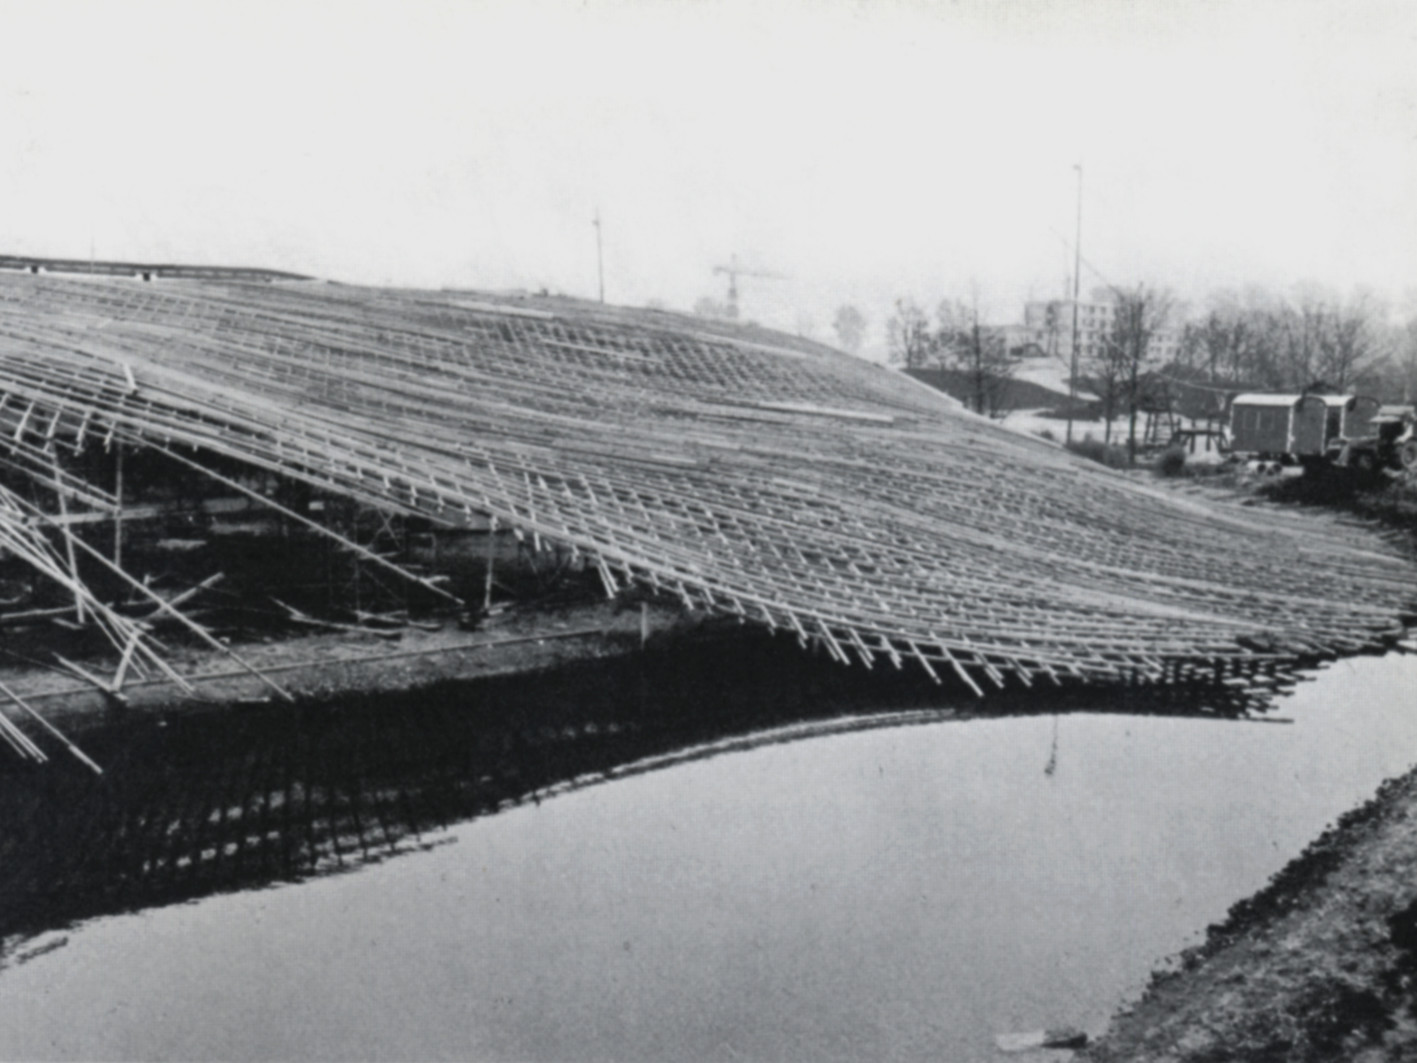
\includegraphics[width=0.48\textwidth]{mannheim_erection_1.jpg}\label{fig:erec_1}}
		\hspace*{\fill}
		\subfloat[][Deformed grid]{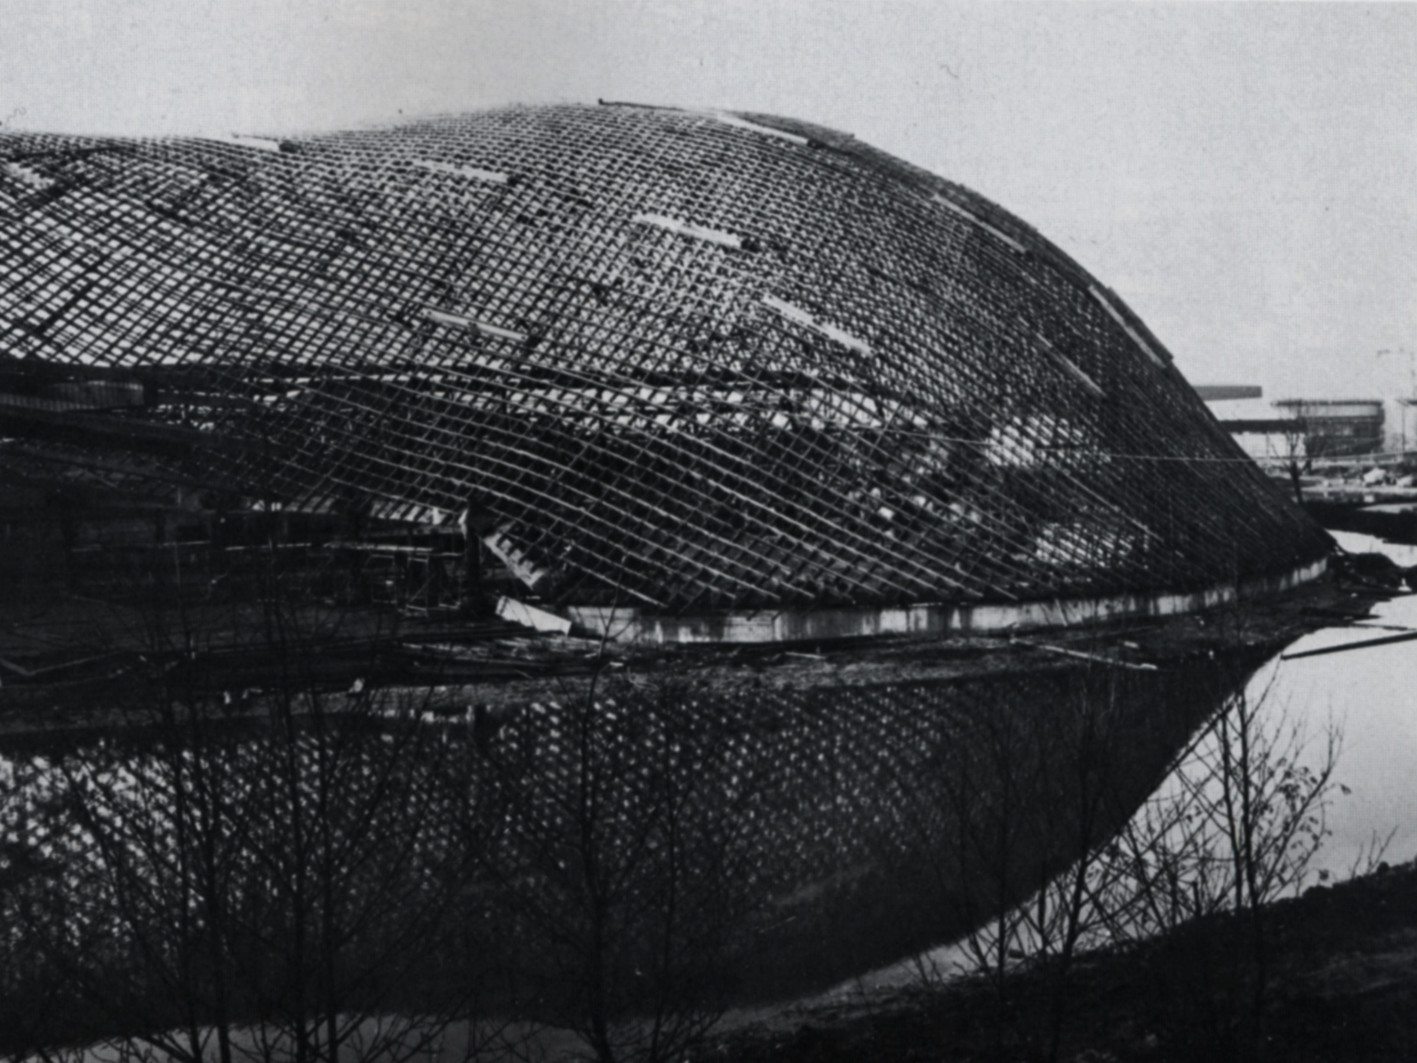
\includegraphics[width=0.48\textwidth]{mannheim_erection_2.jpg}\label{fig:erec_2}}
		%
		\vspace{10pt}
		\captionof{figure}[Forming process of the timber lattice of Mannheim, Germany]{Forming process of the timber lattice of Mannheim, Germany.}
		\label{fig:multihalle}
\end{figure}

\clearpage

\section{Built elastic gridshells : a review}\label{sec=review_project}

No thorough historic review is available about executed projects of elastic gridshells although some partial reviews have been done time to time on the occasion of scientific works or construction projects. This review aims at filling this gap by giving an overview of the development of the concept from the very beginning to the very last experiments. Only known built projects have been identified and reported here. The only condition for a project to belong to this review is to comply with the definition of what an elastic gridshell is (see \cref{sec=gsdef}), independently to any other consideration (material, fabrication, size, cladding,~\telp{}).

The informations collected during this research work are given in table format in appendix (see \cref{app:review}). A synthetic presentation of these datas is proposed to the reader in \cref{fig:projectsbymaterial}, where projects are ordered by date, span, covered area and material.

The books edited by the \emph{Institut für leichte Flächentragwerke} are of great interest to understand the beginnings. \citetitle{IL10} \cite{IL10} has a precise inventory of the first experiments from 1962 to 1976, while \citetitle{IL13} \cite{IL13} focuses on the construction of the Multihalle in Mannheim. \citetitle{Chilton2017} \cite{Chilton2017} is a significant effort but focuses exclusively on medium to large scale projects in timber. A small but general partial review is also available in \cite{Collins2016}. An interesting review is also given by \citet{Quinn2014} as part of their research work on new erection methods. A review of bracing and cladding systems is done in \cite{Cuvilliers2017}. A review of form-finding methods is done in \cite{Vaulot2016}. Finally, various valuable reviews are available in the thesis of \citet{Douthe2007,Bouhaya2010,Tayeb2015a,Lafuente2015}.
\begin{figure}[p]
\begin{fullpage}
	\centering
	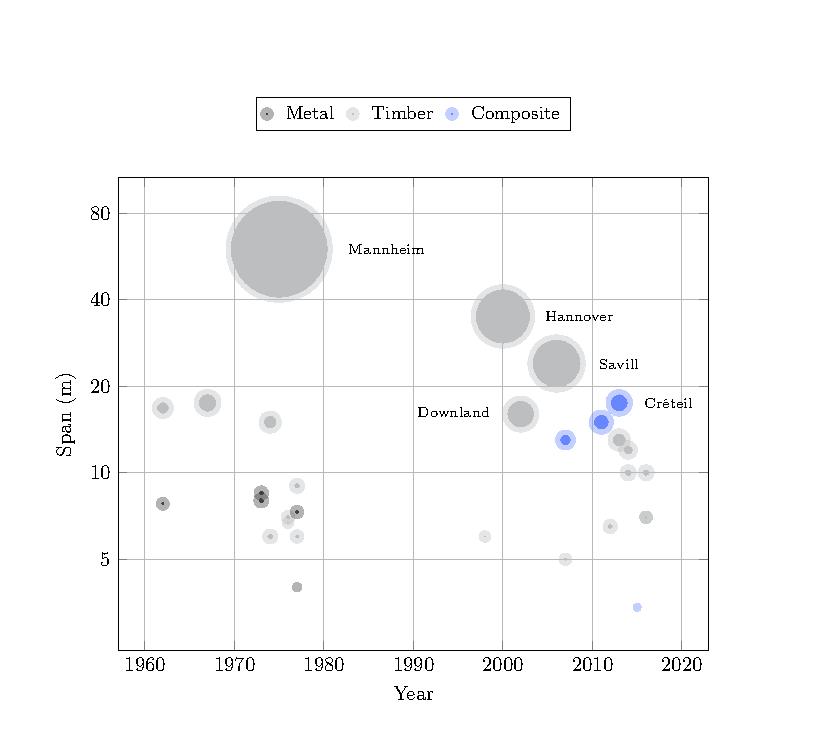
\includegraphics[]{ch2_gridshell/plot/1_projects/build.pdf}
	\caption[Known elastic gridshells built by the past.]{Known elastic gridshells built by the past. The surface of the bubbles is proportional to the covered area. Colour indicates the material employed for the rods.}
	\label{fig:projectsbymaterial}
\end{fullpage}
\end{figure}

\subsection{The beginnings : from the first prototype to the German Pavilion}
Frei Otto started his studies in architecture in 1947 in Berlin, Germany, and completed his doctorate on tensile structures in 1953. This first work was published and translated later in the 60's. He then began to work in the field of lightweight structures using physical models such as soap films or hanging nets, and photographic measurements.\footnote{In the 19\textsuperscript{th} and 20\textsuperscript{th} centuries model testing was at the heart of structural innovation \cite{Addis2013}. Analog models were employed successfully by well-known architects and engineers to go beyond the limits of existing knowledge (A. Gaudi, H. Isler, F. Candela, F. Otto, \telp{}) and are still employed today where numeric models failed to represent accurately some physical phenomenons (for instance in wind analysis for high rise towers and bridges).}\textsuperscript{,}\footnote{\blockcquote[p.~56]{IL10}{Photography is the medium through which the form and content of a model are communicated. It is one of our most important tools in that it provides the basis for documentation and information, supplements our creative potential \belp{} }} These tools were essentials for his exploration of forms and structures as there were no computers at that time.

\subsubsection{Steel Gridshell, Berkeley, USA, 1962}
Simultaneously, he became interested by the study of lightweight shells and the way they were form-found. One of his very first elastic gridshell was built in 1962 with students at Berkeley, USA \cite[p.~270]{IL10}. It is funny to remark that this first gridshell was not a timber gridshell but a steel gridshell made out of twin steel rods linked in a grid fashion by bolts with clamping plates (see \cref{fig:berkeley_a}). This first experiment demonstrated at small scale the ability to bend a regular grid with no shear rigidity into a curved shape  (see \cref{fig:berkeley_b}). The grid was loosely braced and shell effects were not investigated.

\subsubsection{Essen Gridshell, Essen, Germany, 1962}
The same year he designed and built a first timber gridshell in Essen, Germany \cite[p.~272]{IL10}. The prototype~-- a single-layer gridshell spanning \SI{17}{m} and covering an area of \SI{198}{m^2} -- was made with 3-plies laminated timber profiles in hemlock pine (see \cref{fig:essen_a}). The cross-section of the profiles was rectangular (\SI{60}{mm} x \SI{40}{mm}) and the elements were assembled in a grid fashion with simple steel bolts. Once erected, nothing was specifically done to improve the in-plane shear stiffness of the grid and activate a shell behaviour. Finally, the structure was covered with a transparent plastic foil nailed directly on the grid's profiles (see \cref{fig:essen_b}).

\begin{figure}[p]
     	\centering
	\begin{fullpage}
		\subfloat[][Knot detail]{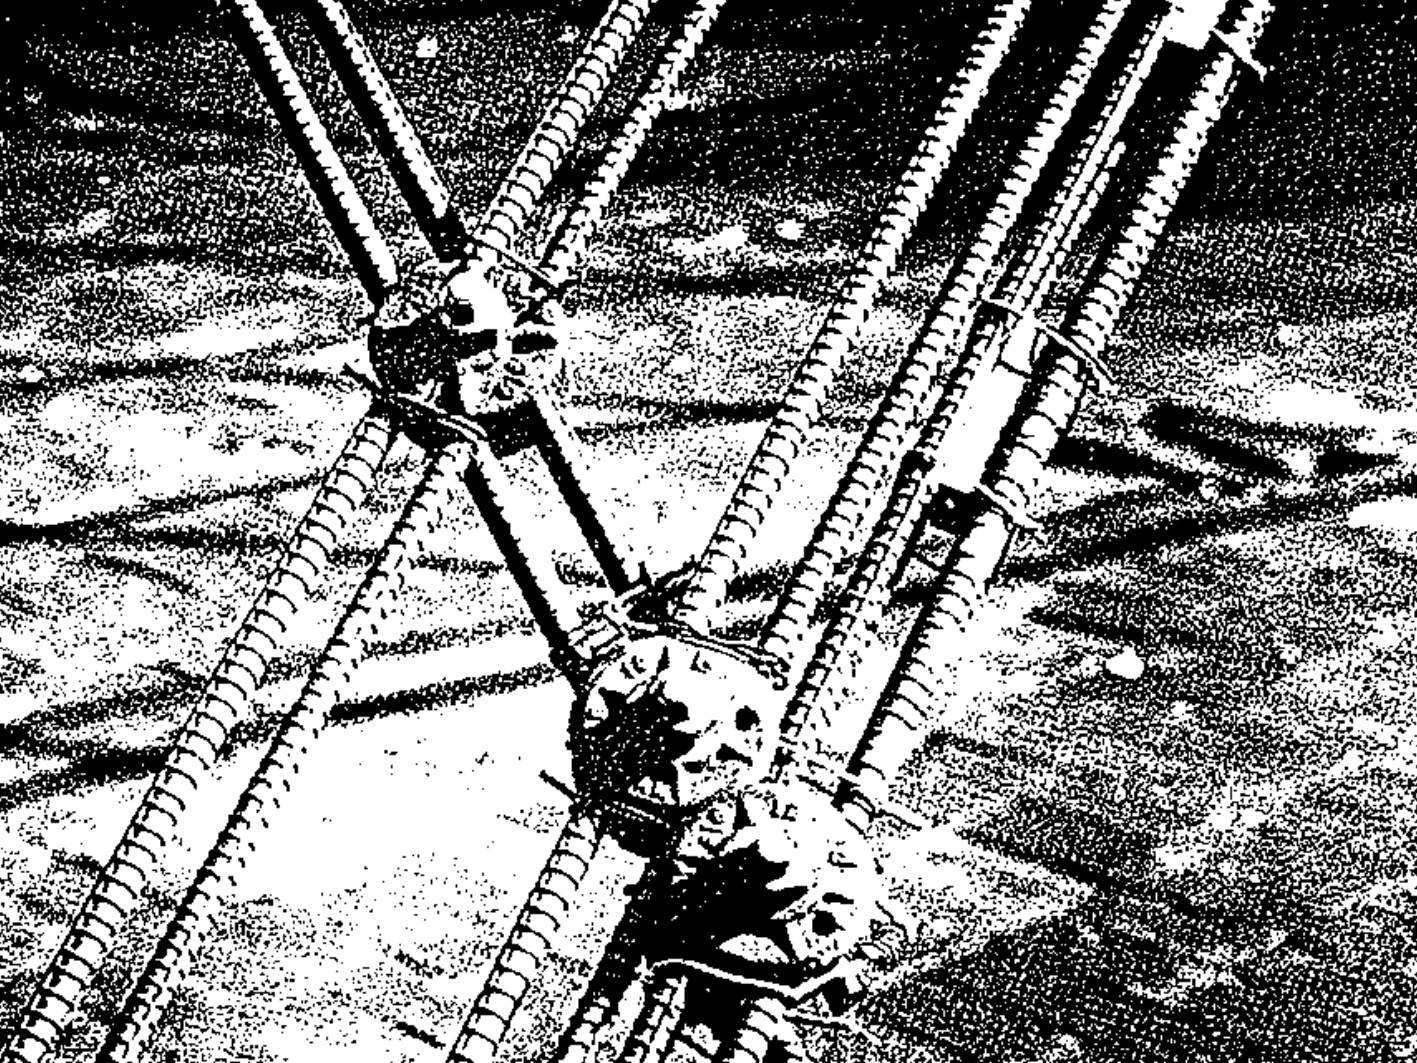
\includegraphics[width=0.48\textwidth]{berkeley_detail.jpg}\label{fig:berkeley_a}}
		\hspace*{\fill}
		\subfloat[][Steel lattice]{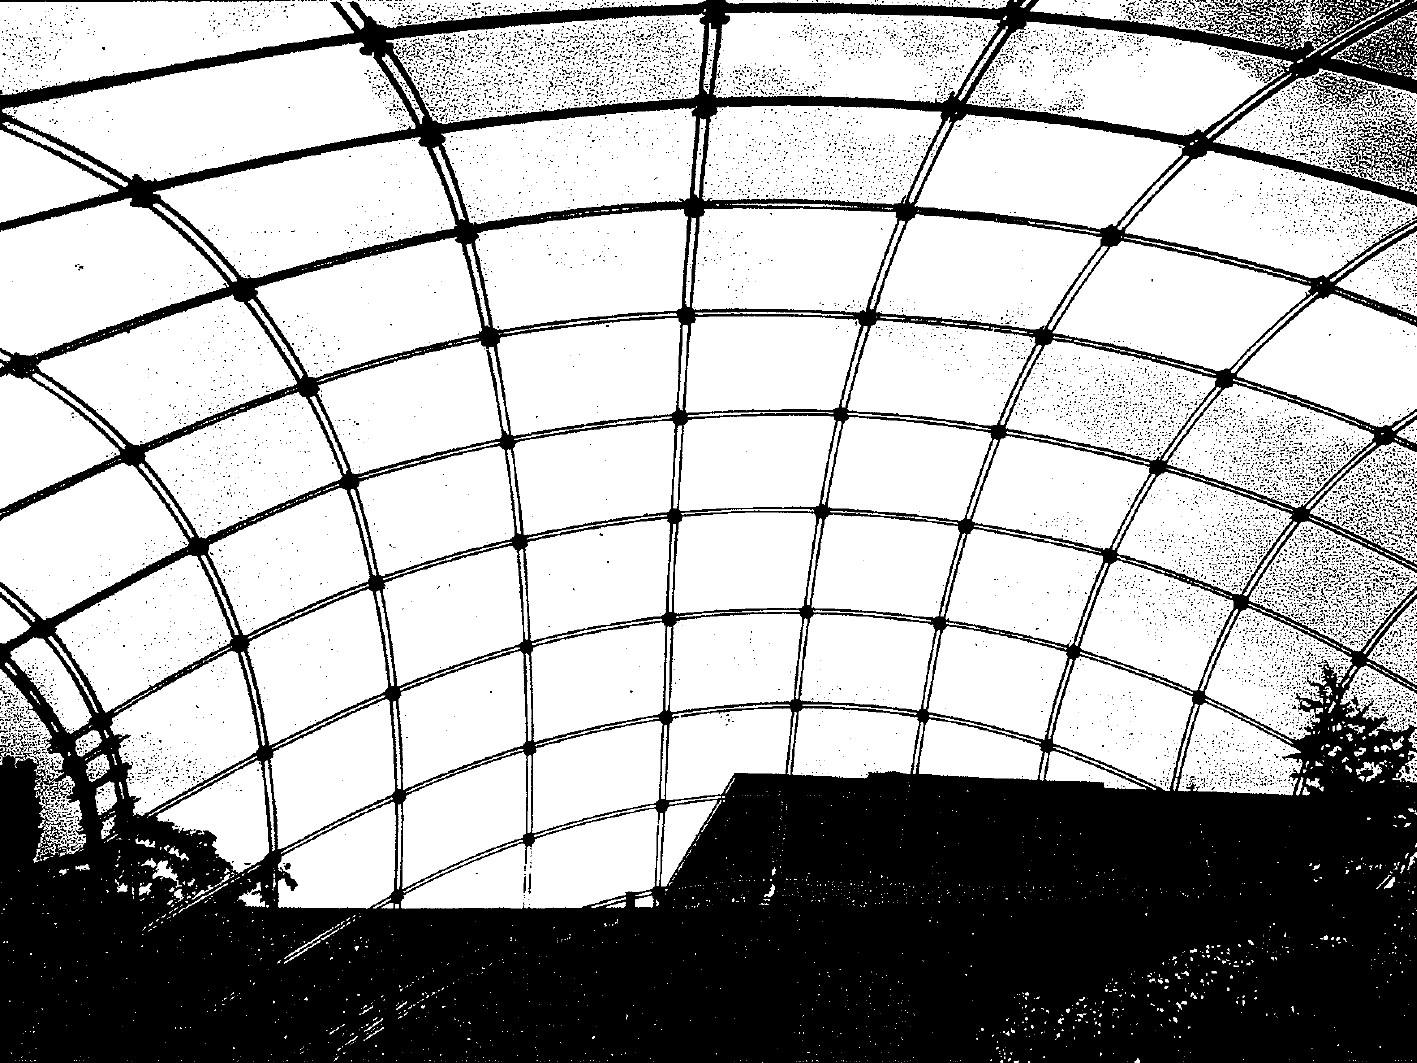
\includegraphics[width=0.48\textwidth]{berkeley_gs.jpg}\label{fig:berkeley_b}}
		\vspace{10pt}
		\captionof{figure}[Steel gridshell built in 1962 in Berkeley, USA]{Steel gridshell built in 1962 in Berkeley, USA.}
		\label{fig:berkeley}
		%
		\vspace{0.5cm}
		%
		\subfloat[][Timber lattice]{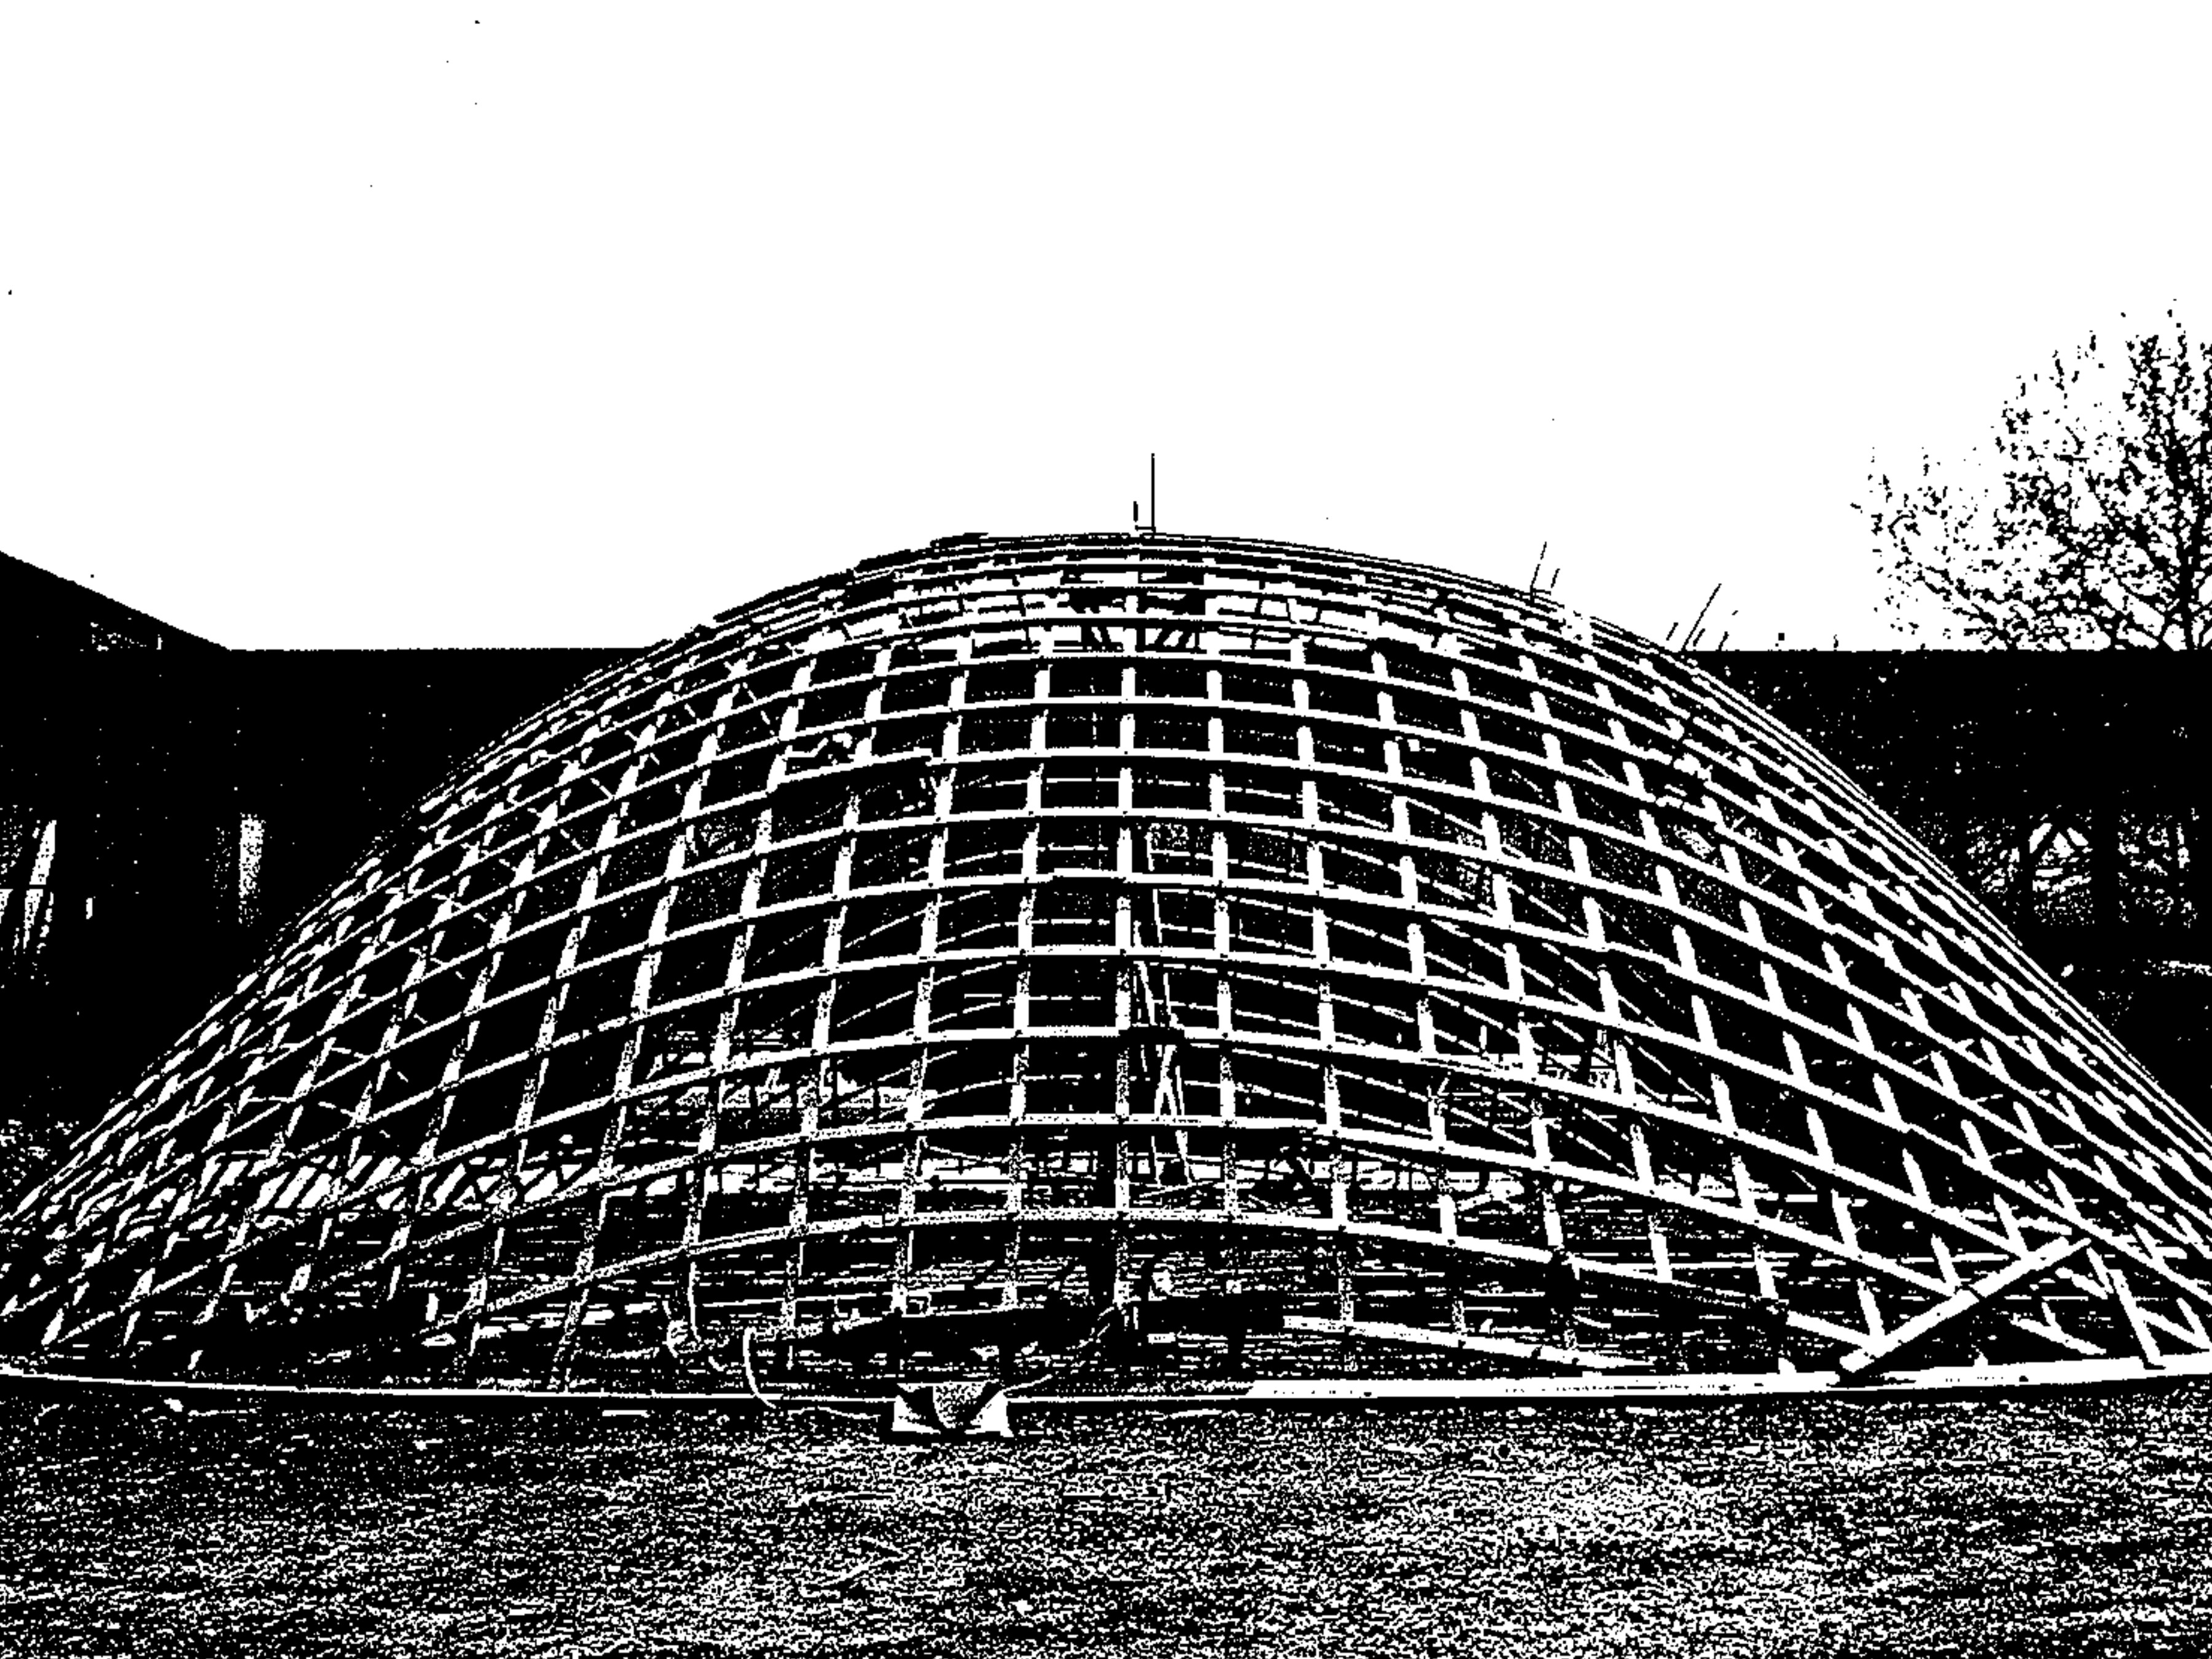
\includegraphics[width=0.48\textwidth]{essen_gs.jpg}\label{fig:essen_a}}
		\hspace*{\fill}
		\subfloat[][Plastic foil]{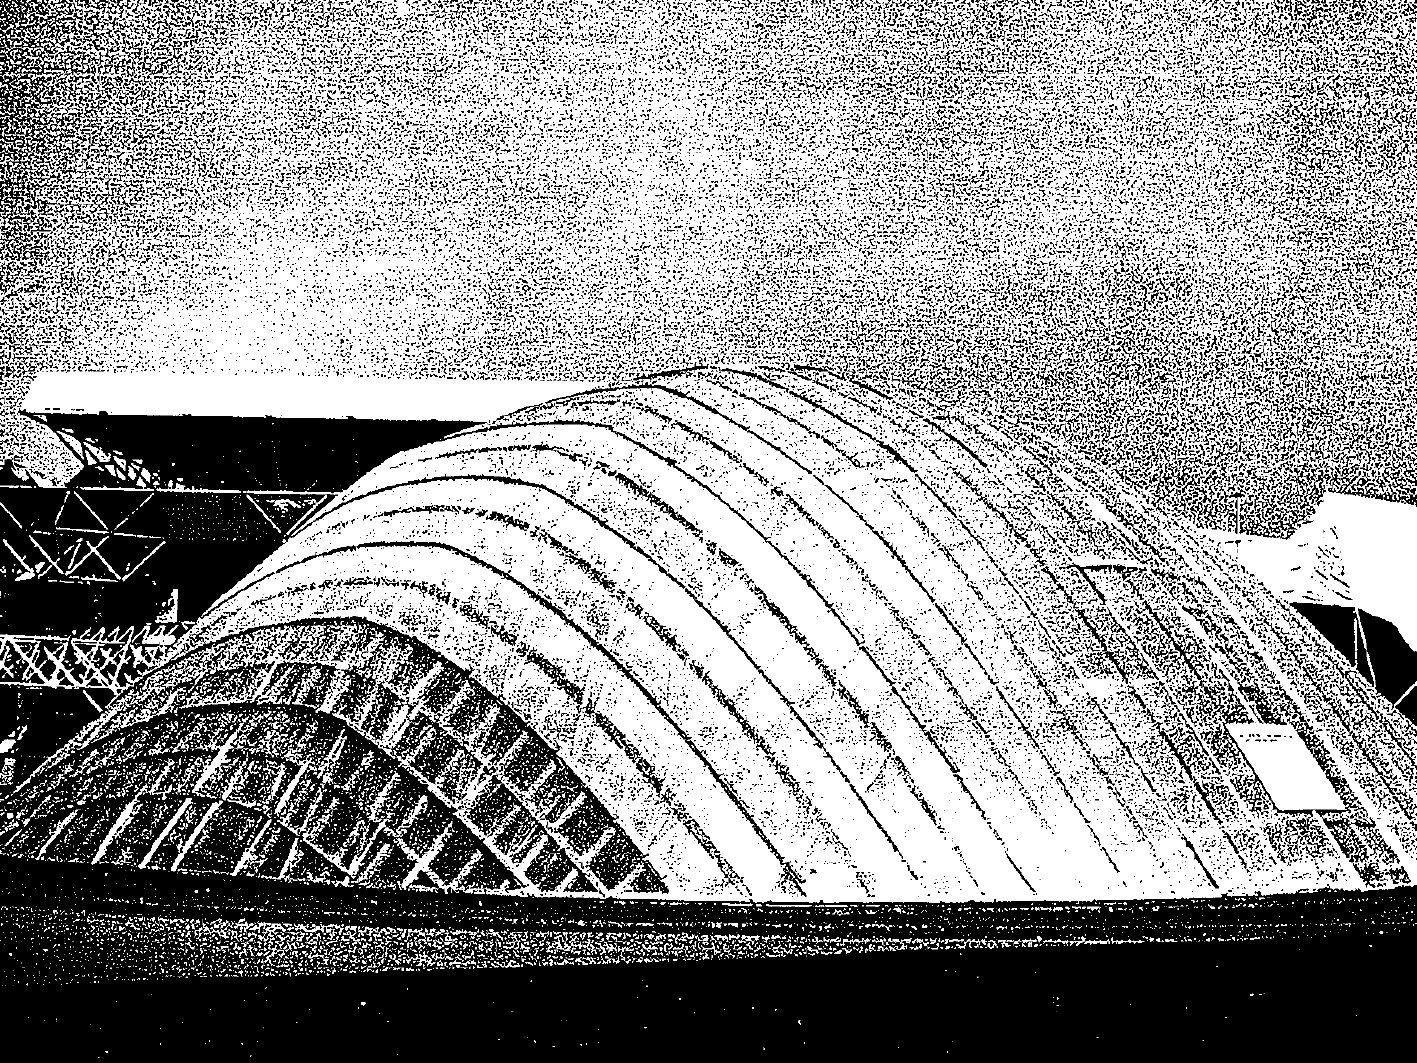
\includegraphics[width=0.48\textwidth]{essen_foil.jpg}\label{fig:essen_b}}
		\vspace{10pt}
		\captionof{figure}[Timber gridshell built in 1962 in Essen, Germany]{Timber gridshell built in 1962 in Essen, Germany.}
		\label{fig:essen}
		%
		\vspace{0.5cm}
		%
		\subfloat[][Grid erection]{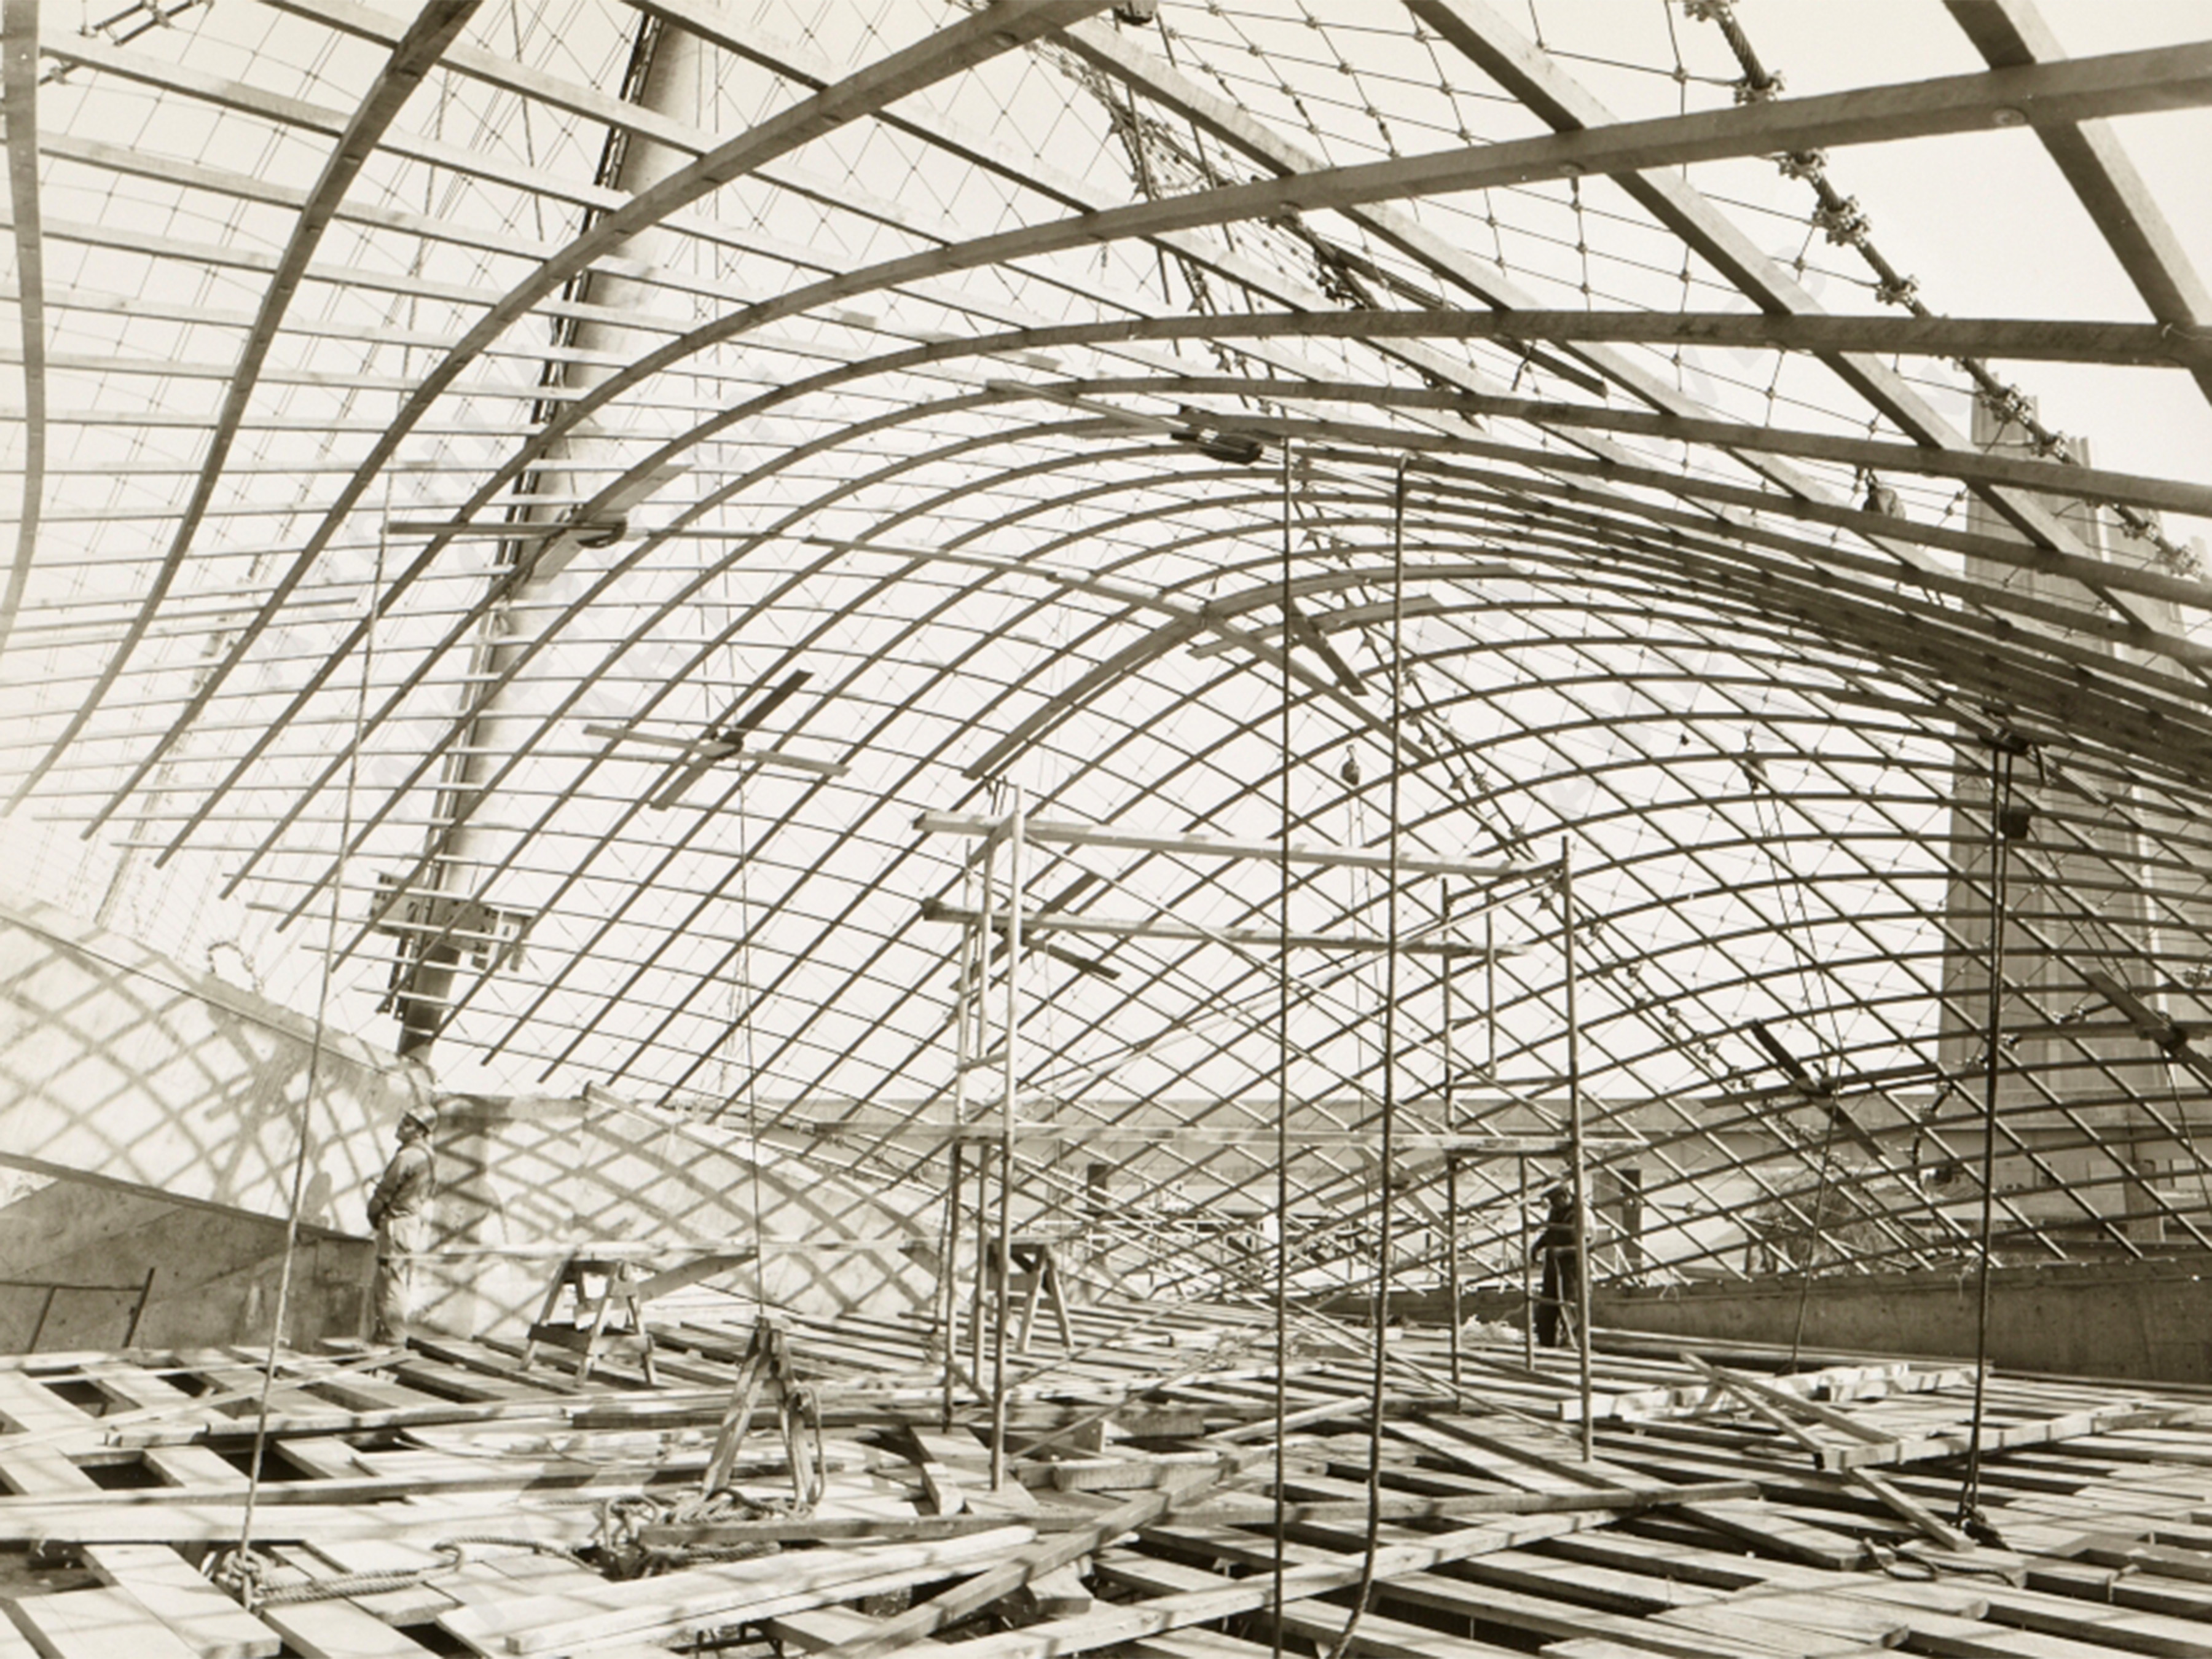
\includegraphics[width=0.48\textwidth]{montreal_lift.jpg}\label{fig:montreal_a}}
		\hspace*{\fill}
		\subfloat[][Interior view]{\includegraphics[width=0.48\textwidth]{montreal_int.jpg}\label{fig:montreal_b}}
		%
		\vspace{10pt}
		\captionof{figure}[Timber gridshell built in 1967 in Montreal, Canada]{Timber gridshell built in 1967 in Montreal, Canada.}
		\label{fig:montreal}
	\end{fullpage}
\end{figure}

\subsubsection{German Pavilion Auditoria, Montreal, Canada, 1967}
Five years later, on the occasion of the \emph{1967 International and Universal Exposition} in Montreal, Canada, Frei Otto was appointed to design the German Pavilion~: a large cable net tent prefiguring the realisation of the olympic stadium of Munich, Germany, in 1972.\footnote{Actually, Frei Otto became the director of the newly founded \emph{Institute for Lightweight Structures} (Institut für Leichte Flächentragwerke or IL) at the University of Stuttgart in 1964. It was the IL that was commissioned by the German government to conduct research in connection with the planning of the German pavilion for the exposition in Montreal.}\textsuperscript{,}\footnote{Video of the construction of the German pavilion~: \url{https://www.youtube.com/watch?v=Z0mtFMoseUk}.}

The pavilion required two auditoria and these were designed using the principle of elastic gridshell \cite[p.~274]{IL10}. All together, the auditoria covered and area of \SI{365}{m^2} and spanned \SI{17.5}{m}. The construction technique employed in Montreal was quite similar to the one developed in Essen, but this time the grid was fully braced with a layer of nailed plywood boards and offered a proper roofing made out of insulation panels covered with a PVC coated fabric (see \cref{fig:montreal_a,fig:montreal_b}).

The two gridshells built in Montreal mark a significant step in the maturation process of the technique leading to the major realisation of Mannheim in 1976~: a methodology has emerged to progress \blockcquote[p.~179]{IL10}{from the inverted form to the gridshell} ; main construction details have been validated ; various erection methods have been tested ; mid-scale buildings have been built to host public. However, due to the over complexity of these structures, lots of unknowns remained unsolved at this stage and the behaviour of the structures could not be fully predicted.\footnote{\blockcquote[p.~219]{IL10}{Snow accumulations in the throat of the common edge beam probably caused one of the two grid shells of project Montreal to buckle in a relatively flat region. The diameter of the buckled area was about 3 meters. Neither grid rod was broken, i.e. the buckling progressed elastically. It might have been possible to press the buckled area back into shape.}}

It is worthwhile to mention that several unexecuted large-scale projects were studied by Frei Otto between 1967 and 1973 at the \emph{IL} or at the \emph{Atelier Warmbronn}.\footnote{Atelier Warmbronn is the architectural studio founded by Frei Otto in 1969.} These projects are basically documented in \cite[pp.~278 - 288]{IL10} and reveal that he was training his capacity to master large-scale projects with the technique of elastic gridshells for more conventional building projects (wave pool, swimming hall, multi-purpose hall, auditorium, \telp{}).

\subsection{Mannheim Multihalle : the completion of a decade of research}
The project of the Multihalle started in 1970, when the decision was made that Mannheim, Germany, would hold the Bundesgartenschau in 1975.\footnote{The Bundesgartenschau is a national horticultural exhibition that takes place every two years in Germany.} The architects of the project, \emph{Carl Mutschler \& Partners}, consulted Frei Otto at \emph{Atelier Warmbronn} as he was starting to get known in the filed of innovative lightweight structures. This is how the idea of the gridshell was introduced in the project \cite{Liddell2015}.

A thorough report on the project is available in \cite{IL13}.  A more condensed but still precise description of the engineering problematics related to this project are available in the excellent papers from \citet{Happold1975, Liddell2015}.

\subsubsection{Multihalle, Mannheim, Germany, 1975}
Mannheim is an unprecedented realisation because it is more than twenty times larger than the previously built gridshells in Montreal and is meant to last many years and not only for the duration of a short-term exhibition. The timber lattice, still existing in 2017,  covers an area of \SI{7400}{m^2} (see \cref{fig:mannheim_b}). It is composed of two interconnected domes, one for the multi-purpose hall (span : \SI{60}{m} | height : \SI{20}{m}) and one for the restaurant (span : \SI{50}{m} | height : \SI{18}{m}).

Although the constructive system deployed in Mannheim clearly inherited from the previous developments, the challenge was such that it had to be revisited. In particular the main additions were the introduction of the double-layer system and the proper bracing of the grid. A major advance was also the use of the very first numeric models to study the structure.

The double-layer system was introduced to tackle two issues~: the grid needed some flexibility to be bent into the desired shape, but once erected it should provide sufficient bending stiffness to resist disturbing loads and avoid a buckling collapse.\footnote{Theoretically, self-weight loads would produce only compression in the members because the (funicular) form of the grid resulted from the inversion of a hanging chain model in pure tension.} Once erected, the two grids, one sliding on top of the other one, were connected together to form a single grid with much higher ladder profiles (from \SI{50}{mm} to \SI{150}{mm}), increasing their bending stiffness by a factor of about 26 (see \cref{fig:mannheim_a}).
\begin{figure}[t]
		\subfloat[][Interior view]{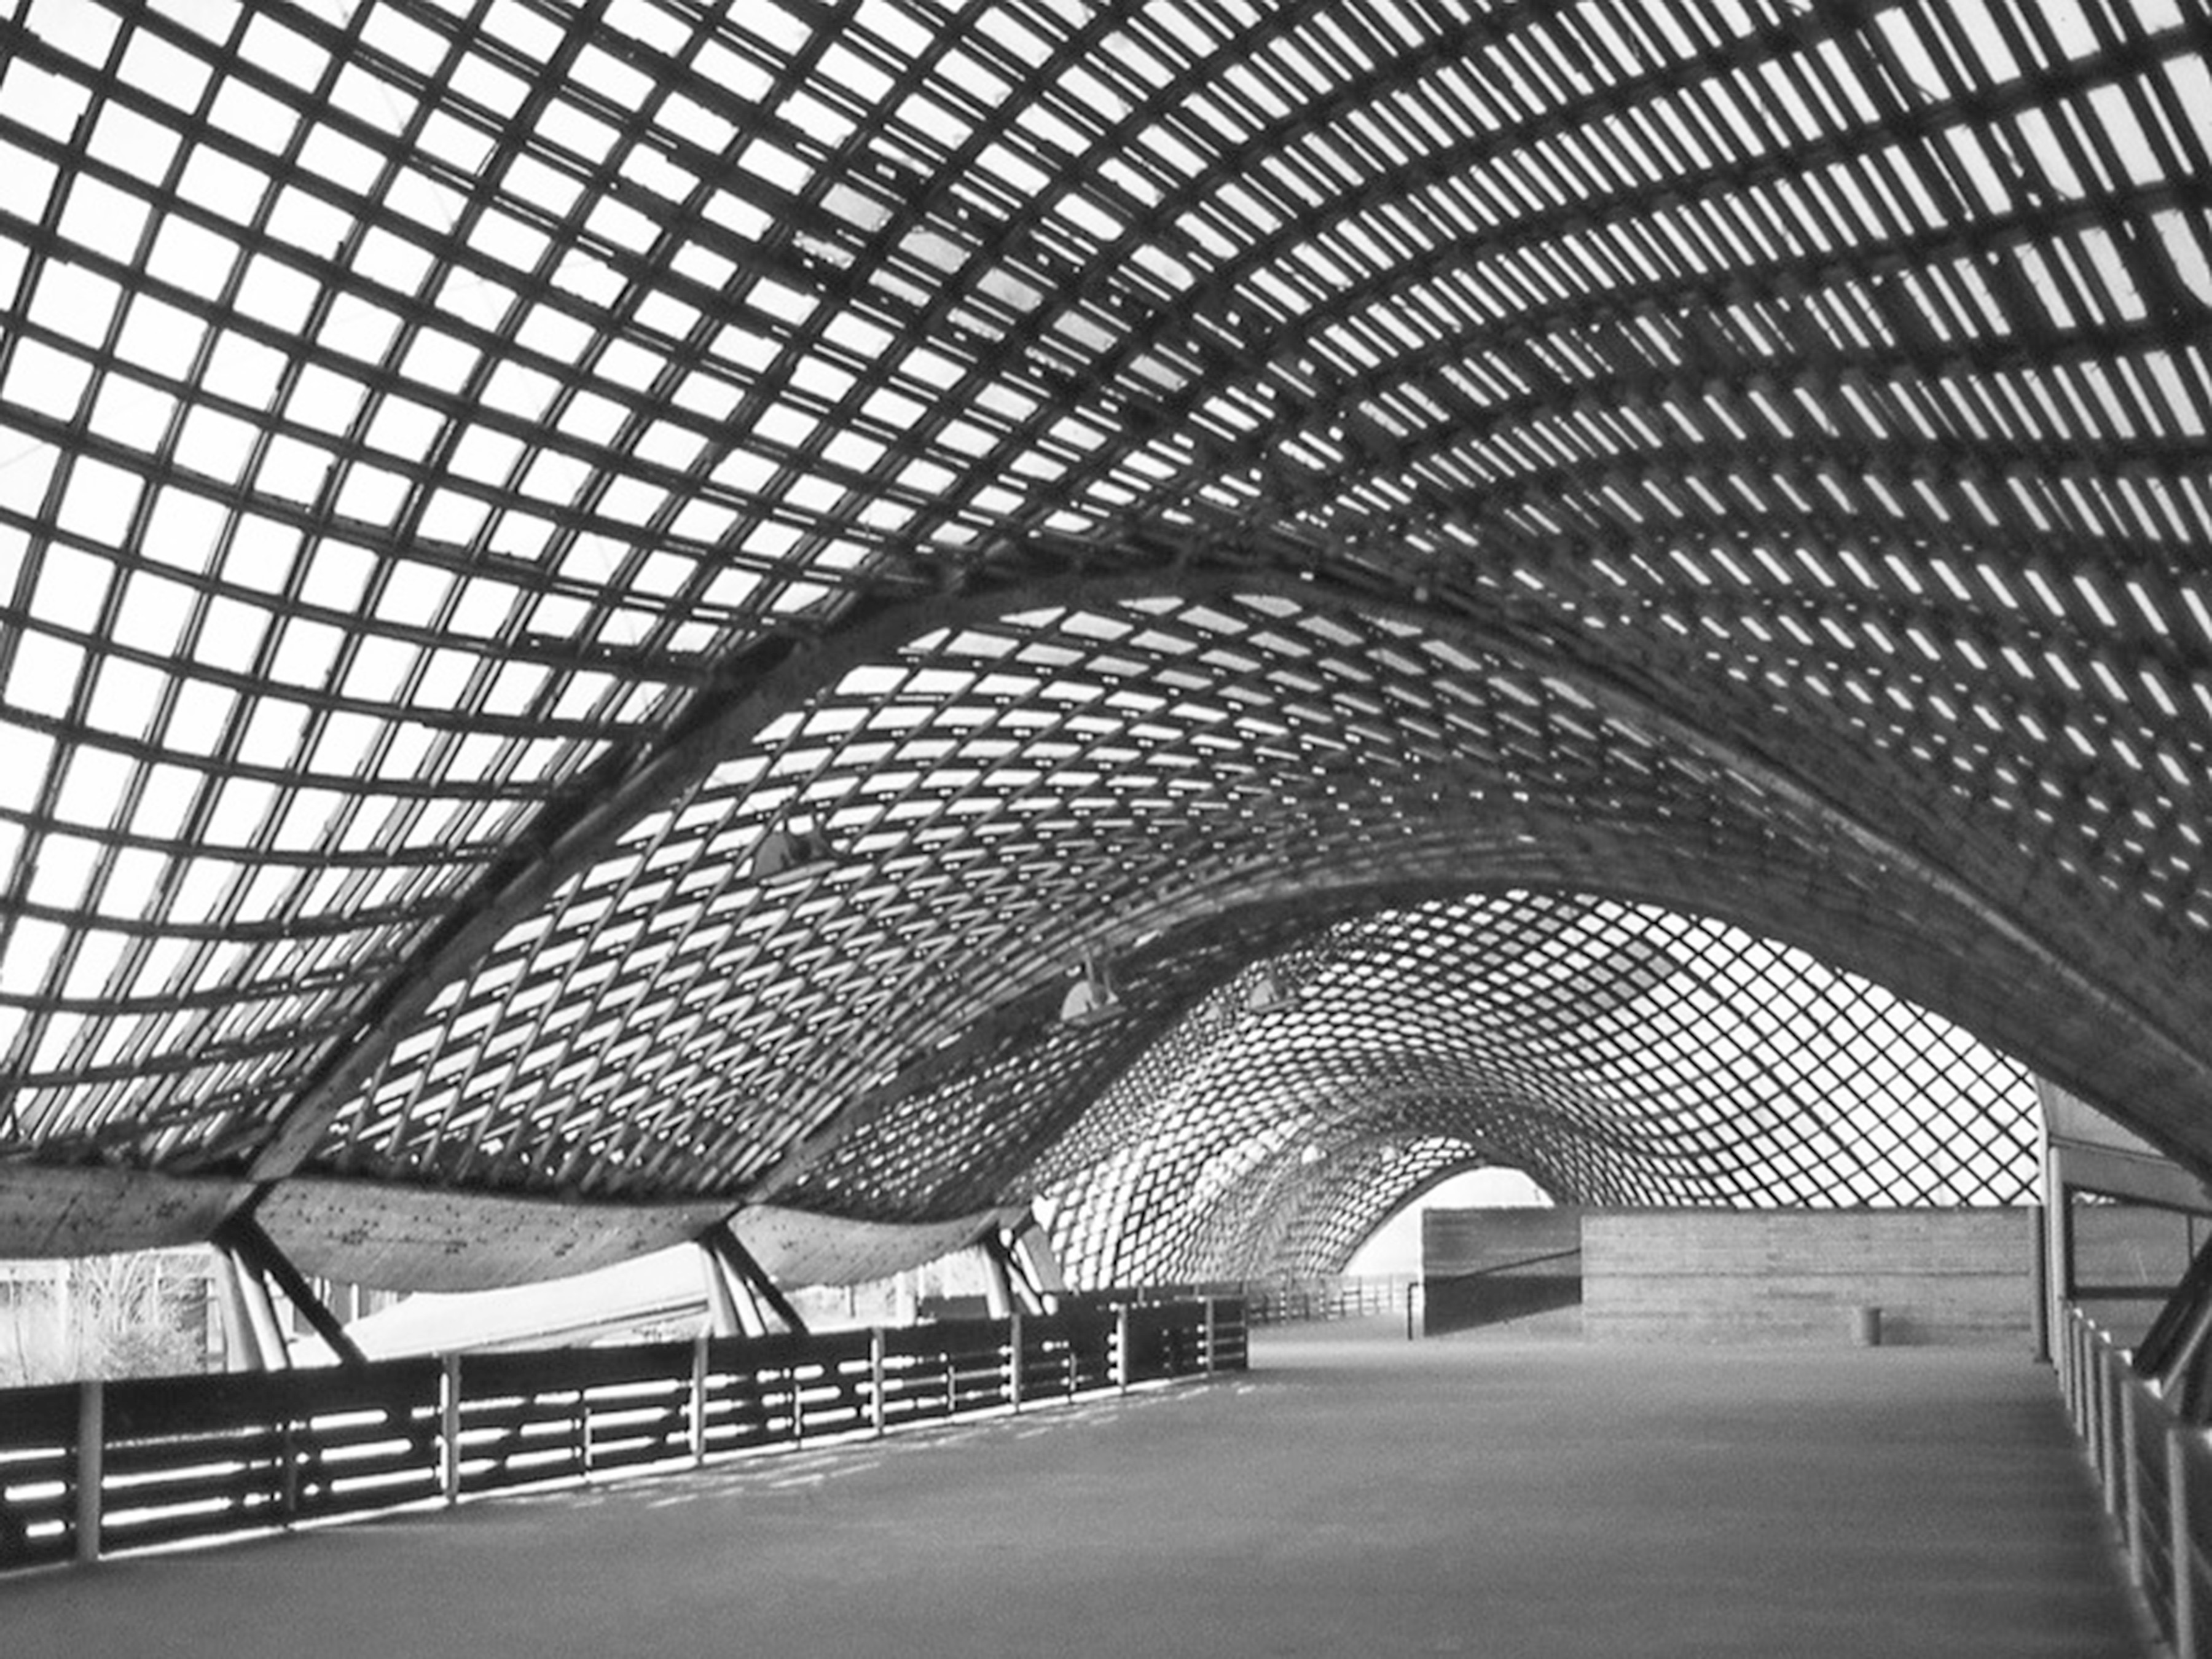
\includegraphics[width=0.48\textwidth]{mannheim_int.jpg}\label{fig:mannheim_a}}
		\hspace*{\fill}
		\subfloat[][Sky view]{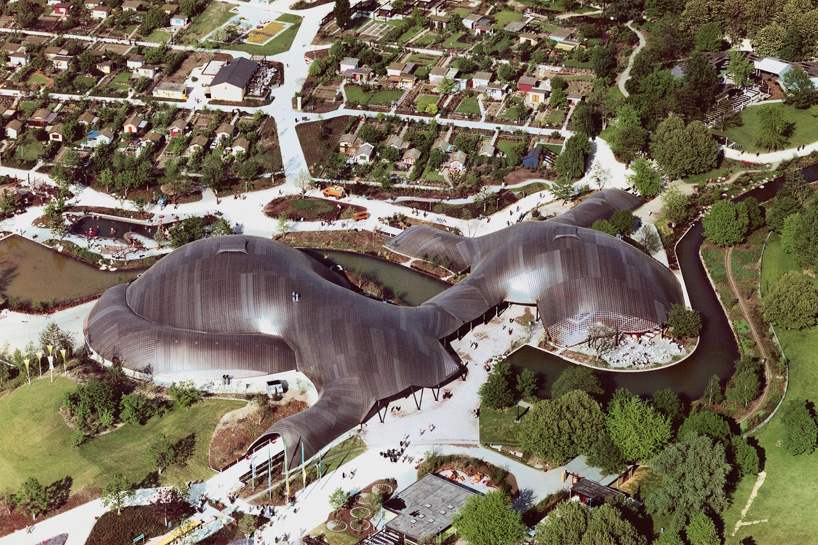
\includegraphics[width=0.48\textwidth]{mannheim_sky.jpg}\label{fig:mannheim_b}}
		%
		\vspace{10pt}
		\captionof{figure}[Timber gridshell built in 1962 in Essen, Germany]{Timber gridshell built in 1975 in Mannheim, Germany.}
		\label{fig:mannheim}
\end{figure}

Because the in-plane stiffness of the grid also plays a major role in the resistance to buckling, this question was considered with care. The bracing of the grid was first achieved by preventing the nodes to turn once the grid was erected. This was done by creating some friction in the nodes when tightening the bolts linking the laths, after the grid was erected. Then, additional bracing cables were put in the grid.

Finally, the project of Mannheim was a key project in the development of modern lightweight structures. Great engineers were born in touch with Frei Otto, following his footsteps or collaborating with him. This heritage has irrigated for several decades the engineering of lightweight structures in Europe and gave birth, directly or indirectly, to several studios among which we can cite \emph{Buro Happold} and \emph{Schlaich Bergermann \& Partner}.

\subsection{The dry period : 25 years from Mannheim to Hannover}

Although the experience of Mannheim proved the feasibility and the potential of gridshell structures for large-scale projects, it also revealed that these projects were subject to an incredible complexity in terms of structural design, geometry, modelling, testing, team work, construction methods \telp{} At that time, very few people could pretend to master all the knowledge and techniques required to design and built timber gridshells and developed in the bosom of the \emph{Institute for Lightweight Structures} in Stuttgart.

This project was obviously well ahead of its time and the engineering cost to design such structures was probably prohibitive considering the tools available at that time. This certainly explains why no elastic gridshells were built during the 25 following years, despite the optimism of the pioneers of the Multihalle.\footnote{\blockcquote[]{Harris2003}{For many years after its completion, Happold promoted the benefit of the timber gridshell as a construction technique and stated that he could not understand why it had not been adopted more widely. He perceived the benefits to be in the efficiency of the construction method to enable doubly curved (shell) structures to be constructed quickly and cost effectively.}.}

Note that around 1975 small workshop and experiments lead to the construction of several but small elastic gridshells, as reported in \cite{IL10}. A non-exhaustive but quite extensive list of known executed gridshell projects is presented in \cref{fig:projectsbymaterial}. The dry period is clearly visible.

\subsection{The signs of a renewal : Dorset and Doncaster}\label{sec=signs}

It is only 20 years later that gridshells started to reappear, in the late 90's mainly in the United Kindom, and for projects that had interest in environmental problematics.

\subsubsection{Westminster Lodge, Dorset, England, 1995}
In 1995, a small student residence named \emph{Westminster Lodge} was built in Dorset, England. This dwelling was part of a larger project -- Hooke Park -- aiming at investigating how the local forest resources, in particular immature roundwood thinnings, could be better utilised. The project was lead by ABK, Frei Otto, Buro Happold and Cullinan Studio. Unlike Mannheim, the timber shell was bent and weaved rod by rod on a scaffold platform. But the structural system exhibited a double-layer gridshell pattern very similar to the one employed for the Multihalle (see \cref{fig:dorset_a}). The rods were made out of splice-jointed roundwood to form long-length poles of diameter \SI{200}{mm}. The development of this jointing technique, which could be produced directly in the forest, was part of the project's investigations \cite{Burton1998}. The grid was braced by a layer of diagonal boards nailed to the roundwood. The structure was finally cladded with a planted turf roof (see \cref{fig:dorset_b}).

\subsubsection{Earth Center, Doncaster, England, 1998}
At the same time, a project with a similar spirit arose for the \emph{Earth Center} in Doncaster, England.\footnote{\textquote{\href{http://grant-associates.uk.com/approach/earth-centre-forest-garden-grid-shells/}{The Earth Centre Forest Garden} was intended to demonstrate how managed woodland could supply the vast majority of all natural resources needed for human survival.}} The project planning started in 1994 and a series of small timber gridshells were designed by Buro Happold and then built in 1998. The landscape structures were single-layer timber gridshells made with oak laths. Once erected with a crane, the grids were braced with crossing diagonal stainless steel cables (see \cref{fig:doncaster_a}). Openings were possibly reinforced with curved timber frames (see \cref{fig:doncaster_b}).

These projects definitely trailed the technique in England and initiated the renewal period (see \cref{sec=renewal}). Although they remained small-scale projects for which modelling was achieved through physical models, they trained and restored partially the operational ability of Buro Happold to design timber gridshells as pointed by \citet{Harris2003}.

\begin{figure}[t]
     	\centering
%	\begin{fullpage}
		\subfloat[][Interior view]{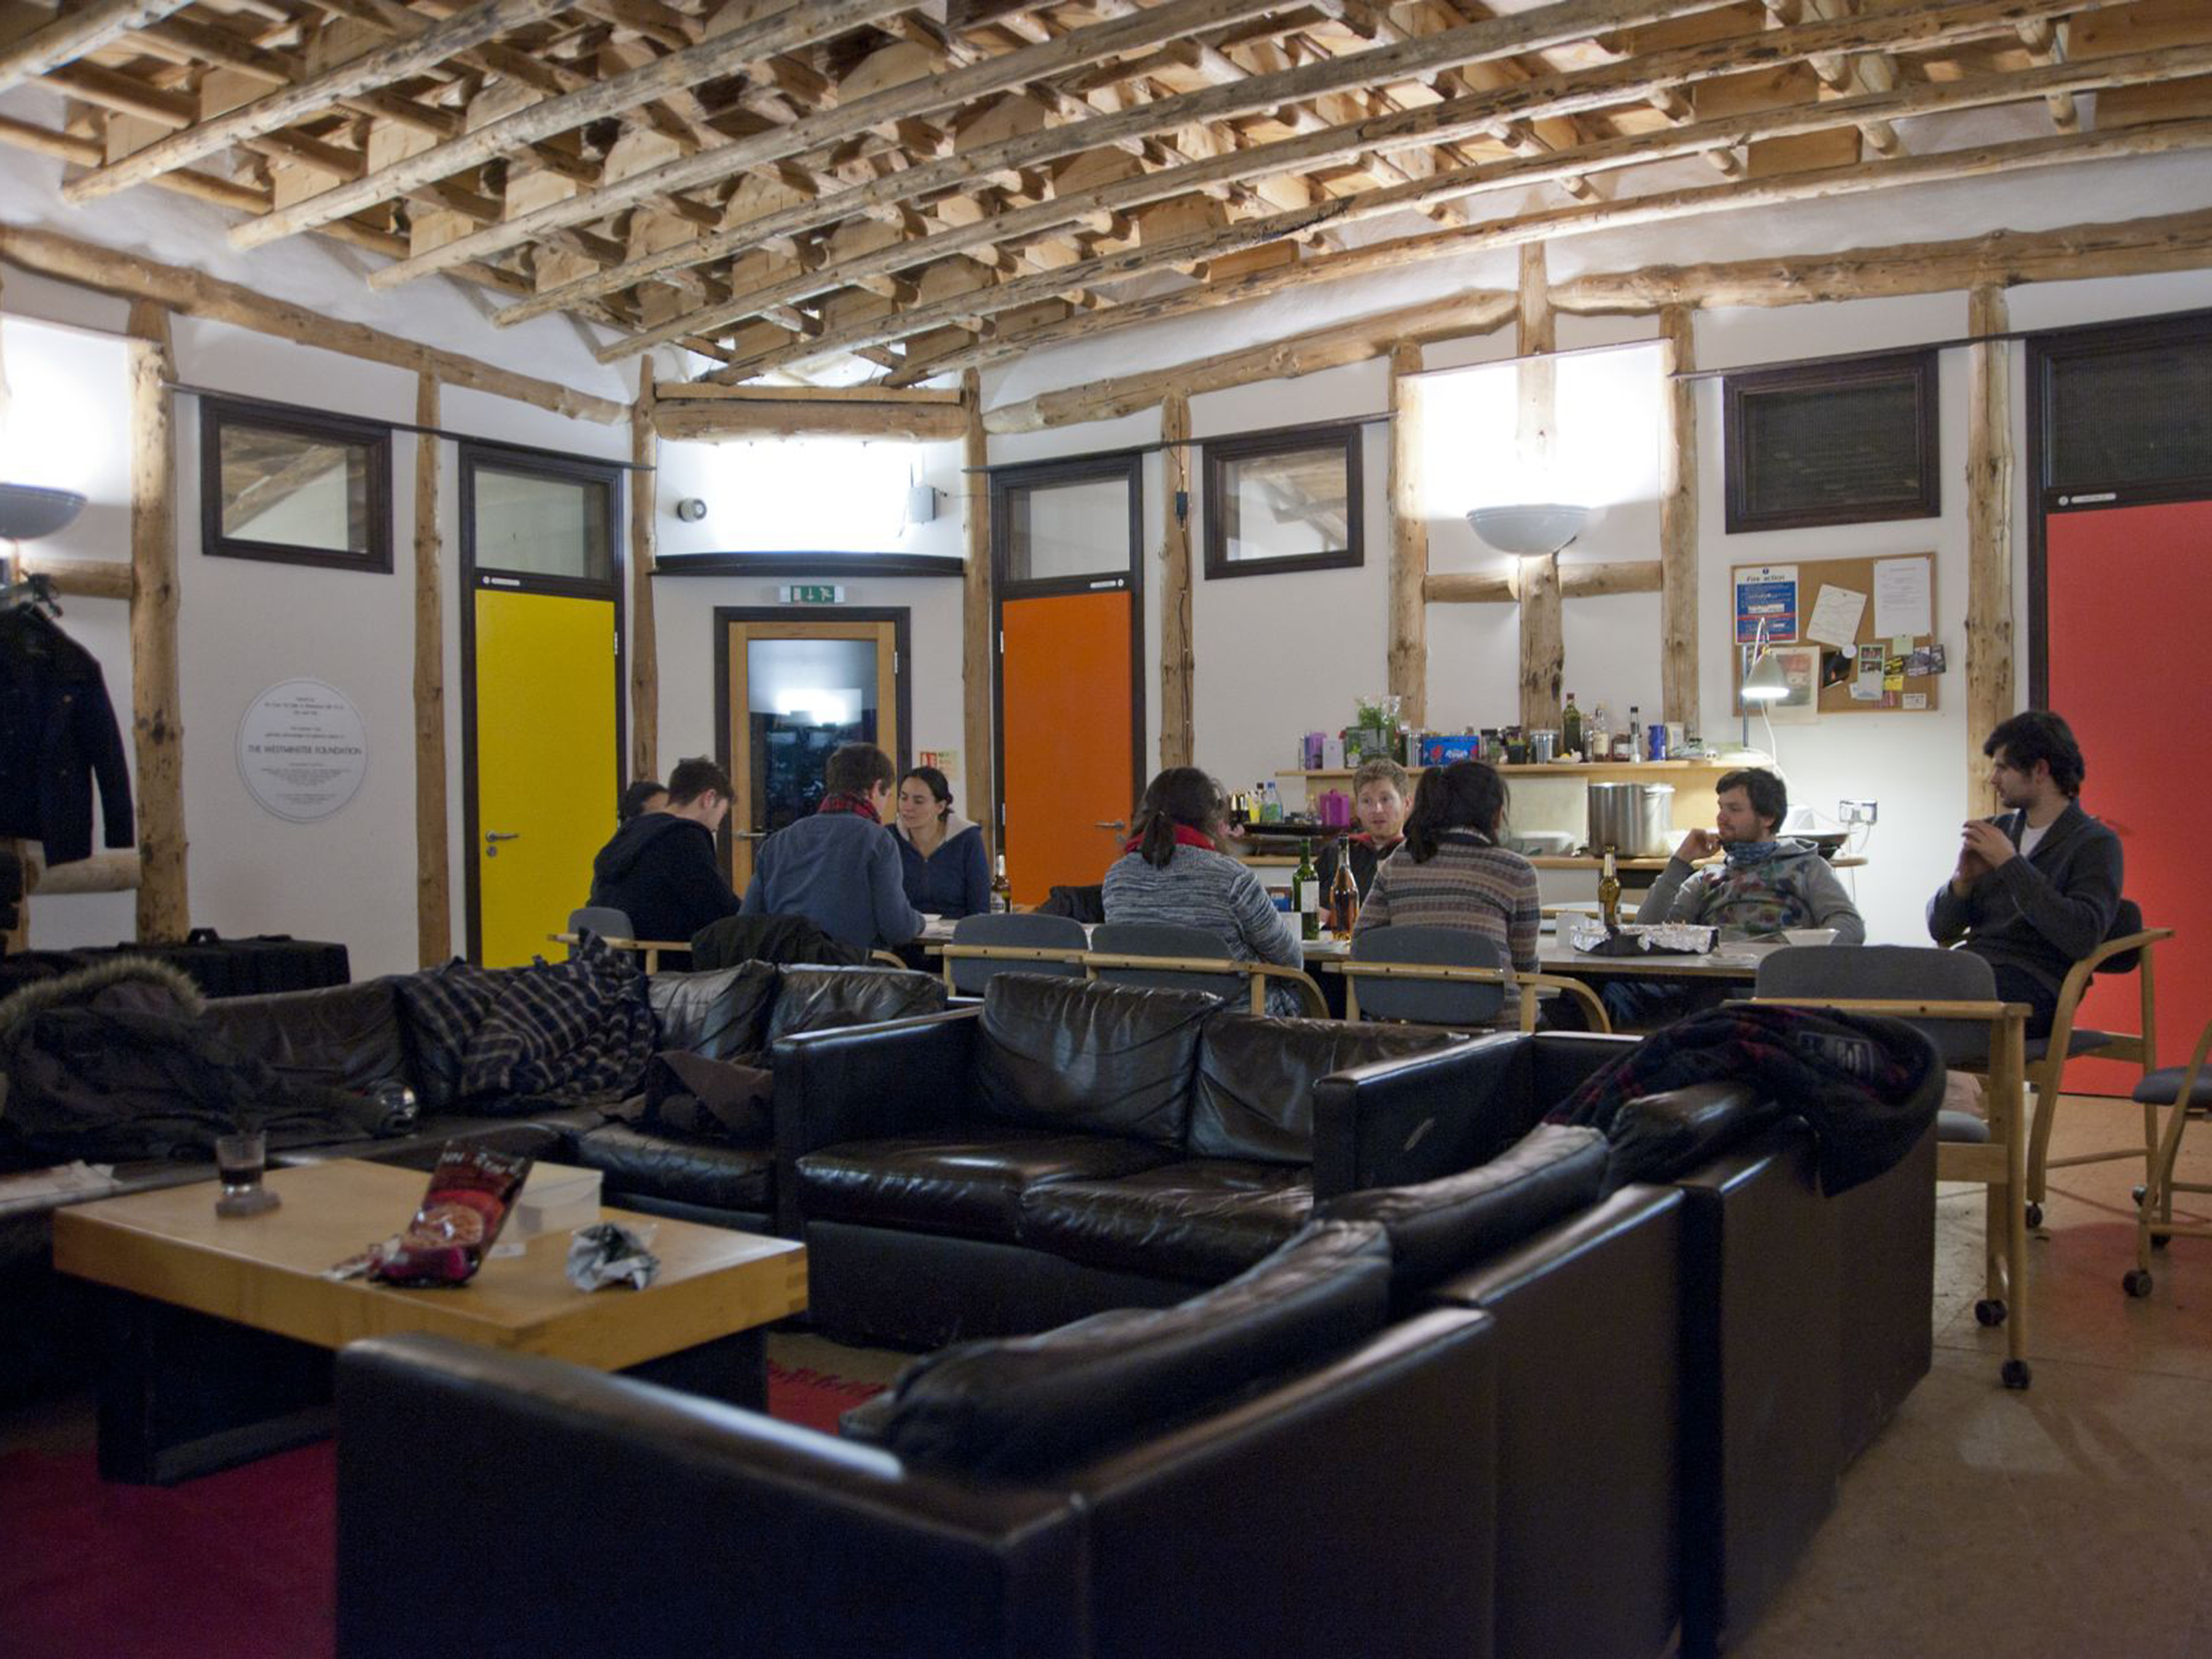
\includegraphics[width=0.48\textwidth]{dorset_int.jpg}\label{fig:dorset_a}}
		\hspace*{\fill}
		\subfloat[][Exterior view]{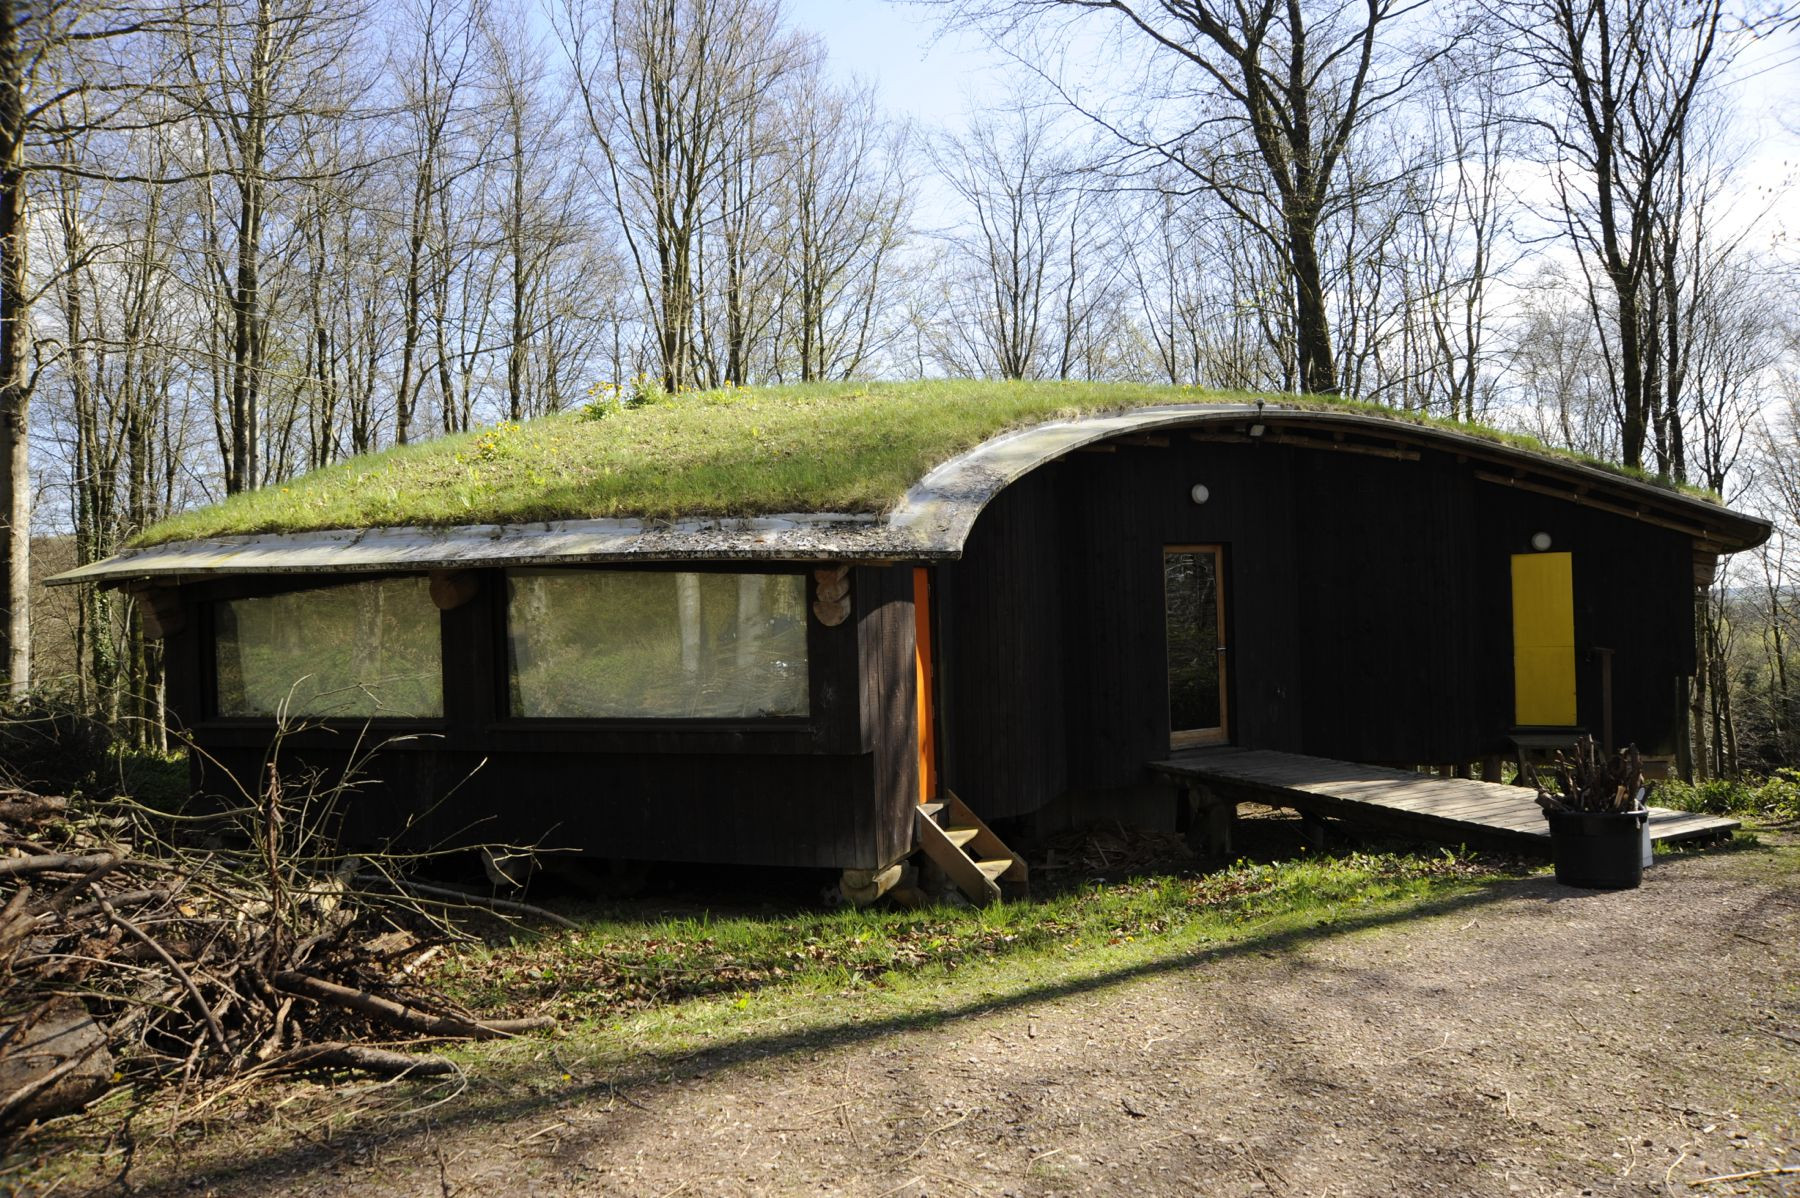
\includegraphics[width=0.48\textwidth]{dorset_ext.jpg}\label{fig:dorset_b}}
		\vspace{10pt}
		\captionof{figure}[Roundwood gridshell built in 1995 in Dorset, England]{Roundwood gridshell built in 1995 in Dorset, England.}
		\label{fig:dorset}
		%
		\vspace{0.5cm}
		%
		\subfloat[][Interior view]{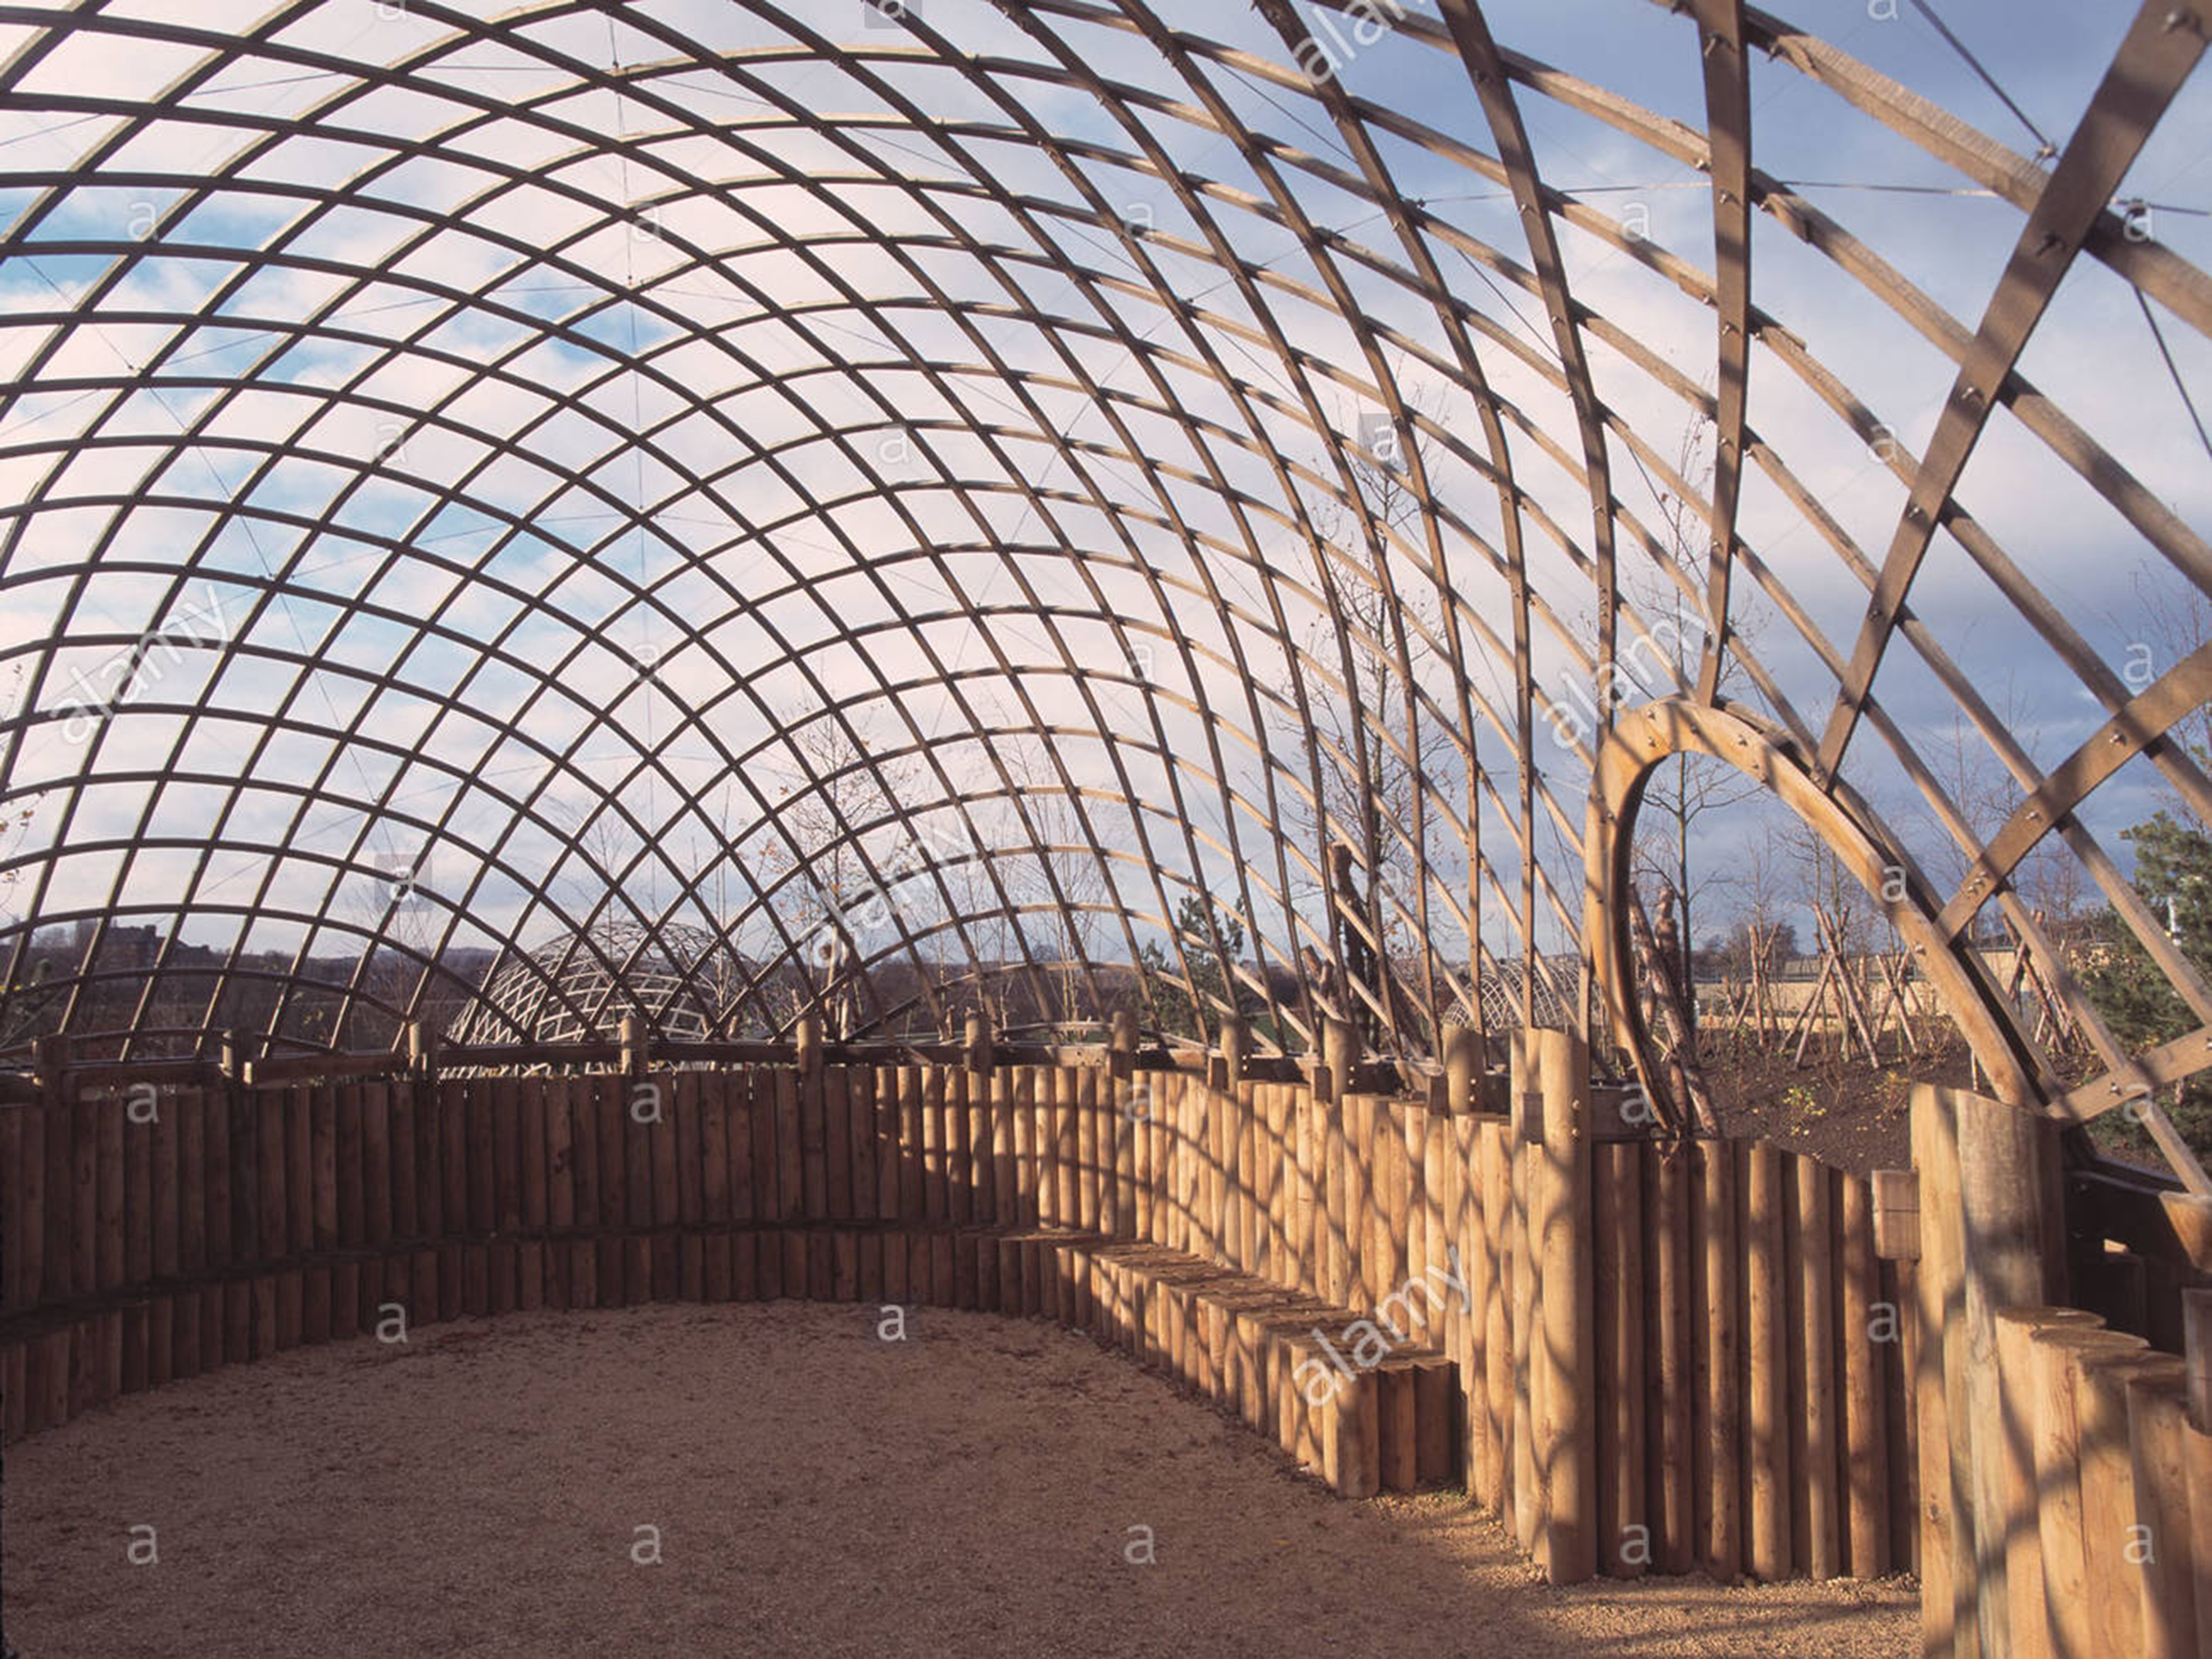
\includegraphics[width=0.48\textwidth]{doncaster_int.jpg}\label{fig:doncaster_a}}
		\hspace*{\fill}
		\subfloat[][Exterior view]{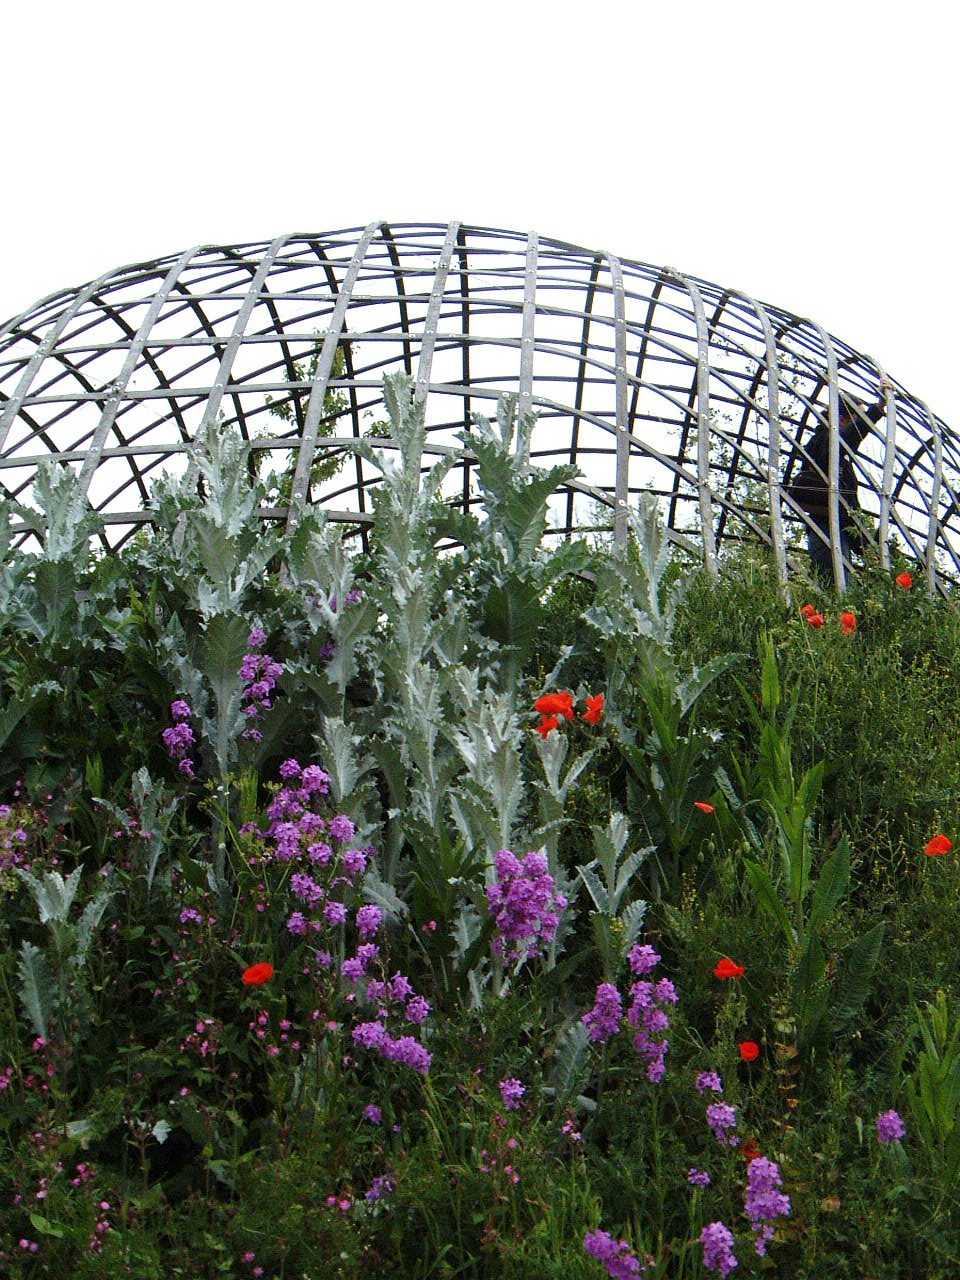
\includegraphics[width=0.48\textwidth]{doncaster_ext.jpg}\label{fig:doncaster_b}}
		\vspace{10pt}
		\captionof{figure}[Timber gridshells built in 1998 in Doncaster, England]{Timber gridshells built in 1998 in Doncaster, England.}
		\label{fig:doncaster}
%	\end{fullpage}
\end{figure}

\subsection{The renewal : Hannover, Downland and Savill}
\label{sec=renewal}

What was missing for elastic gridshells to re-emerge after the major experiment of Mannheim was probably the development of modern numeric tools to ease and speed up the design process.\footnote{\blockcquote[]{Harris2003}{The key to the modern use of timber gridshells is the development of computer methods in modelling complex three-dimensional shell structures. For the Mannheim structure, the primary method of form finding was the use of physical models. The Earth Centre structures were small and easily modelled using wire mesh, but when Buro Happold was commissioned to design the Japanese Pavilion for Expo 2000 in Hannover (Architect Shigeru Ban), it was apparent that much more sophisticated computer form finding and analysis would be necessary.}} Amongst those tools we should identify two main categories~: geometry processing softwares and structural analysis softwares. Recall that in the 70's, geometry processing was done through physical models and photographic measurements \cite[pp.~130-135]{IL10} while structural analysis was conducted through a compound of physical model testing with scaling techniques \cite[pp.~130-135]{IL13}, hand calculations and the very first numerical form-finding calculations \cite[pp.~184-193]{IL10} and finite element calculations \cite[pp.~210-217]{IL10}. In the late 90's, the rise in importance of computer methods offered new possibilities.

\subsubsection{Japan Pavilion, Hannover, Germany, 2000}
In 1997, architect Shigeru Ban began to collaborate with Frei Otto and Buro Happold to design the \emph{Japan Pavilion} for \emph{Expo 2000} in Hannover, Germany \cite{Ban2006}. This pavilion was a large-scale corrugated gridshell made out of cardboard tubes, about 75 meters long and 25 meters wide. Corrugations bring curvature, and therefore enhance the strength of the shell. The tubes were tied together with a fabric tape, a very low-tech joint (see \cref{fig:hannover_a}). The structure was covered with a paper membrane specially developed for the project to meet the requirements of the German fire regulations (see \cref{fig:hannover_b}). For the occasion, a new erection method was set up in which the grid was laid out not at the ground level but at a higher level on a hydraulic scaffold platform. From there, the grid was pushed up into position using the platform's jacks. It was found late that the cardboard tubes were subject to a high level of creep. This required the introduction of new timber arches to reinforce the gridshell and to enlarge the existing timber rafters intended to brace the grid and support the paper membrane (see \cref{fig:hannover_a}).

\subsubsection{Weald and Downland, Singelton, England, 2002}
The design of the \emph{Downland} gridshell began right after the completion of the Westminster Lodge (see \cref{sec=signs}) where architects from E. Cullinan Studio became acquainted with the engineers from Buro Happold. At Downland, the project team truly revived the technique of large-scale timber gridshells while bringing lots of improvements to the system. The building opened to the public in 2002. Its corrugated shape recalls the one of the Japan Pavilion from which it was inspired (see \cref{fig:downland_b}).

The building is 50 meters long and 12.5 to 16 meters wide, covering an area of about \SI{675}{m^2} for a height varying from 7 to 9.5 meters \cite{Harris2002}. The structure is a double-layer gridshell made of rectangular oak laths of cross-section \SI{50}{mm} x \SI{35}{mm} (see \cref{fig:downland_a}). To produce high grade timber elements, the continuous laths were re-formed from small carefully selected wood pieces, finger-jointed every \SI{60}{cm} in \SI{6.0}{m} length pieces. These pieces of lath were then scarf-jointed on site every \SI{6}{m} to obtained the desired length, up to \SI{50}{m}.
\begin{figure}[t]
     	\centering
%	\begin{fullpage}
		\subfloat[][Interior view]{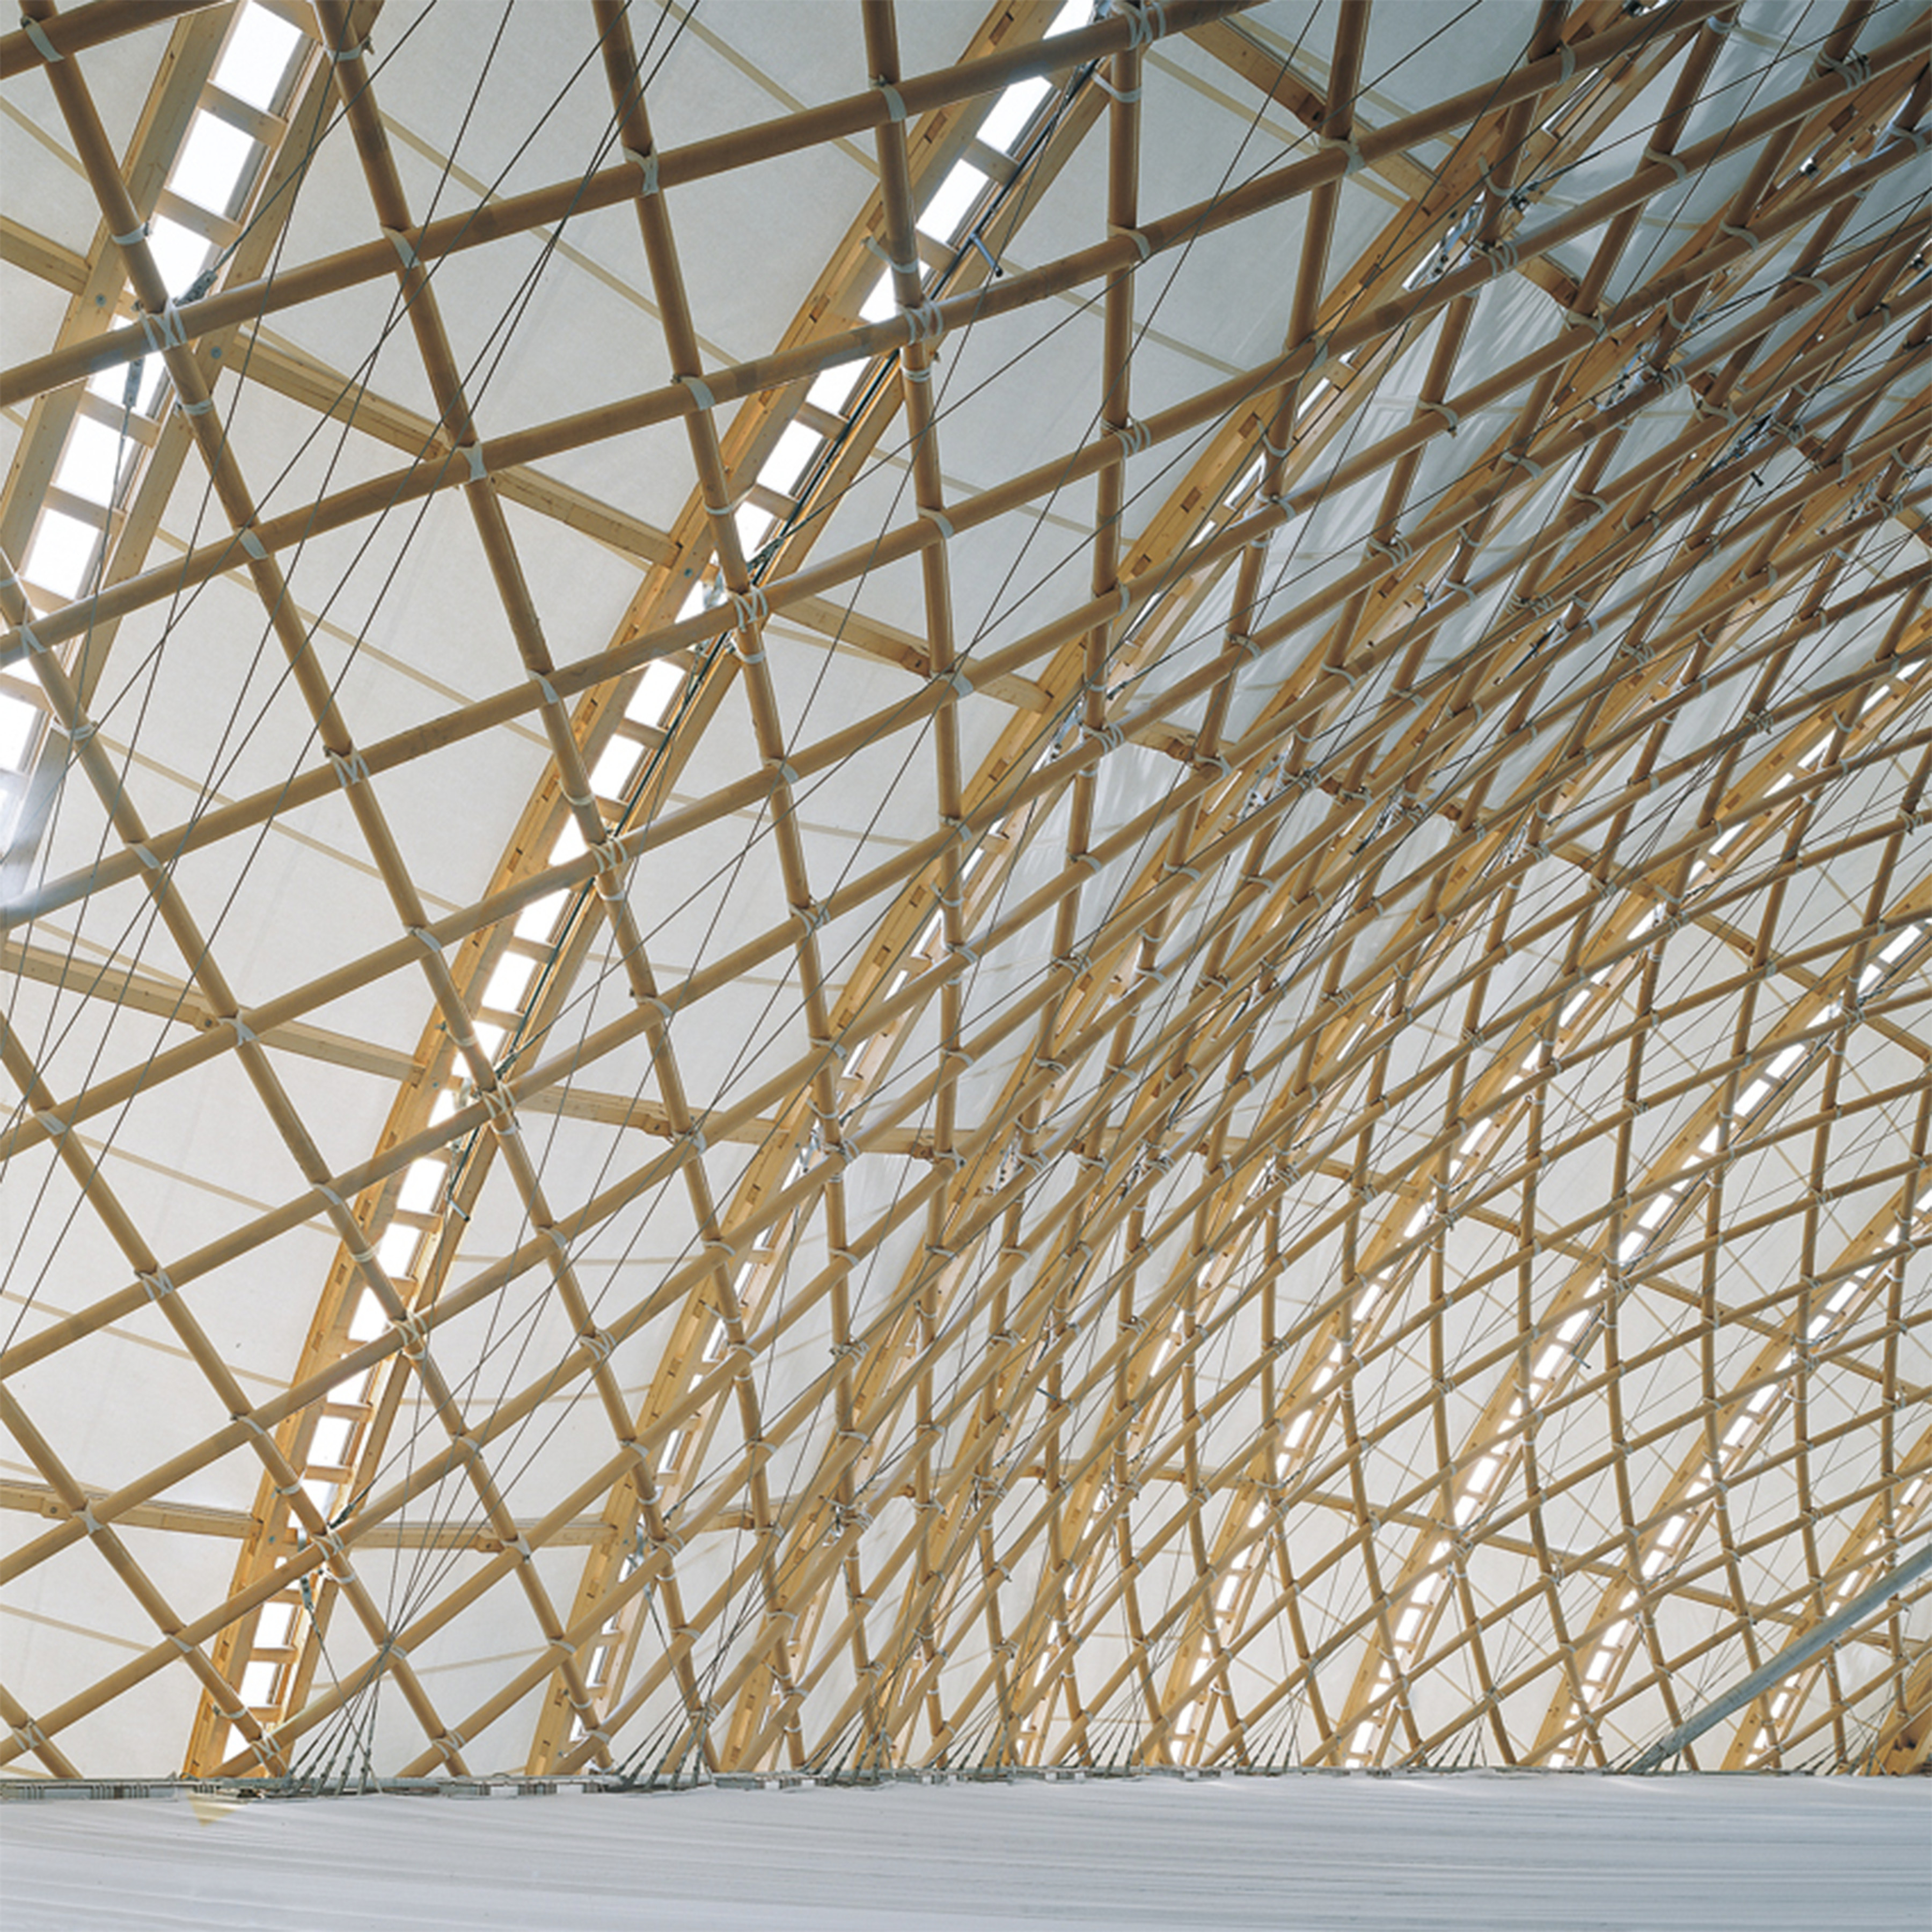
\includegraphics[width=0.32\textwidth]{hannover_int.jpg}\label{fig:hannover_a}}
		\hspace*{\fill}
		\subfloat[][Sky view]{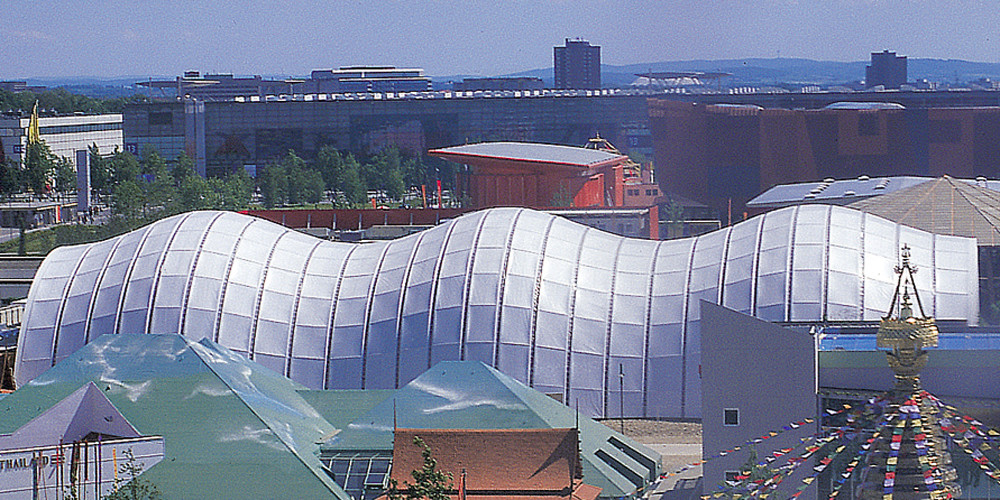
\includegraphics[width=0.64\textwidth]{hannover_sky.jpg}\label{fig:hannover_b}}
		\vspace{10pt}
		\captionof{figure}[Cardboard gridshell built in 2000 in Hannover, Germany]{Cardboard gridshell built in 2000 in Hannover, Germany.}
		\label{fig:hannover}
		%
		\vspace{0.5cm}
		%
		\subfloat[][Interior view]{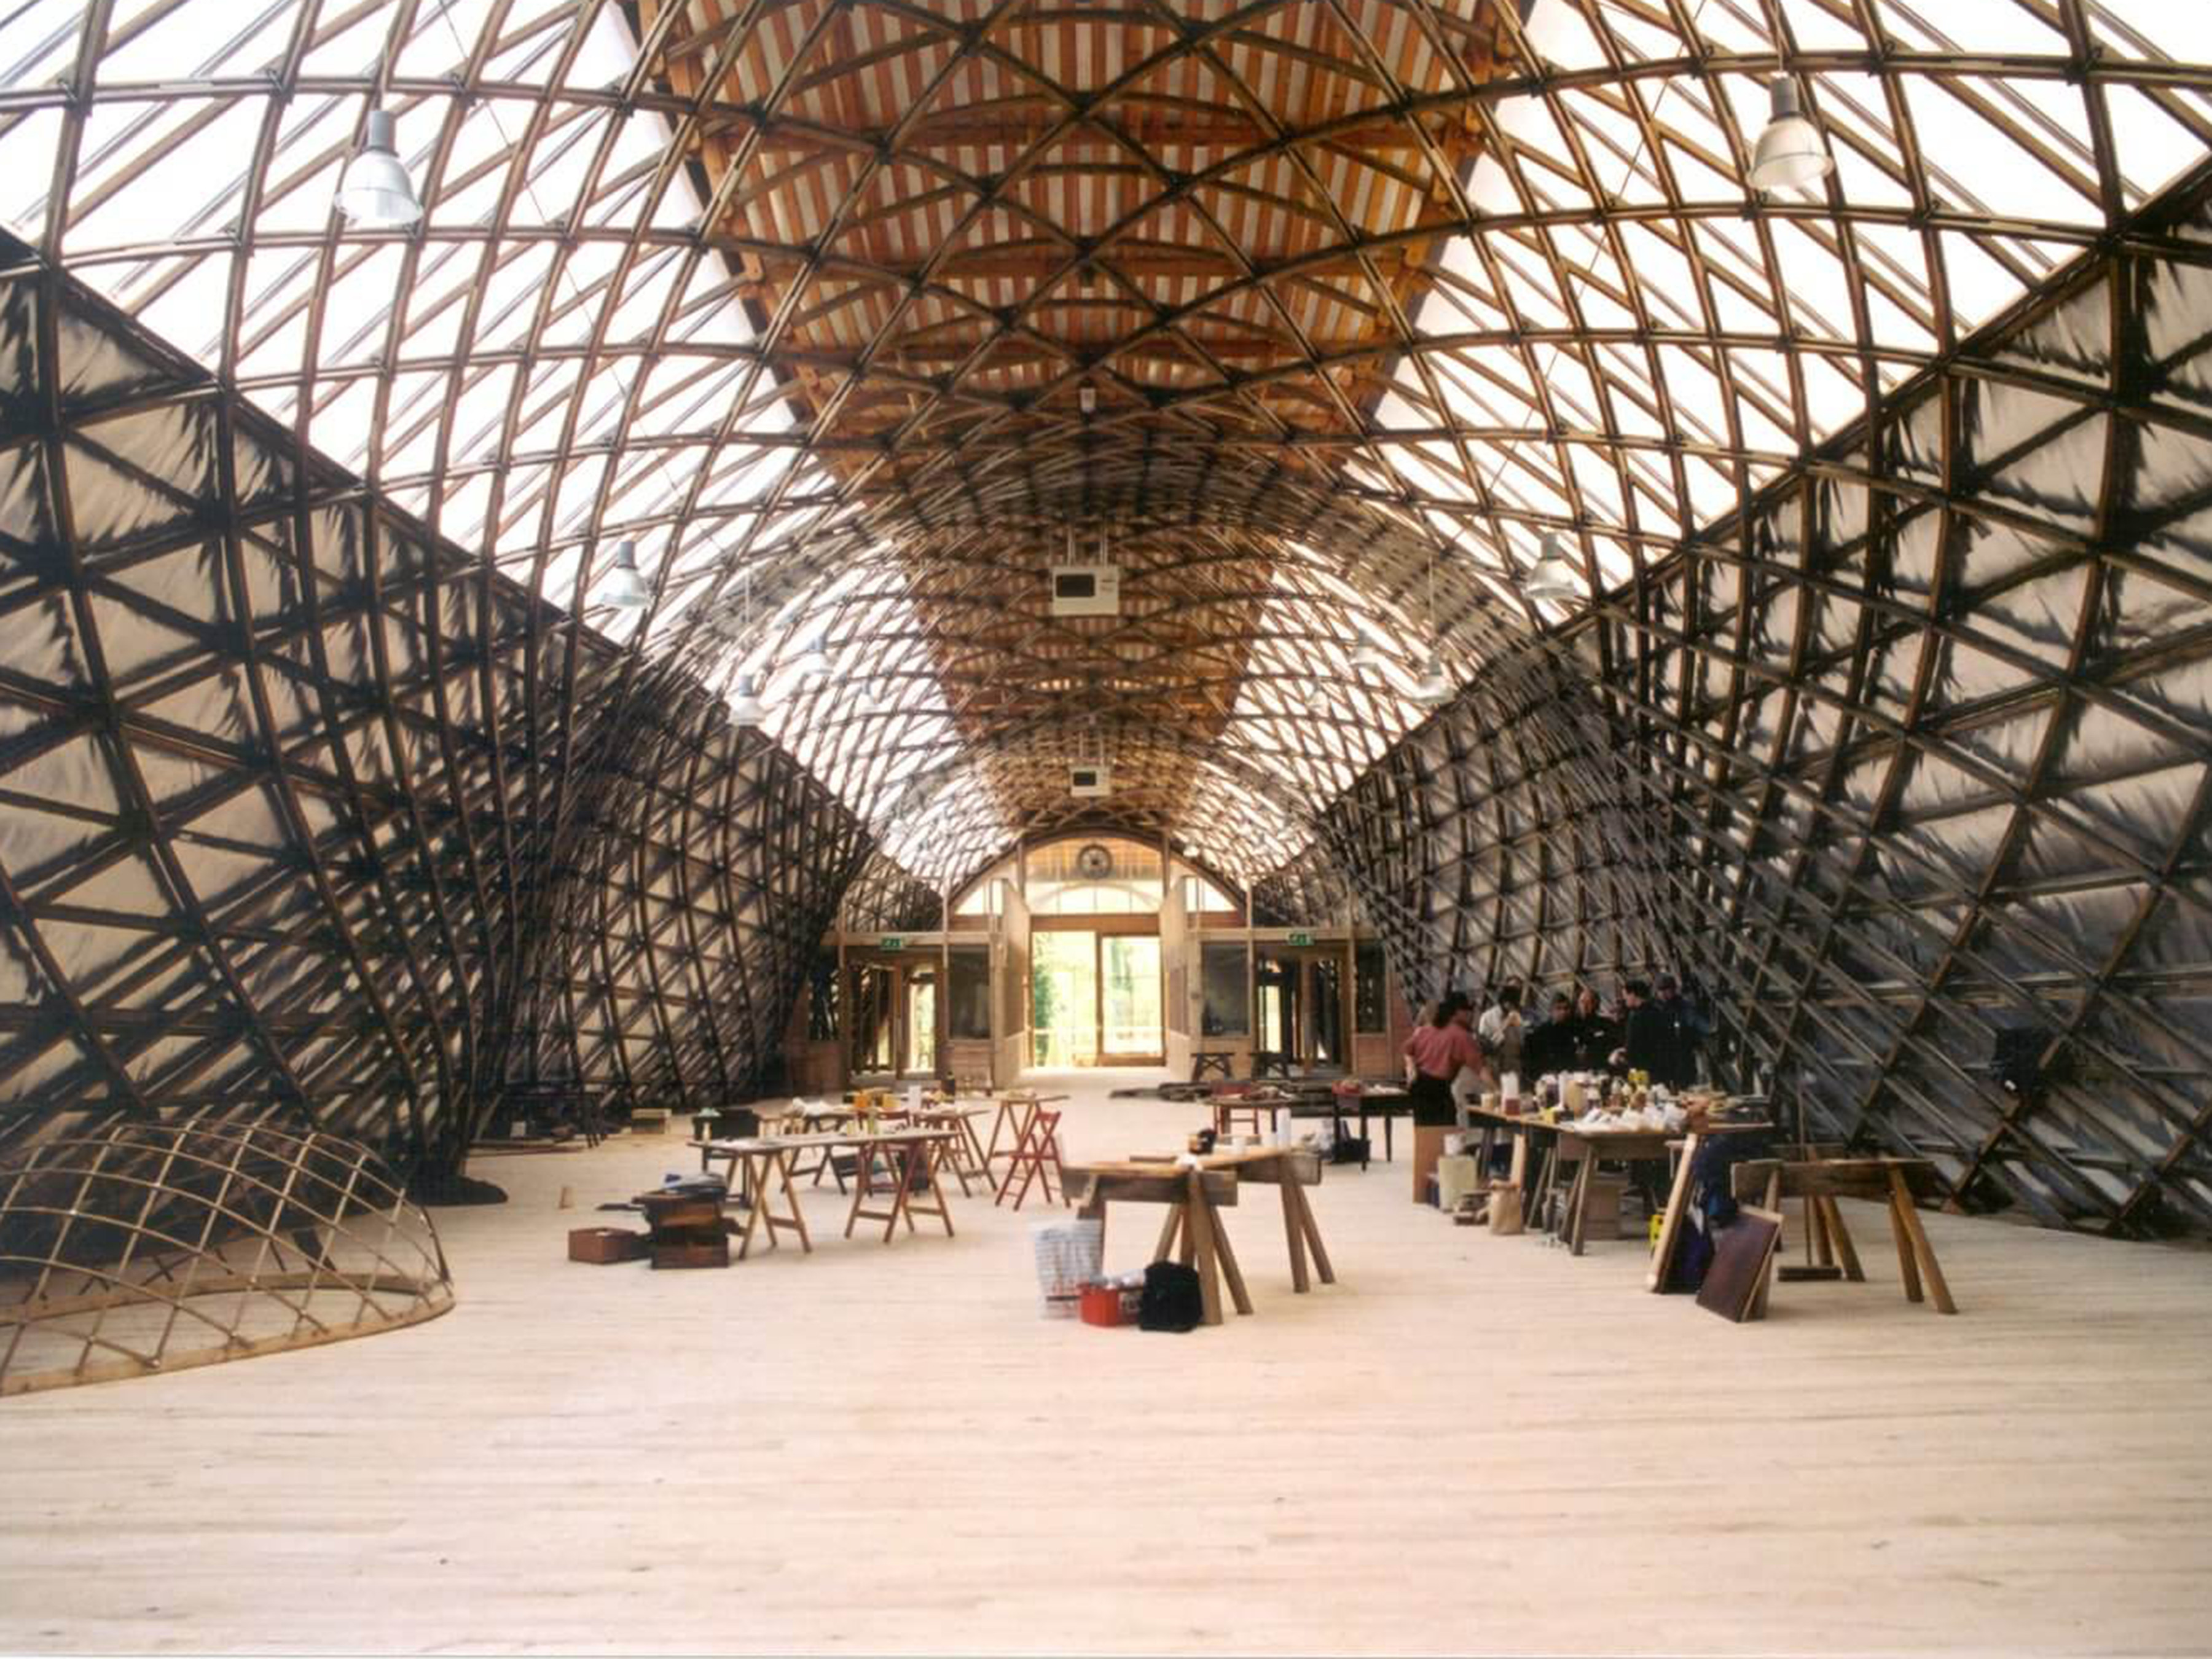
\includegraphics[width=0.48\textwidth]{downland_b.jpg}\label{fig:downland_a}}
		\hspace*{\fill}
		\subfloat[][Exterior view]{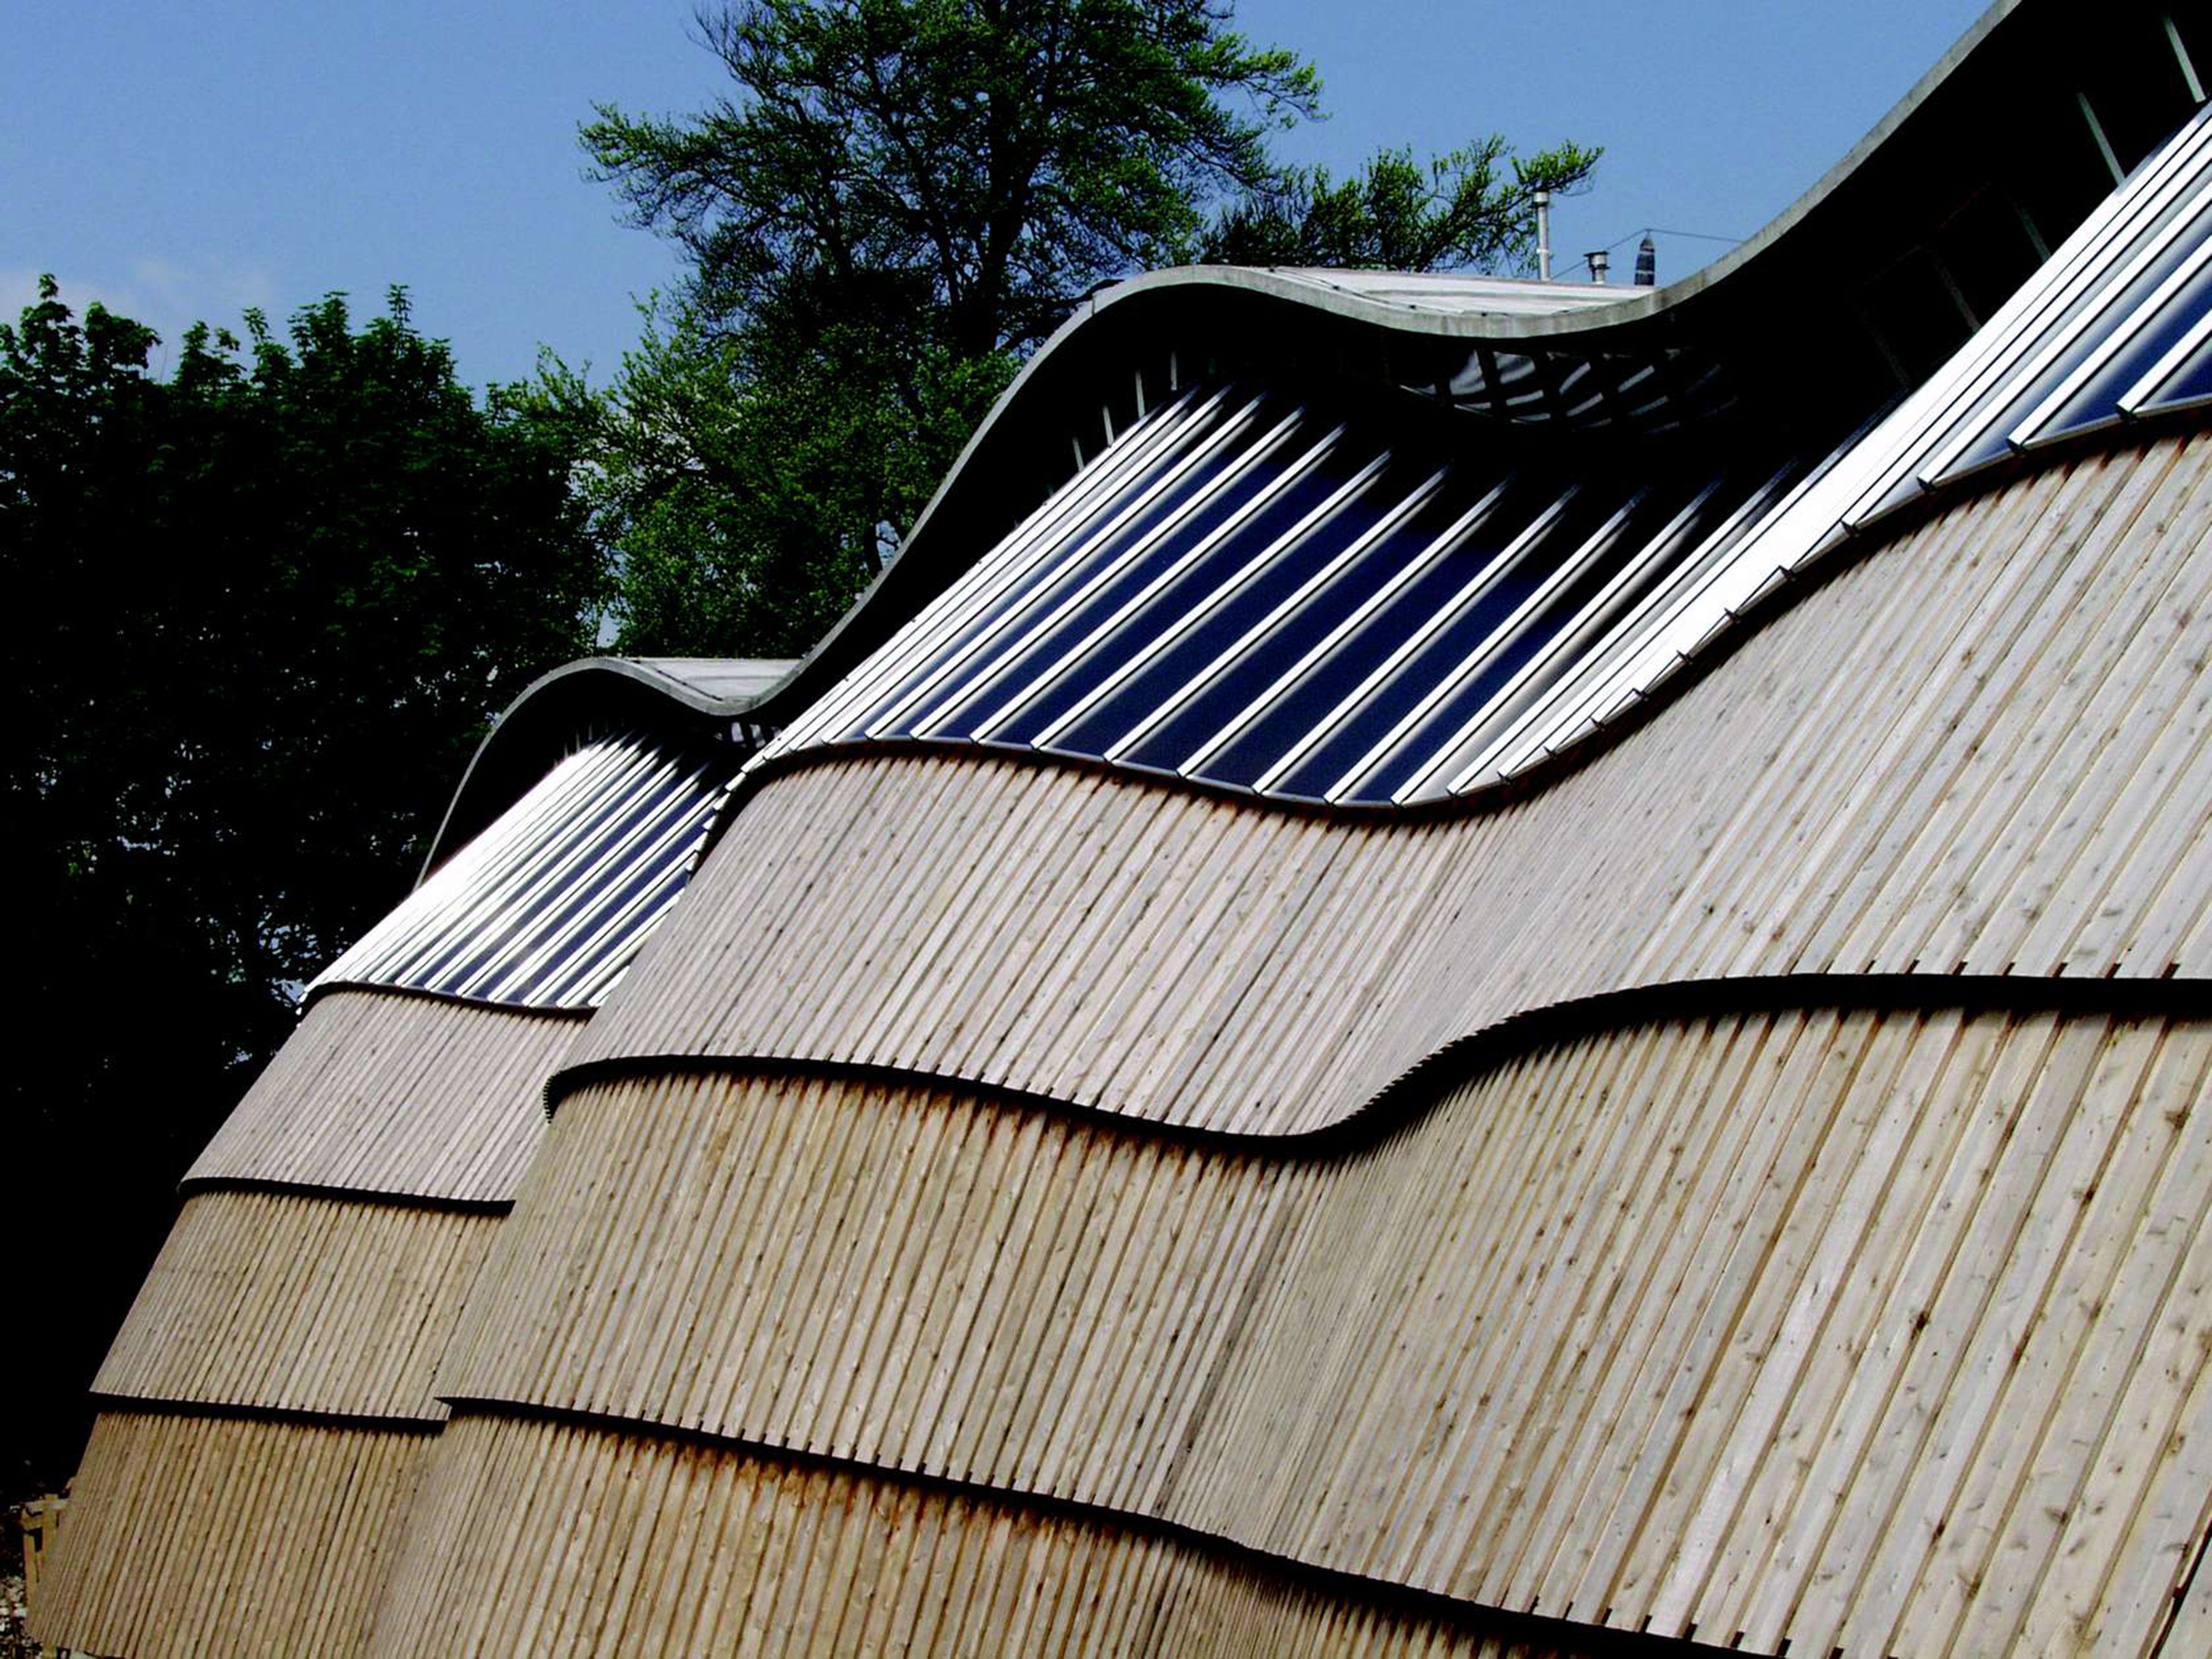
\includegraphics[width=0.48\textwidth]{downland_a.jpg}\label{fig:downland_b}}
		\vspace{10pt}
		\captionof{figure}[Timber gridshell built in 2002 in Downland, England]{Timber gridshell built in 2002 in Downland, England.}
		\label{fig:downland}
%	\end{fullpage}
\end{figure}

The grid pitch is \SI{1.0}{m} except in weaker areas where it is \SI{0.5}{m}. There, the grid is twice denser to achieve the required buckling resistance \cite{Harris2003}. Rib-lath bracing was preferred to steel cable bracing as ribs were deemed to offer a more convenient support for the cladding and to reduce the complexity of the connection. A new connection system was developed to avoid the cost of drilling thousands of slotted holes that would, in addition, reduce the cross-section area, while maintaining the required scissor behaviour for the deformation of the timber lattice.\footnote{This detail was \href{https://patents.google.com/patent/GB2361504A/en?q=\%22A+coupling+and+a+method+of+constructing+grid+shell+buildings+using+such+a+coupling\%22&country=GB}{patented} by the design team and the client.}

The flat lattice was laid out on a scaffold platform. Unlike the Japan Pavilion, the lattice was progressively lowered down into position. This stage took 6 weeks. Once deformed, the shear blocks were introduced in the grid and bracing rib-laths were installed, giving its full strength to the shell. Finally the gridshell was cladded with a mix of polycarbonate plates (to let the light in) and timber boards on top of insulation panels and a rain screen.

It is worthwhile to mention that for the first time the form was not found by inverting some sort of hanging chain model that would produce a pure funicular shape where only compression occurred. Instead, the shape was the result of a numerical computation that took into account the bending behaviour of the laths.\footnote{This software was developed under the supervision of Chris Williams of the university of Bath.} \citet{Harris2003} argued that computer models enabled some interactivity in the form-finding process that would not be possible with physical models, leading to a better synergy between architectural and structural requirements. They also argued that physical models contributed invaluably to the development of a creative and efficient design throughout the project.

\subsubsection{Lothian Gridshell, Pishwanton, Scotland, 2002}
This project deserves some attention because the developed approach was completely different from the projects exposed until now~: \blockcquote[]{Lowenstein2002}{Previous projects have portrayed the method as a highly technical use of a low-tech resources. This, however, needs not be the case as we see with this project \belp{}}. The structure was the result of \blockcquote[]{bdonline2002}{\belp{} an unusual collaboration between sole practitioner Christopher Day, engineer David Tasker, a crowd of local volunteers and (more unusually) the philosophies of Rudolf Steiner and Johann Wolfgang Goethe}.\footnote{From the online paper \textquote{The other gridshell} : \url{http://www.bdonline.co.uk/the-other-gridshell/1020435.article}}

The single-layer gridshell was made out of local larch. Once erected by hands, the dome-like shape covered about \SI{80}{m^2} and spanned 10 meters. The grid was braced with timber boards (see \cref{fig:pishwanton_a}) and covered with a planted turf roof (see \cref{fig:pishwanton_b}). Some calculations were made but in the end, it had to carry load testing to prove its safety and gain its regulation approval.\footnote{\blockcquote[]{bdonline2002}{There were a lot of calculations but no computer-generated models to show they all added up. In fact, the form was previously established with scale models. When it came to gaining Building Regulations approval, the team needed to prove that the building would be strong enough. So Tasker arranged for the unfinished structure to be loaded with about 18 tonnes of sand from a local quarry – equivalent to the maximum predicted snow load, plus a safety factor.}}

\subsubsection{Woodland Centre, Filmwell, England, 2003}
The gridshell of the Woodland Centre was built 7 years after the project had started (see \cref{fig:flimwell_a}).\footnote{More to be found at : \href{http://www.fourthdoor.org/annular/?page_id=441}{Growing and making Flimwell’s chestnut gridshell}.} The building was designed by architect Feilden Clegg and engineers from Atelier One. It was part of a larger research and development project that aimed at developing chestnut -- a low grad wood -- as a construction material.\footnote{This projet was conducted by the \href{http://www.bre.co.uk/}{Building Research Establishment}.}

The building, still existing, is composed of 5 barrel vaults spanning 12 meters and about 5 meters wide (see \cref{fig:flimwell_b}). It covers about \SI{300}{m^2} \cite{Lowenstein2004}. Each vault module is a transportable unit composed of two curved arches. A single layer gridshell was then applied to this primary frame and braced with chestnut panels. The grid was made of laths with~\SI{75}{mm} x \SI{25}{mm} rectangular cross-section, assembled with simple bolts. On top of that, insulation materials and a membrane as rainscreen \cite{FourthDoor2003}.

\begin{figure}[p]
     	\centering
%	\begin{fullpage}
		\subfloat[][Interior view]{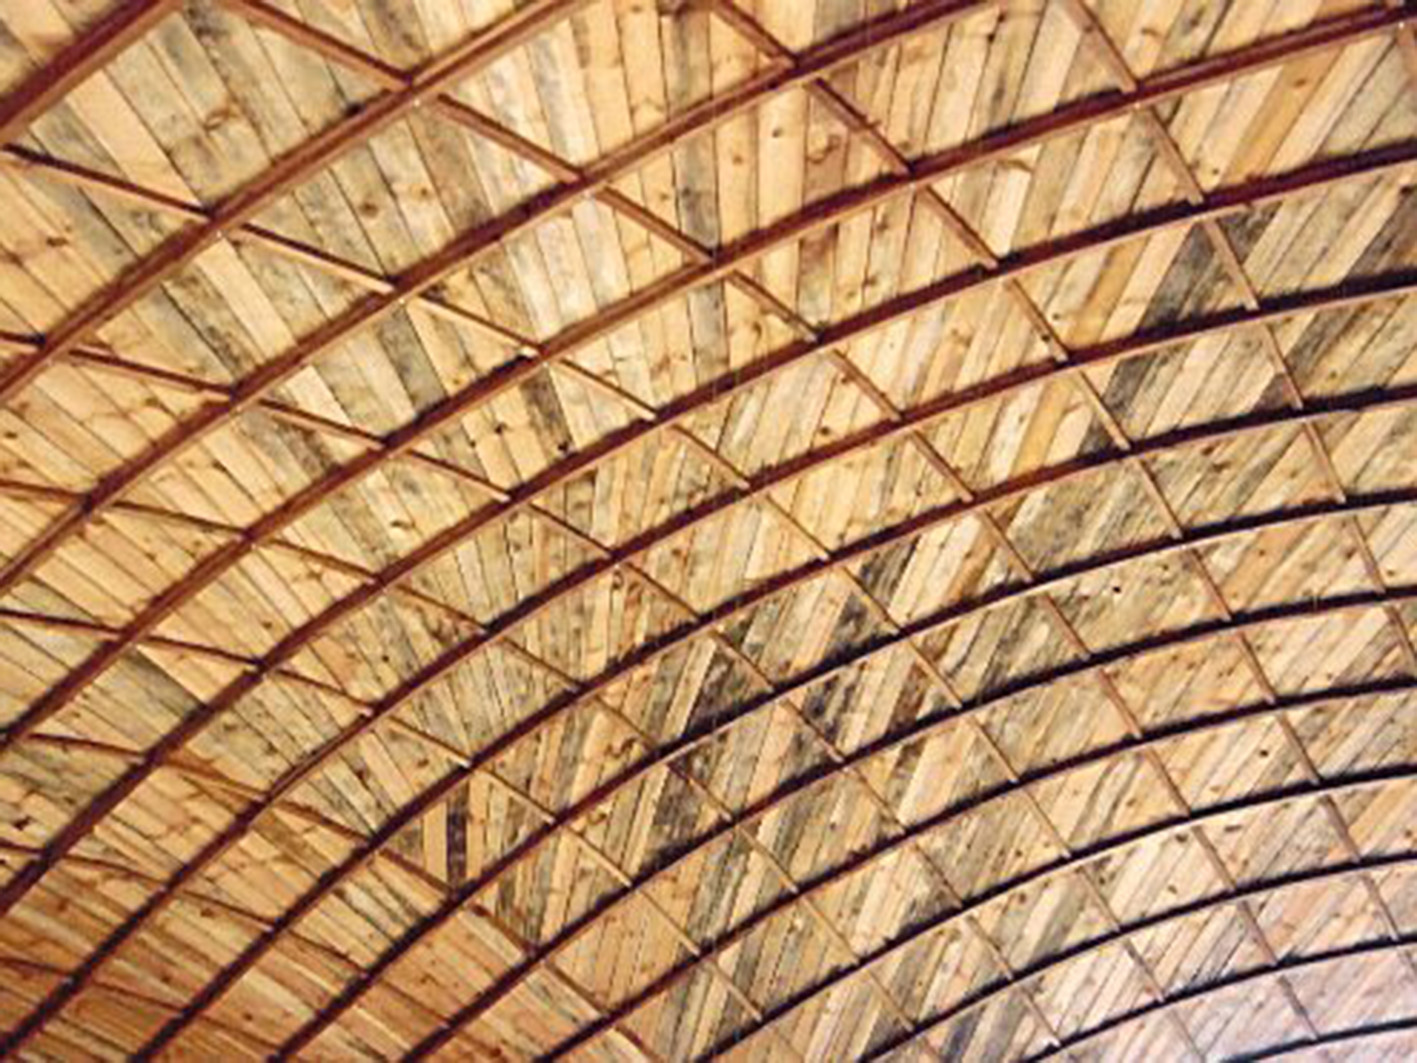
\includegraphics[width=0.48\textwidth]{pishwanton_int.jpg}\label{fig:pishwanton_a}}
		\hspace*{\fill}
		\subfloat[][Exterior view]{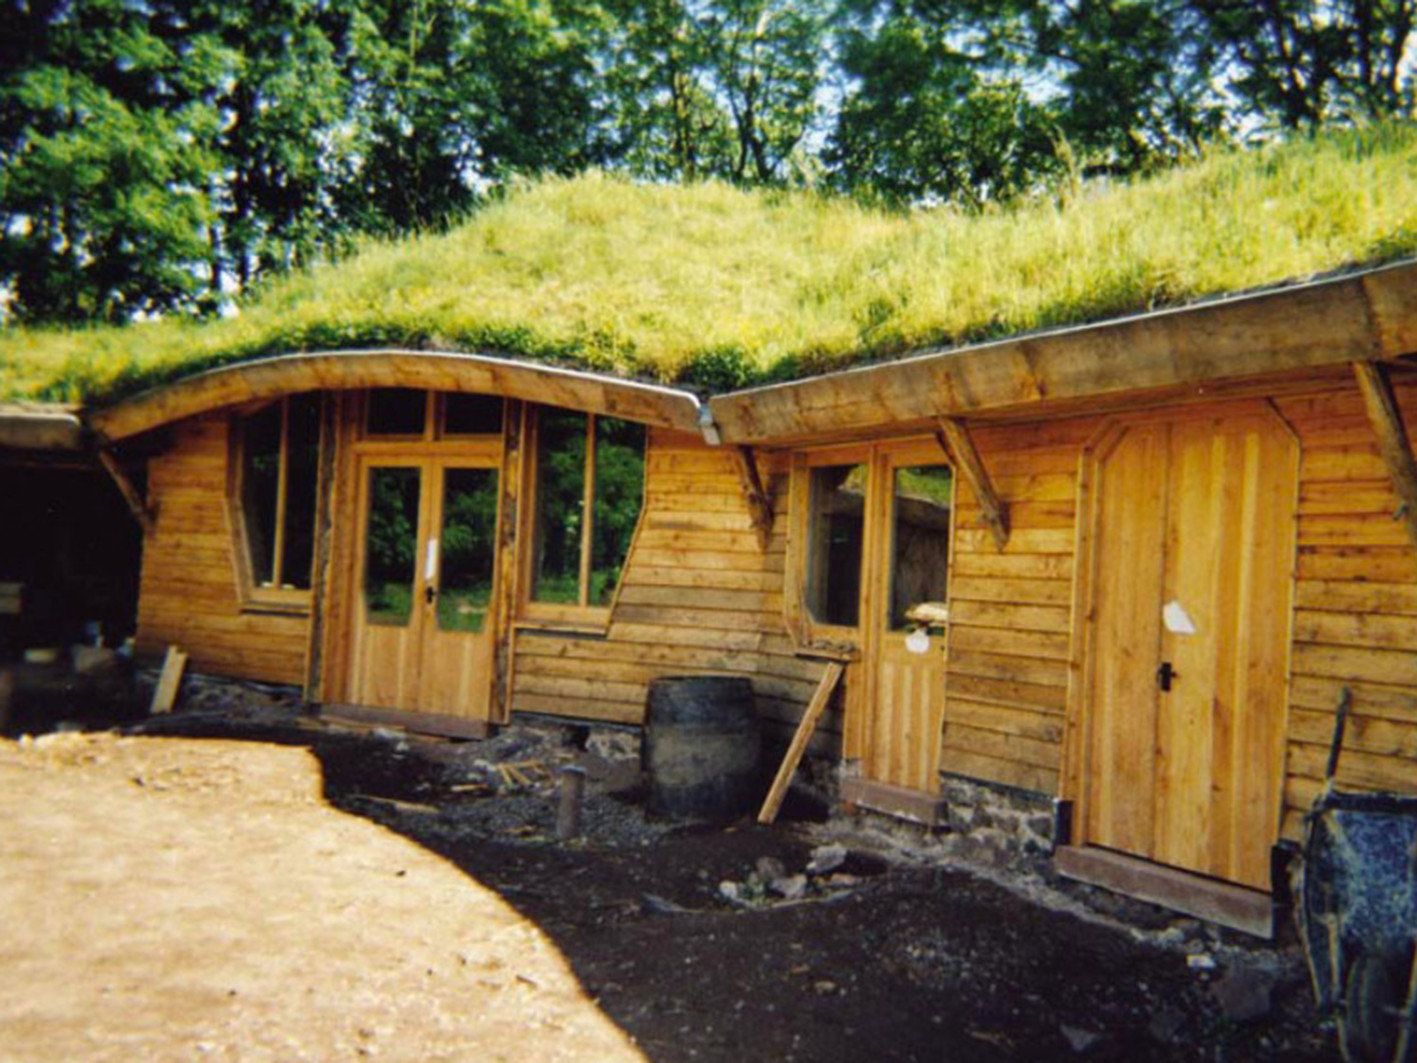
\includegraphics[width=0.48\textwidth]{pishwanton_ext.jpg}\label{fig:pishwanton_b}}
		\vspace{10pt}
		\captionof{figure}[Timber gridshell built in 2002 in Pishwanton, England]{Timber gridshell built in 2002 in Pishwanton, England.}
		\label{fig:pishwanton}
		%
		\vspace{0.5cm}
		%
		\subfloat[][Interior view]{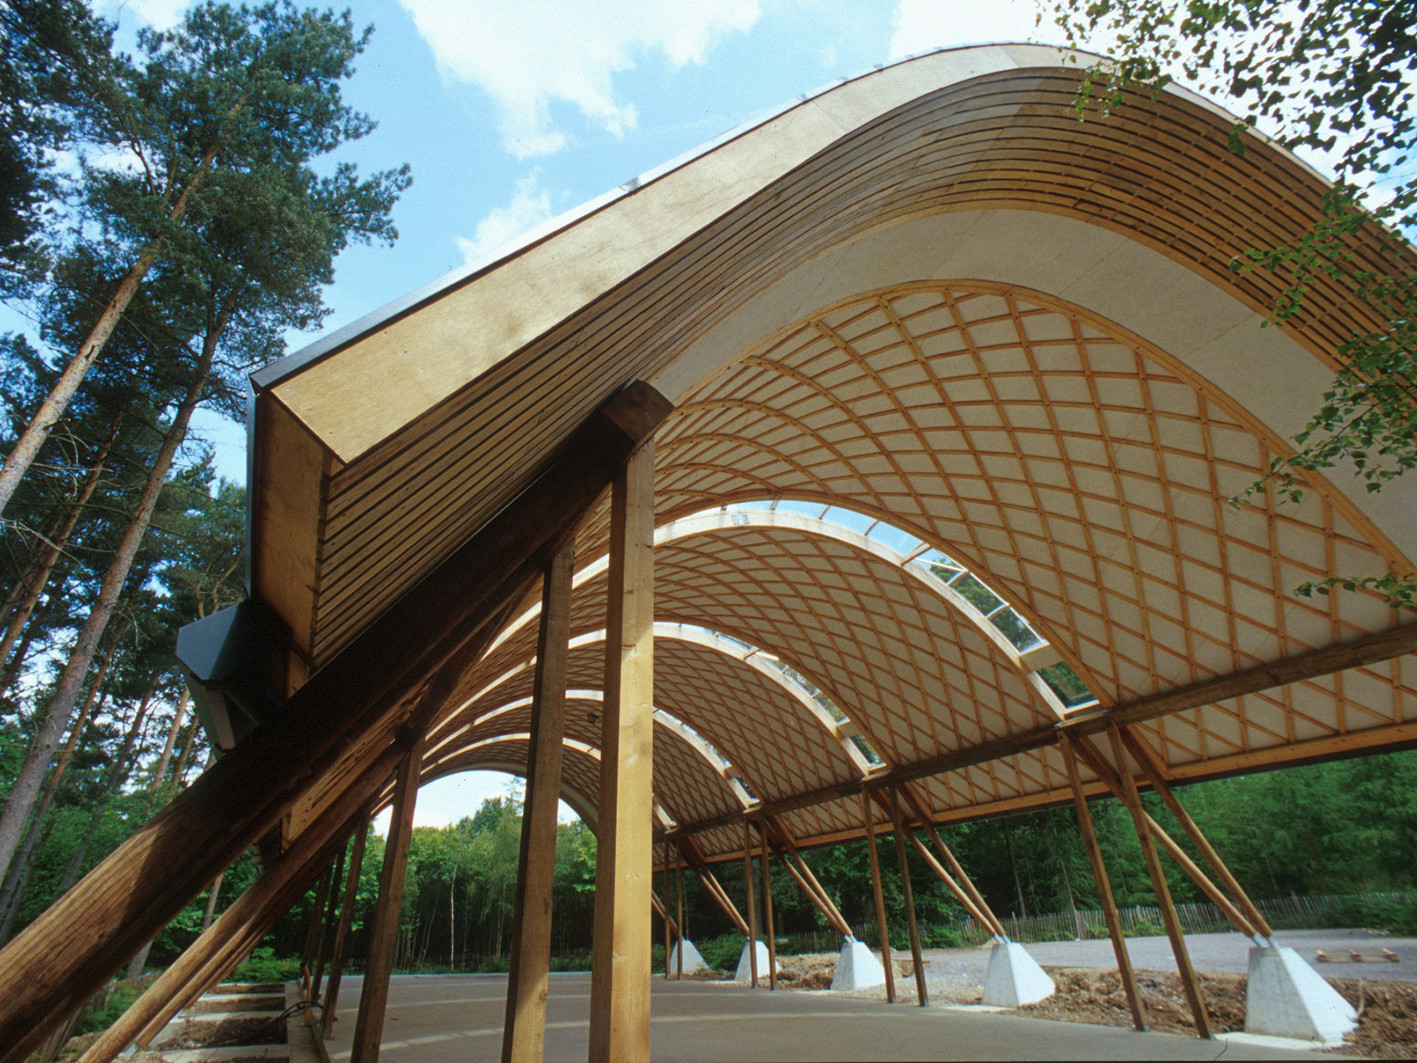
\includegraphics[width=0.48\textwidth]{flimwell_int.jpg}\label{fig:flimwell_a}}
		\hspace*{\fill}
		\subfloat[][Exterior view]{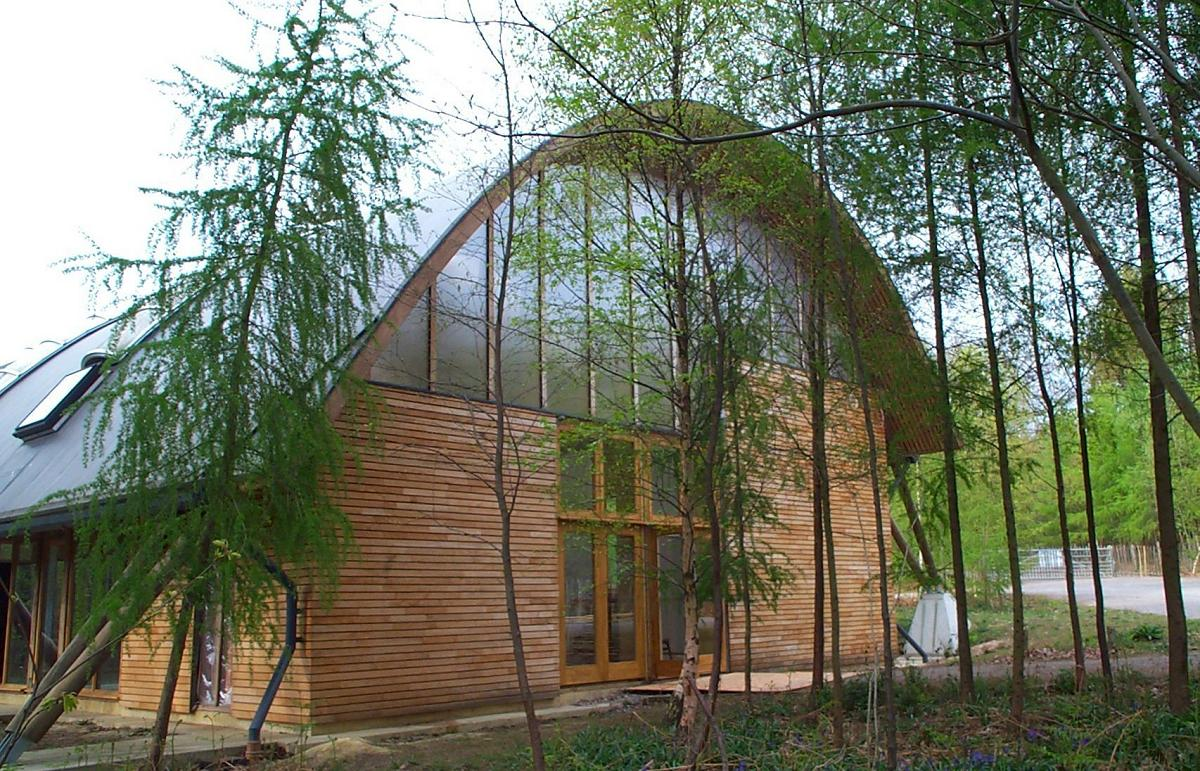
\includegraphics[width=0.48\textwidth]{flimwell_ext.jpg}\label{fig:flimwell_b}}
		\vspace{10pt}
		\captionof{figure}[Timber gridshell built in 2003 in Filmwell, England]{Timber gridshell built in 2003 in Filmwell, England.}
		\label{fig:flimwell}
		%
		\vspace{0.5cm}
		%
		\subfloat[][Interior view]{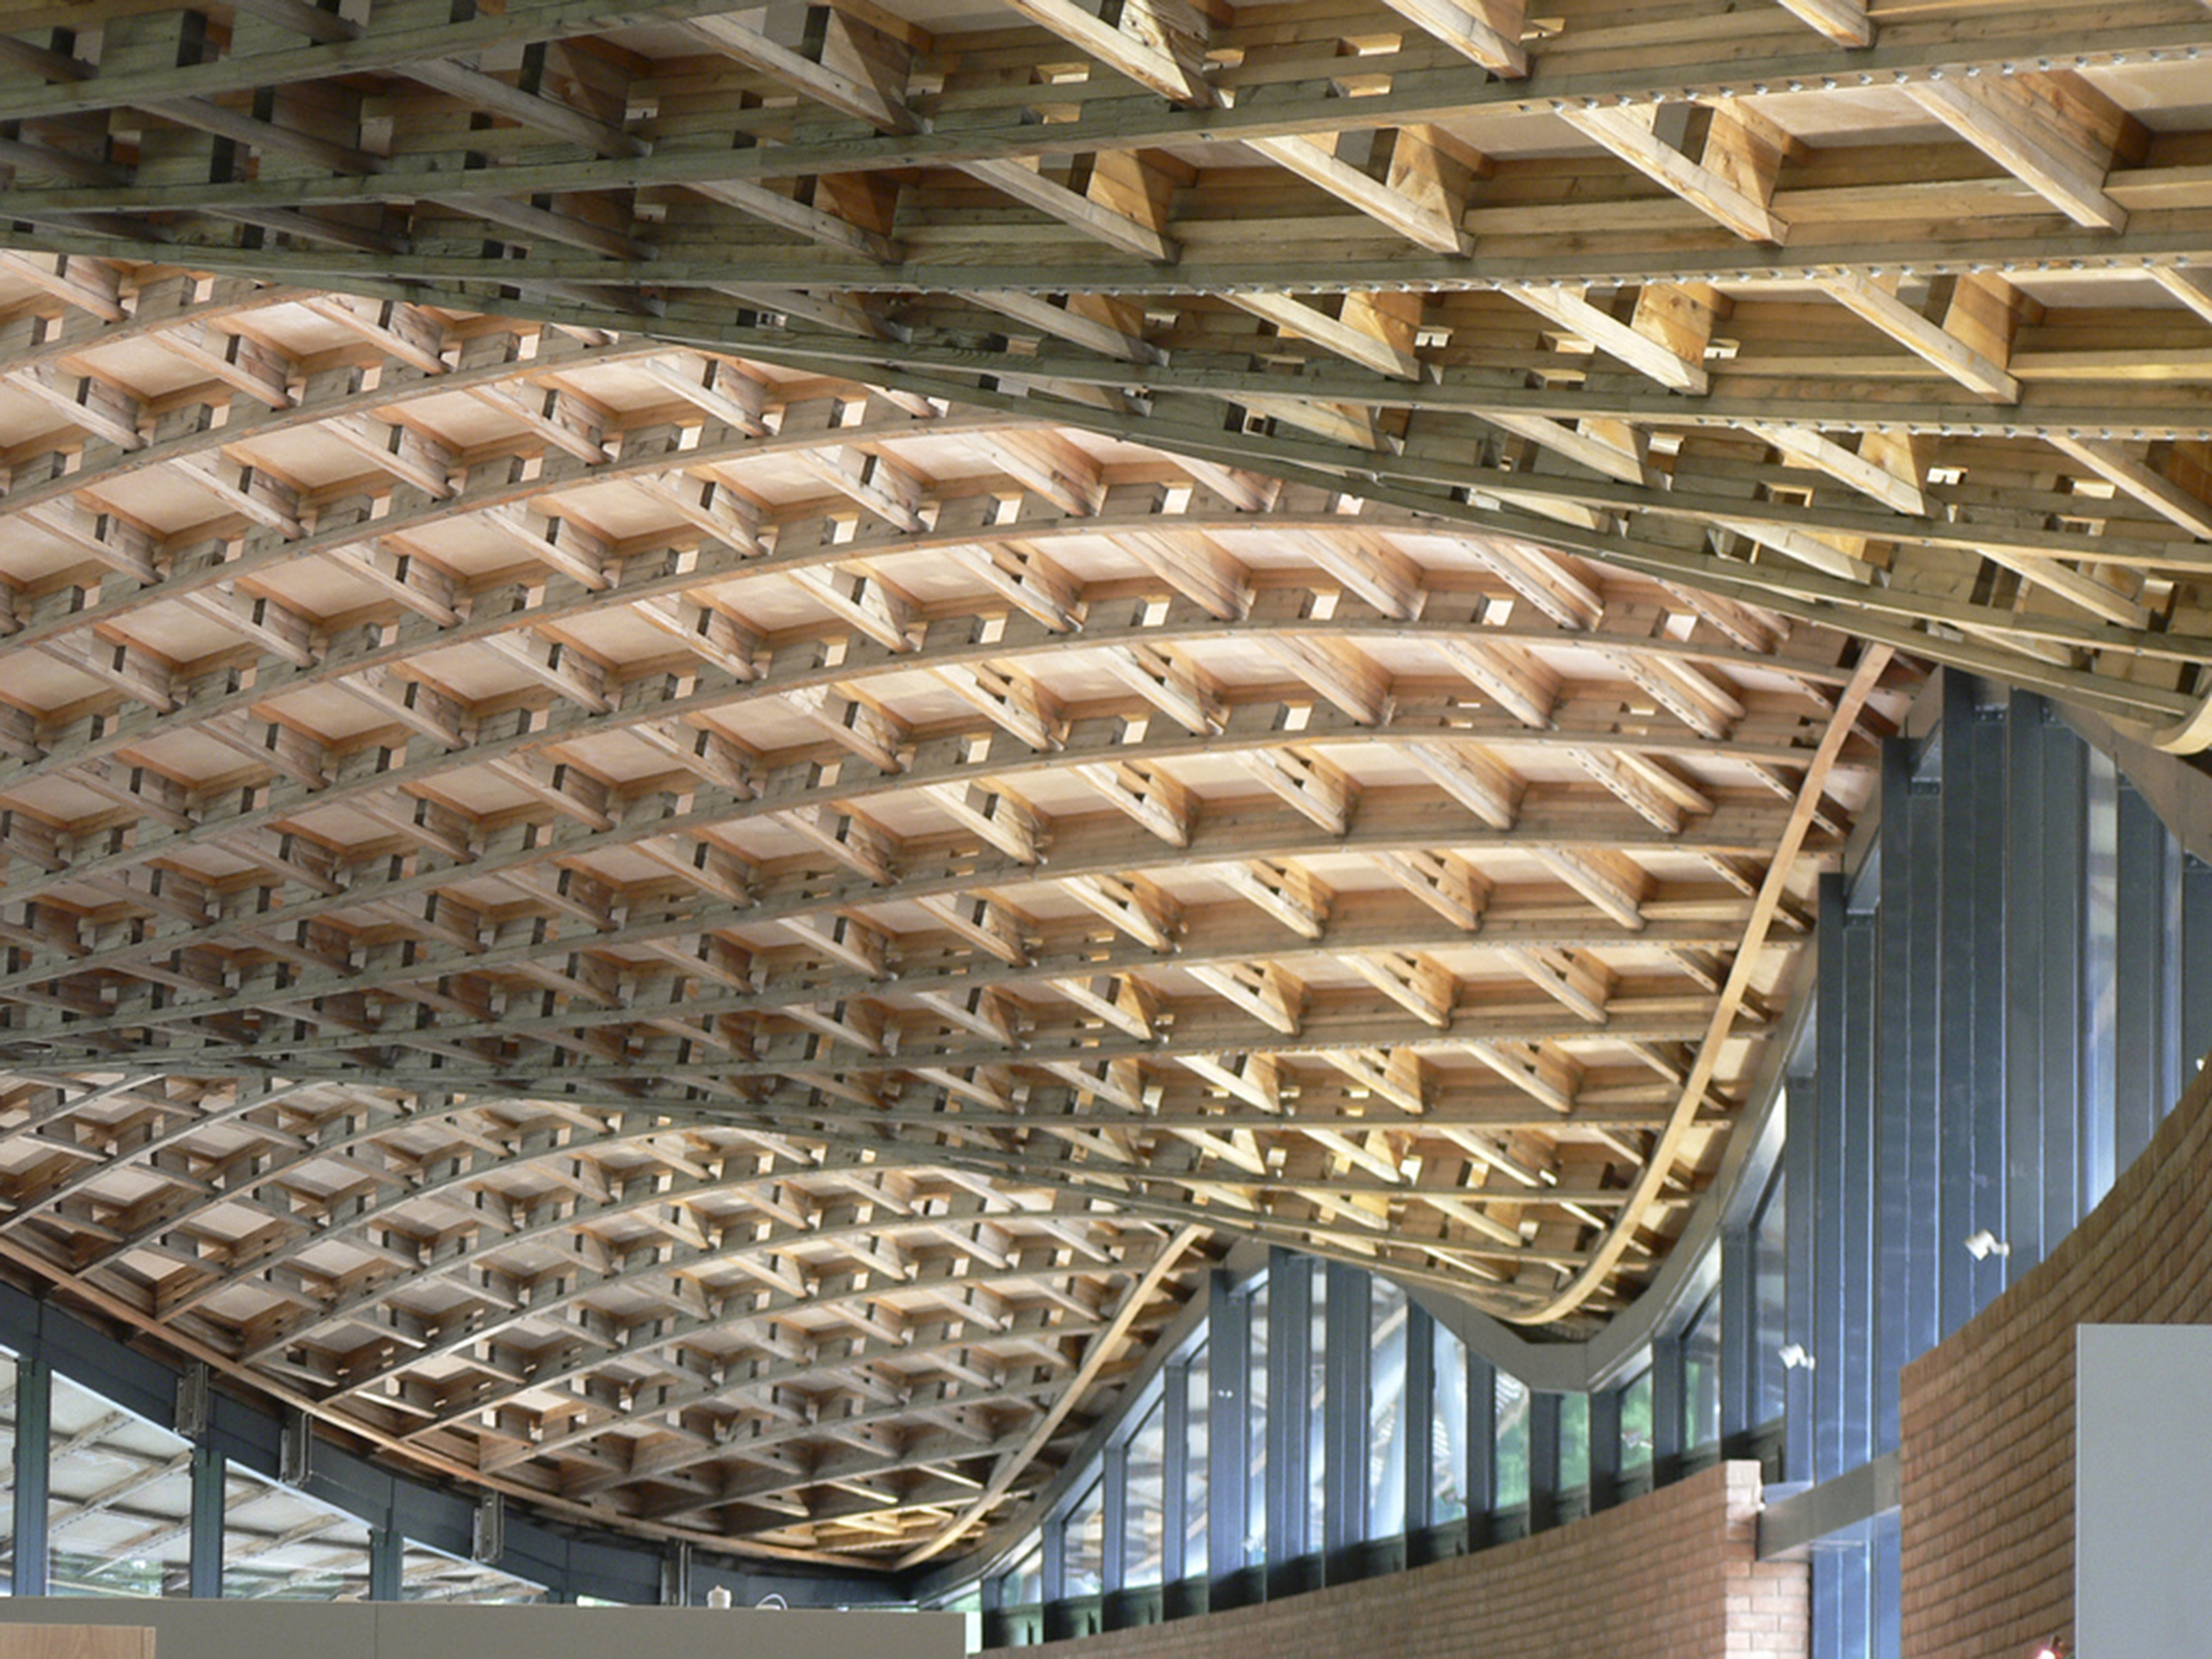
\includegraphics[width=0.48\textwidth]{savill_b.jpg}\label{fig:savill_a}}
		\hspace*{\fill}
		\subfloat[][Exterior view]{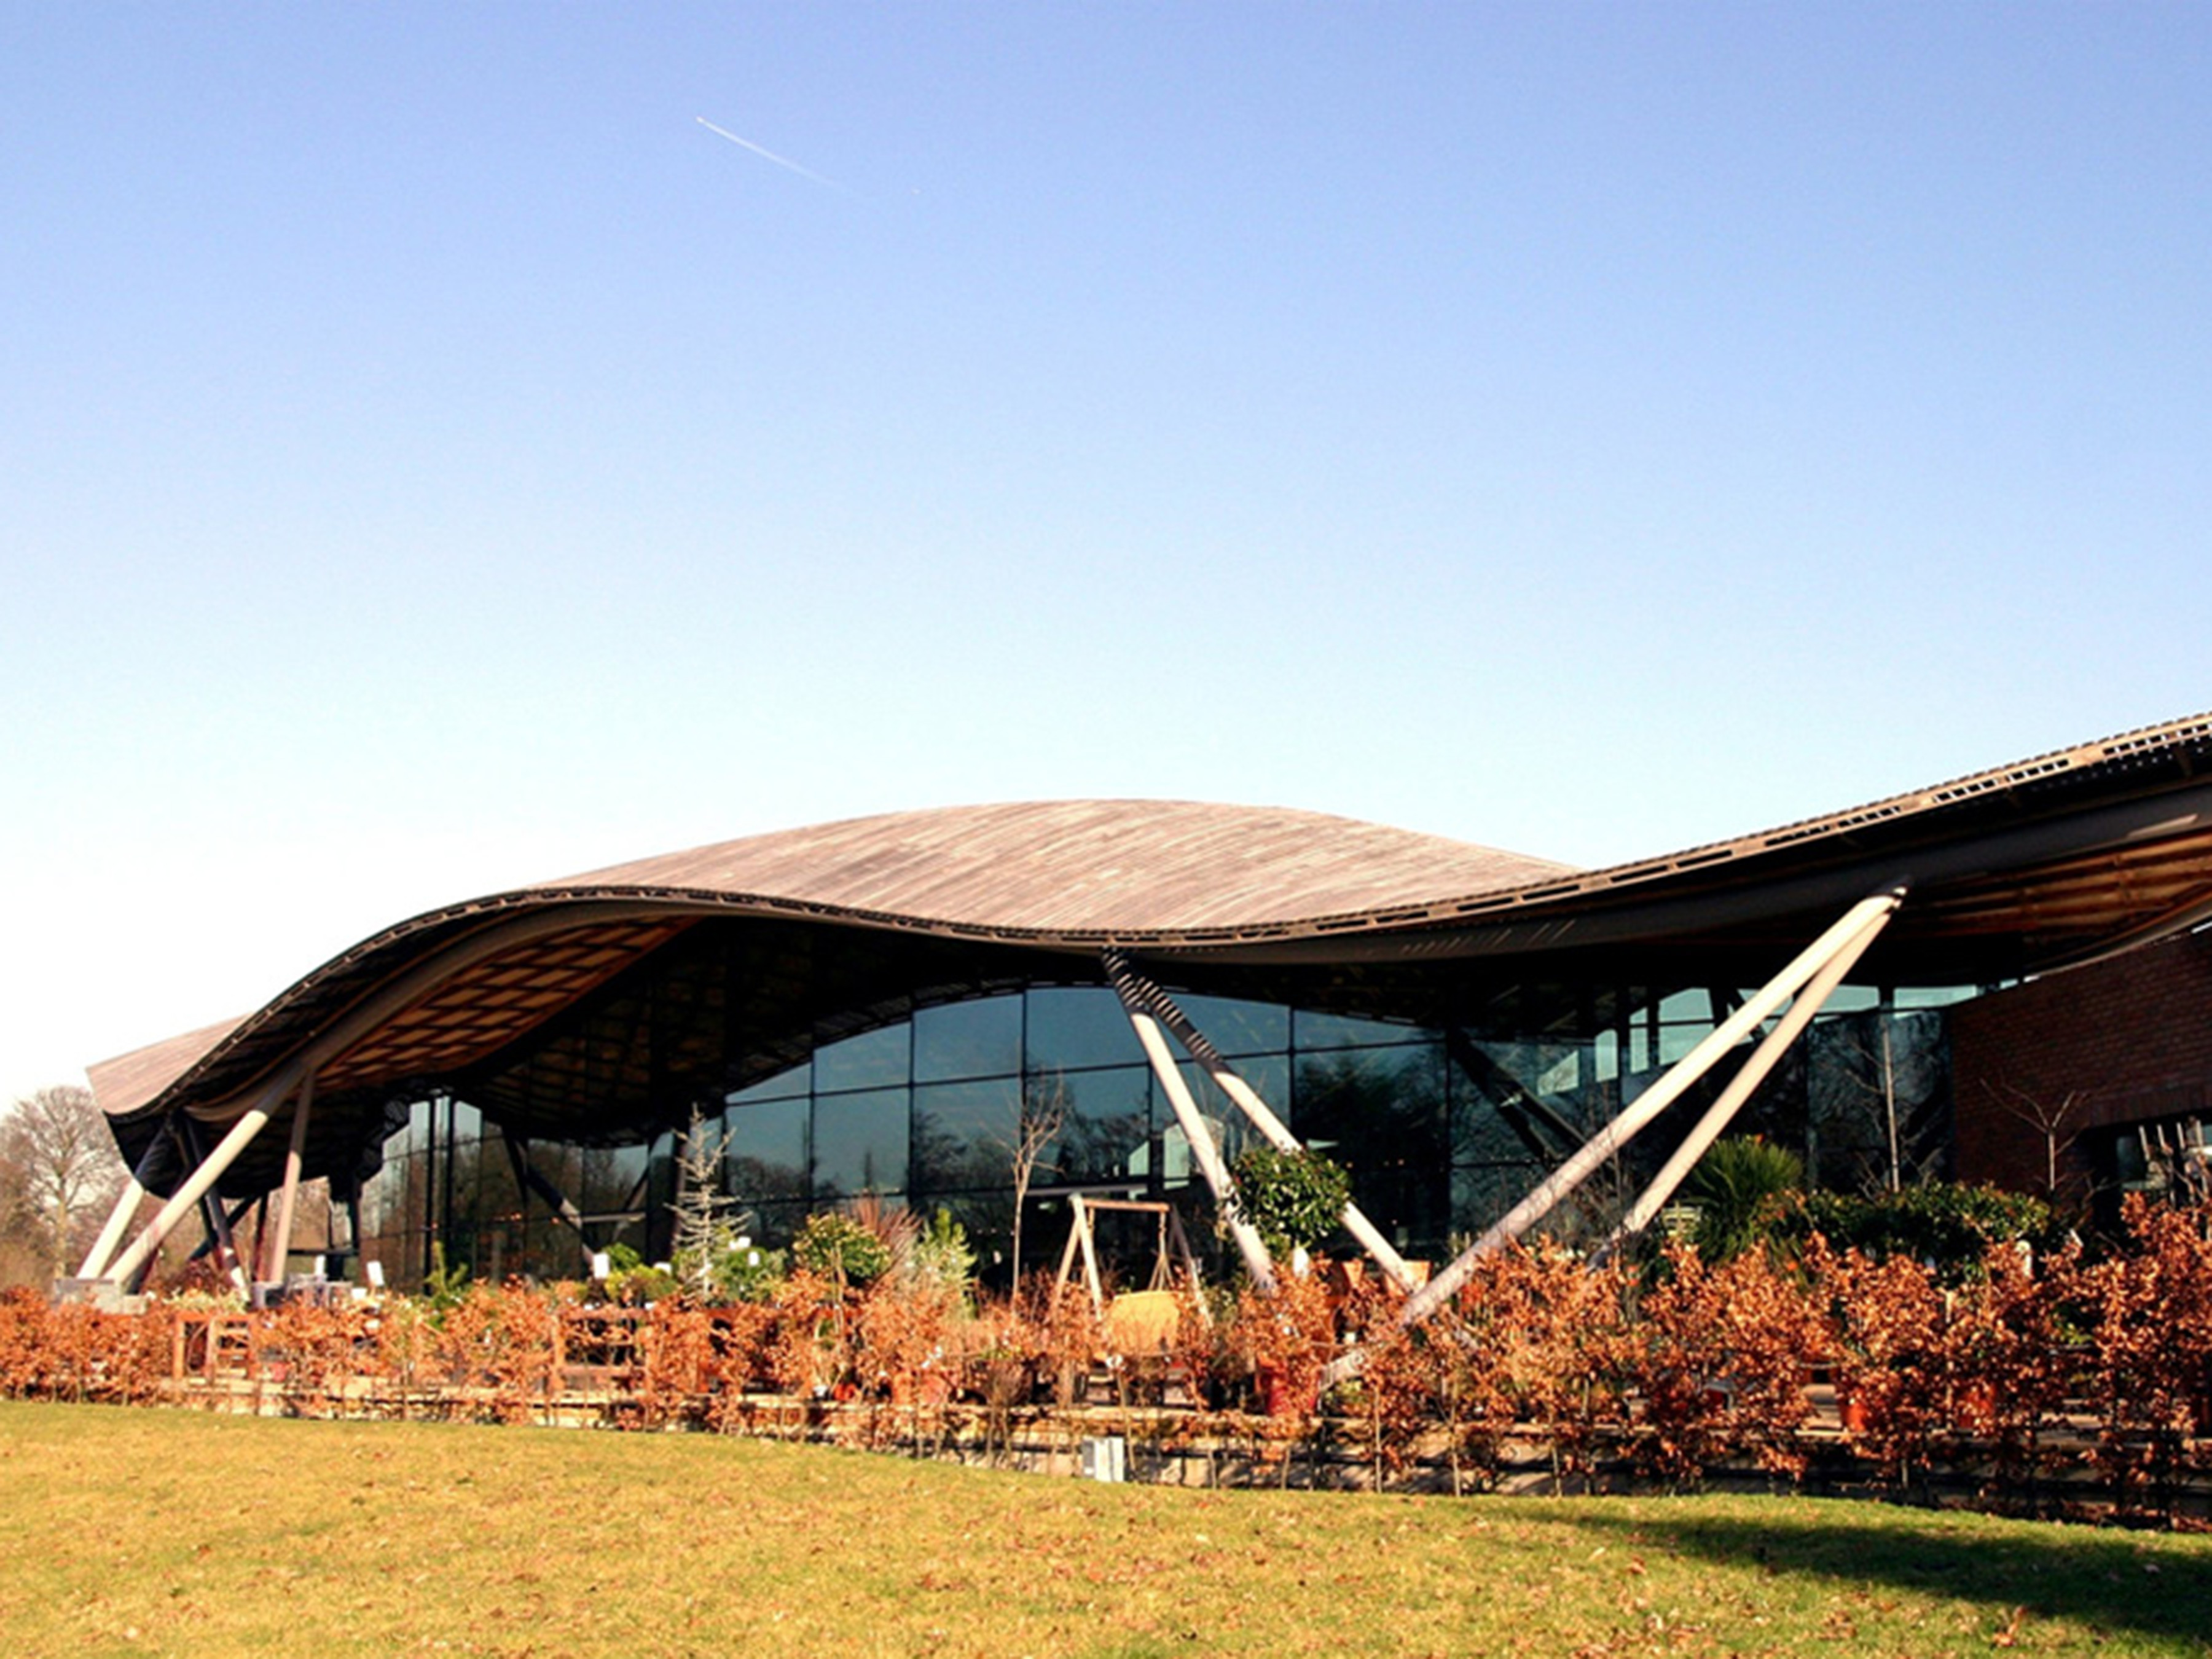
\includegraphics[width=0.48\textwidth]{savill_a.jpg}\label{fig:savill_b}}
		\vspace{10pt}
		\captionof{figure}[Timber gridshell built in 2006 in Savill, England]{Timber gridshell built in 2006 in Savill, England.}
		\label{fig:savill}
%	\end{fullpage}
\end{figure}

\subsubsection{Savill Garden, Englefield Green, England, 2006}

This project saw the light of day thanks to the reputation of the gridshell built in Downland. Again, Buro Happold did the structural design while Green Oak Carpentry realised it. But this time, the architect was Glenn Howells.

The \emph{Savill} gridshell is 90 meters long and 25 meters wide. It covers an area of about \SI{2000}{m^2}, and is therefore almost three times larger than the gridshell in Downland. Once again, the corrugated shape was defined by a parametric equation ($z = f(x,y)$) to enable interactivity between architects and engineers during the form-finding process (see \cref{fig:savill_b}). Chris Williams was responsible for this job \cite{Harris2008}.

In Savill, the forming strategy was quite different than those employed in Mannheim, Hannover or Downland \cite{Harris2008}. Firstly, a single layer gridshell -- constituted by the bottom two laths jointed with simple bolts -- was deformed into the target shape. Secondly, the shear blocks were screwed on these laths. Thirdly, the upper two laths were positioned and screwed on top of the shear blocks to re-form a double-layer gridshell. Finally, the grid was braced with two alternate layers of plywood boards, \SI{12}{mm} thick each. Bracing the grid with continuous panels instead of cables or diagonal members was a major architectural choice (see \cref{fig:savill_a}). Moreover, it gave a well-defined surface for the cladding composed of \SI{160}{mm} of insulation, covered by a waterproof aluminium layer made with standing-seam profiles supporting the oak boards \cite{Trada2006}.

Another consequence of this forming process was the drastic simplification of the connexion. The system developed for Downland was of no utility in that case and only simple bolts and screws were required. In this project, the pitch of this grid is \SI{1.0}{m}. The \SI{20}{kms} of laths are made from larch and have a \SI{80}{mm} x \SI{50}{mm} rectangular cross-section. They are spaced from \SI{100}{mm} to \SI{150}{mm} by the shear blocks.

Of course, the steel perimeter is a major component of the project but is not in the scope of this thesis. For further details the reader is invited to refer to \citet{Harris2008} and \citet{Trada2006}.

\subsubsection{Chiddingstone Castle Orangery, Kent, England, 2007}
The gridshell covering the orangery of Chiddingstone Castle is a very small one. Built in 2007, it is 12 meters long, 5 meters wide and covers about \SI{50}{m^2} (see \cref{fig:kent_b}). The structural system is derived from the one employed in Downland and is, once again, developed by Buro Happold and the Green Oak Carpentry. But this time the architect is Peter Hulbert.

However this project embed some interesting innovations. Indeed, this time the gridshell is braced with a bidirectional cable network. Twin cables are employed to facilitate clamping on the node connection, which has been adapted from the previous version developed in Downland. This connection is now equipped with an additional threaded hole which can receive the clamping supports for the glazing (see \cref{fig:kent_a}). The timber shell is then glazed with triangular panels. Note that the quadrangles of the mesh are not planar any more in the deformed configuration and therefore triangulation of the (flat) glass panels is mandatory.

\begin{figure}[t]
     	\centering
%	\begin{fullpage}
		\subfloat[][Glazing support]{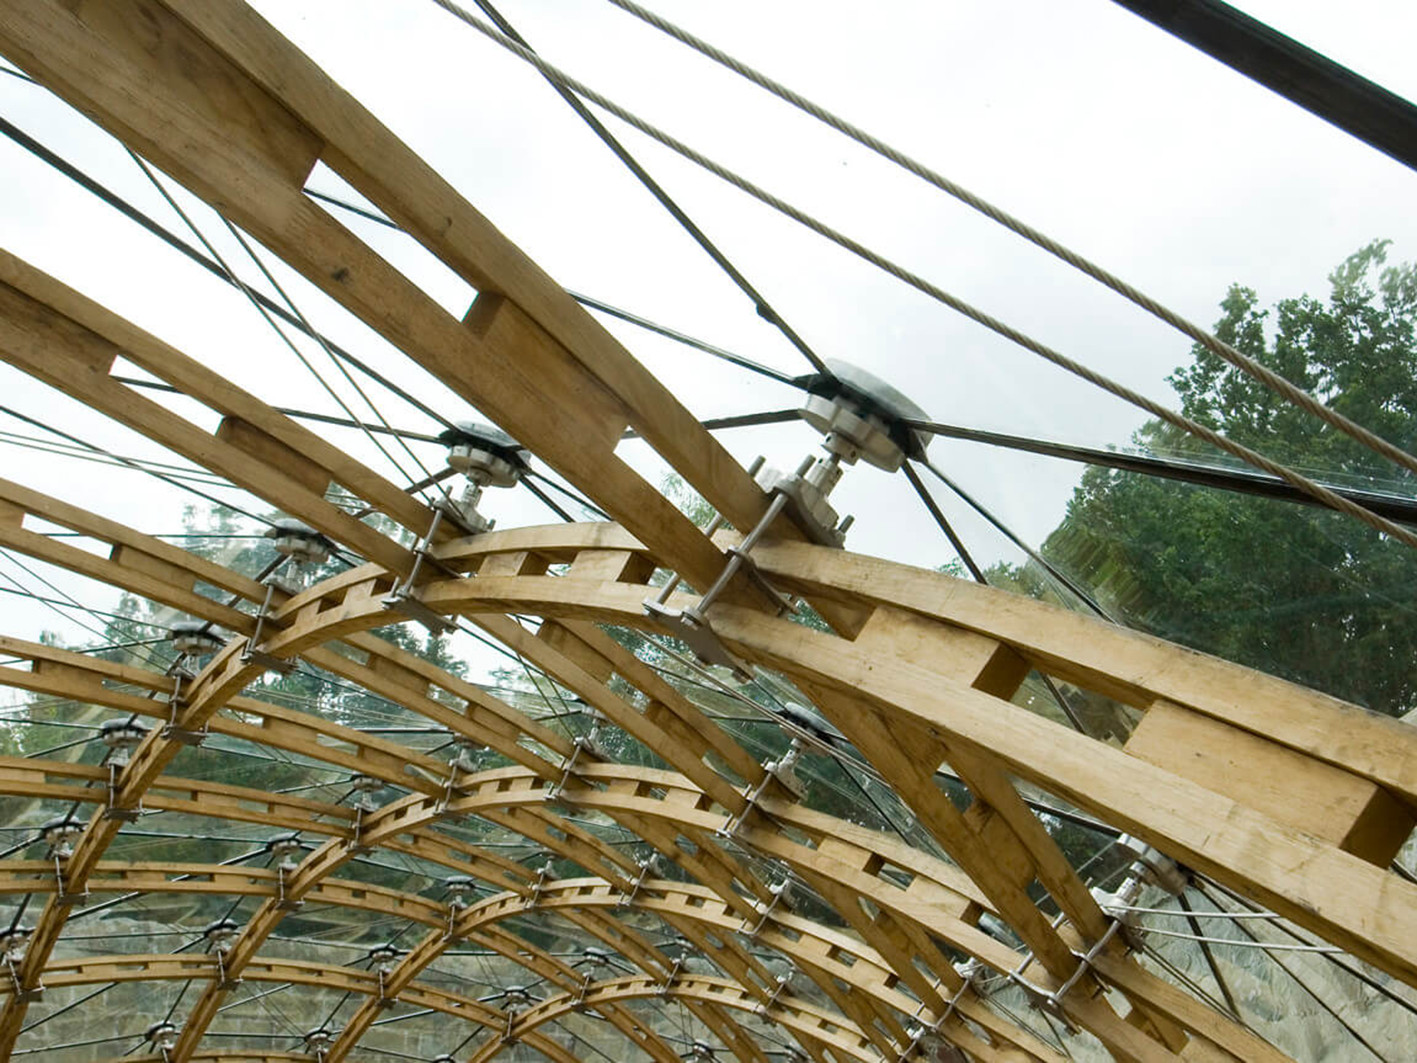
\includegraphics[width=0.48\textwidth]{kent_grid.jpg}\label{fig:kent_a}}
		\hspace*{\fill}
		\subfloat[][Exterior view]{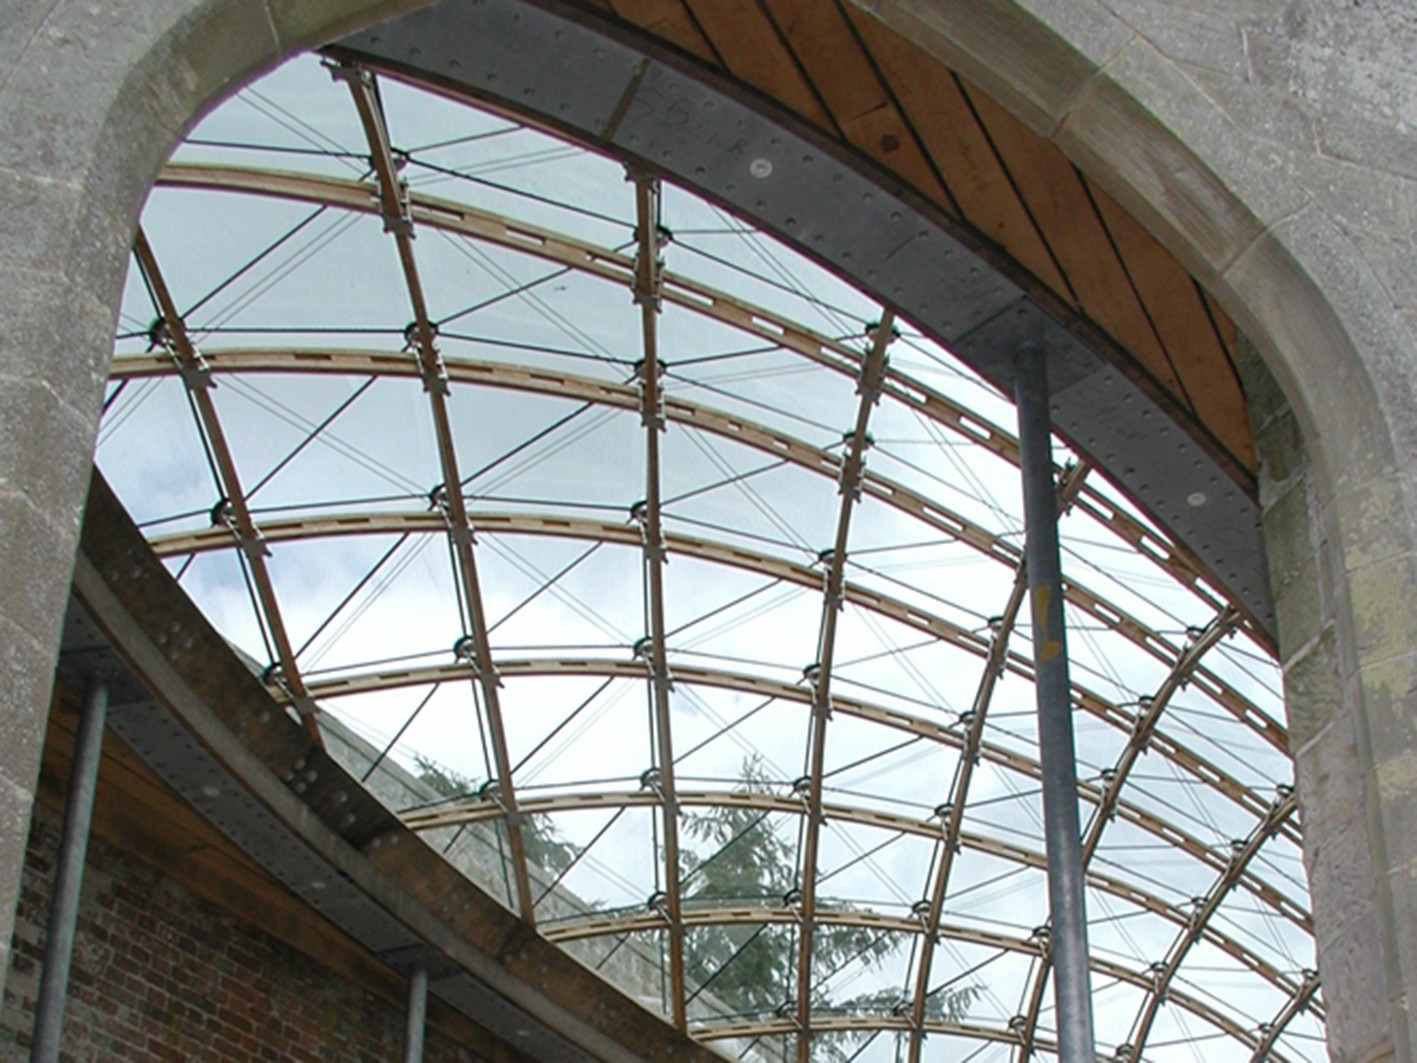
\includegraphics[width=0.48\textwidth]{kent_ext.jpg}\label{fig:kent_b}}
		\vspace{10pt}
		\captionof{figure}[Timber gridshell built in 2007 in Kent, England]{Timber gridshell built in 2007 in Kent, England.}
		\label{fig:kent}
%	\end{fullpage}
\end{figure}

\subsection{Gridshell in composite materials : a new perpective}
Since 2002, the laboratoire \href{http://navier.enpc.fr}{Navier} at the Ecole des Ponts ParisTech develops a research program on elastic gridshells that is still ongoing. It focuses on both the use of new materials such as composite materials and the development of modern computer design methods for the generation of complex shapes, their form-finding and their structural analysis.

\citet{Douthe2010a} proved that composite materials in glass fibre reinforced polymers (GFRP) are very suitable for this type of structures where both flexibility and strength of the profiles are required. On the level of mechanical behaviour GFRP surpass wood. They are easy and cheap to produce in long length when they are manufactured by pultrusion, thus avoiding complex jointing issues.\footnote{Video explaining the pultrusion process~: \url{https://www.youtube.com/watch?v=4MoHNZB5b_Y}}

\subsubsection{The first gridshells in composte material, Champs-sur-Marne, France, 2006}
\label{sec=proto}
These developments have been validated by the construction of two prototypes in 2006 (see \cref{fig:proto_a}) and in 2007 (see \ref{fig:proto_b}) \cite{Douthe2006}. These structures were left outside for about 7 years. They covered about \SI{150}{m^2} each, spanning around 13 meters. The structures were single-layer gridshells made with pultruded GFRP tubes (\O \SI{41.7}{mm} x \SI{3.5}{mm}) assembled with a standard scaffold swivel connector. The grid was braced with a third layer of tubes and covered with a PVC coated fabric membrane providing full waterproofness.

Here, the performance of composite materials is of real benefit. A single--layer gridshell is enough for this span. The hollow circular cross-section make optimal use of the material. Tubes are provided in 12 meters length and therefore no joints are required for this span. In the end, all these benefits make the constructive system a lot more lighter, simpler and efficient than what a timber gridshell would offer.

Note that the first prototype was manually pushed-up in its deformed shape while the second prototype was assembled member after member on top of an existing blower, similarly to the method employed in Dorset (see \cref{fig:dorset}).

\subsubsection{Solidays, Champs sur Marne, France, 2011}
In 2011, \href{http://navier.enpc.fr}{Navier} (L. du Peloux, O. Baverel, J-F. Caron, F. Tayeb) used its knowledge to design with a team of students a temporary pavilion for a music festival in Paris, France (see \cref{fig:solidays_b}).\footnote{Photos and videos of the construction process at: \url{ http://thinkshell.fr/gridshell-solidays-2011/}} Although the constructive system was similar to the one employed for the two prototypes, the size and the span were more than twice larger \cite{Baverel2012}. In addition, it was the first gridshell in composite material that hosted some public and therefore had to comply with strict building regulations.

To our knowledge, it is also the first gridshell that was designed using the compass method \cite{IL10}, thus providing an inverse method to design the structure directly from the shape given by the architect. The single-layer gridshell covered about \SI{280}{m^2} and was erected by two mobile cranes (see \cref{fig:solidays_a}).

\begin{figure}[p]
     	\centering
%	\begin{fullpage}
		\subfloat[][First prototype (2006)]{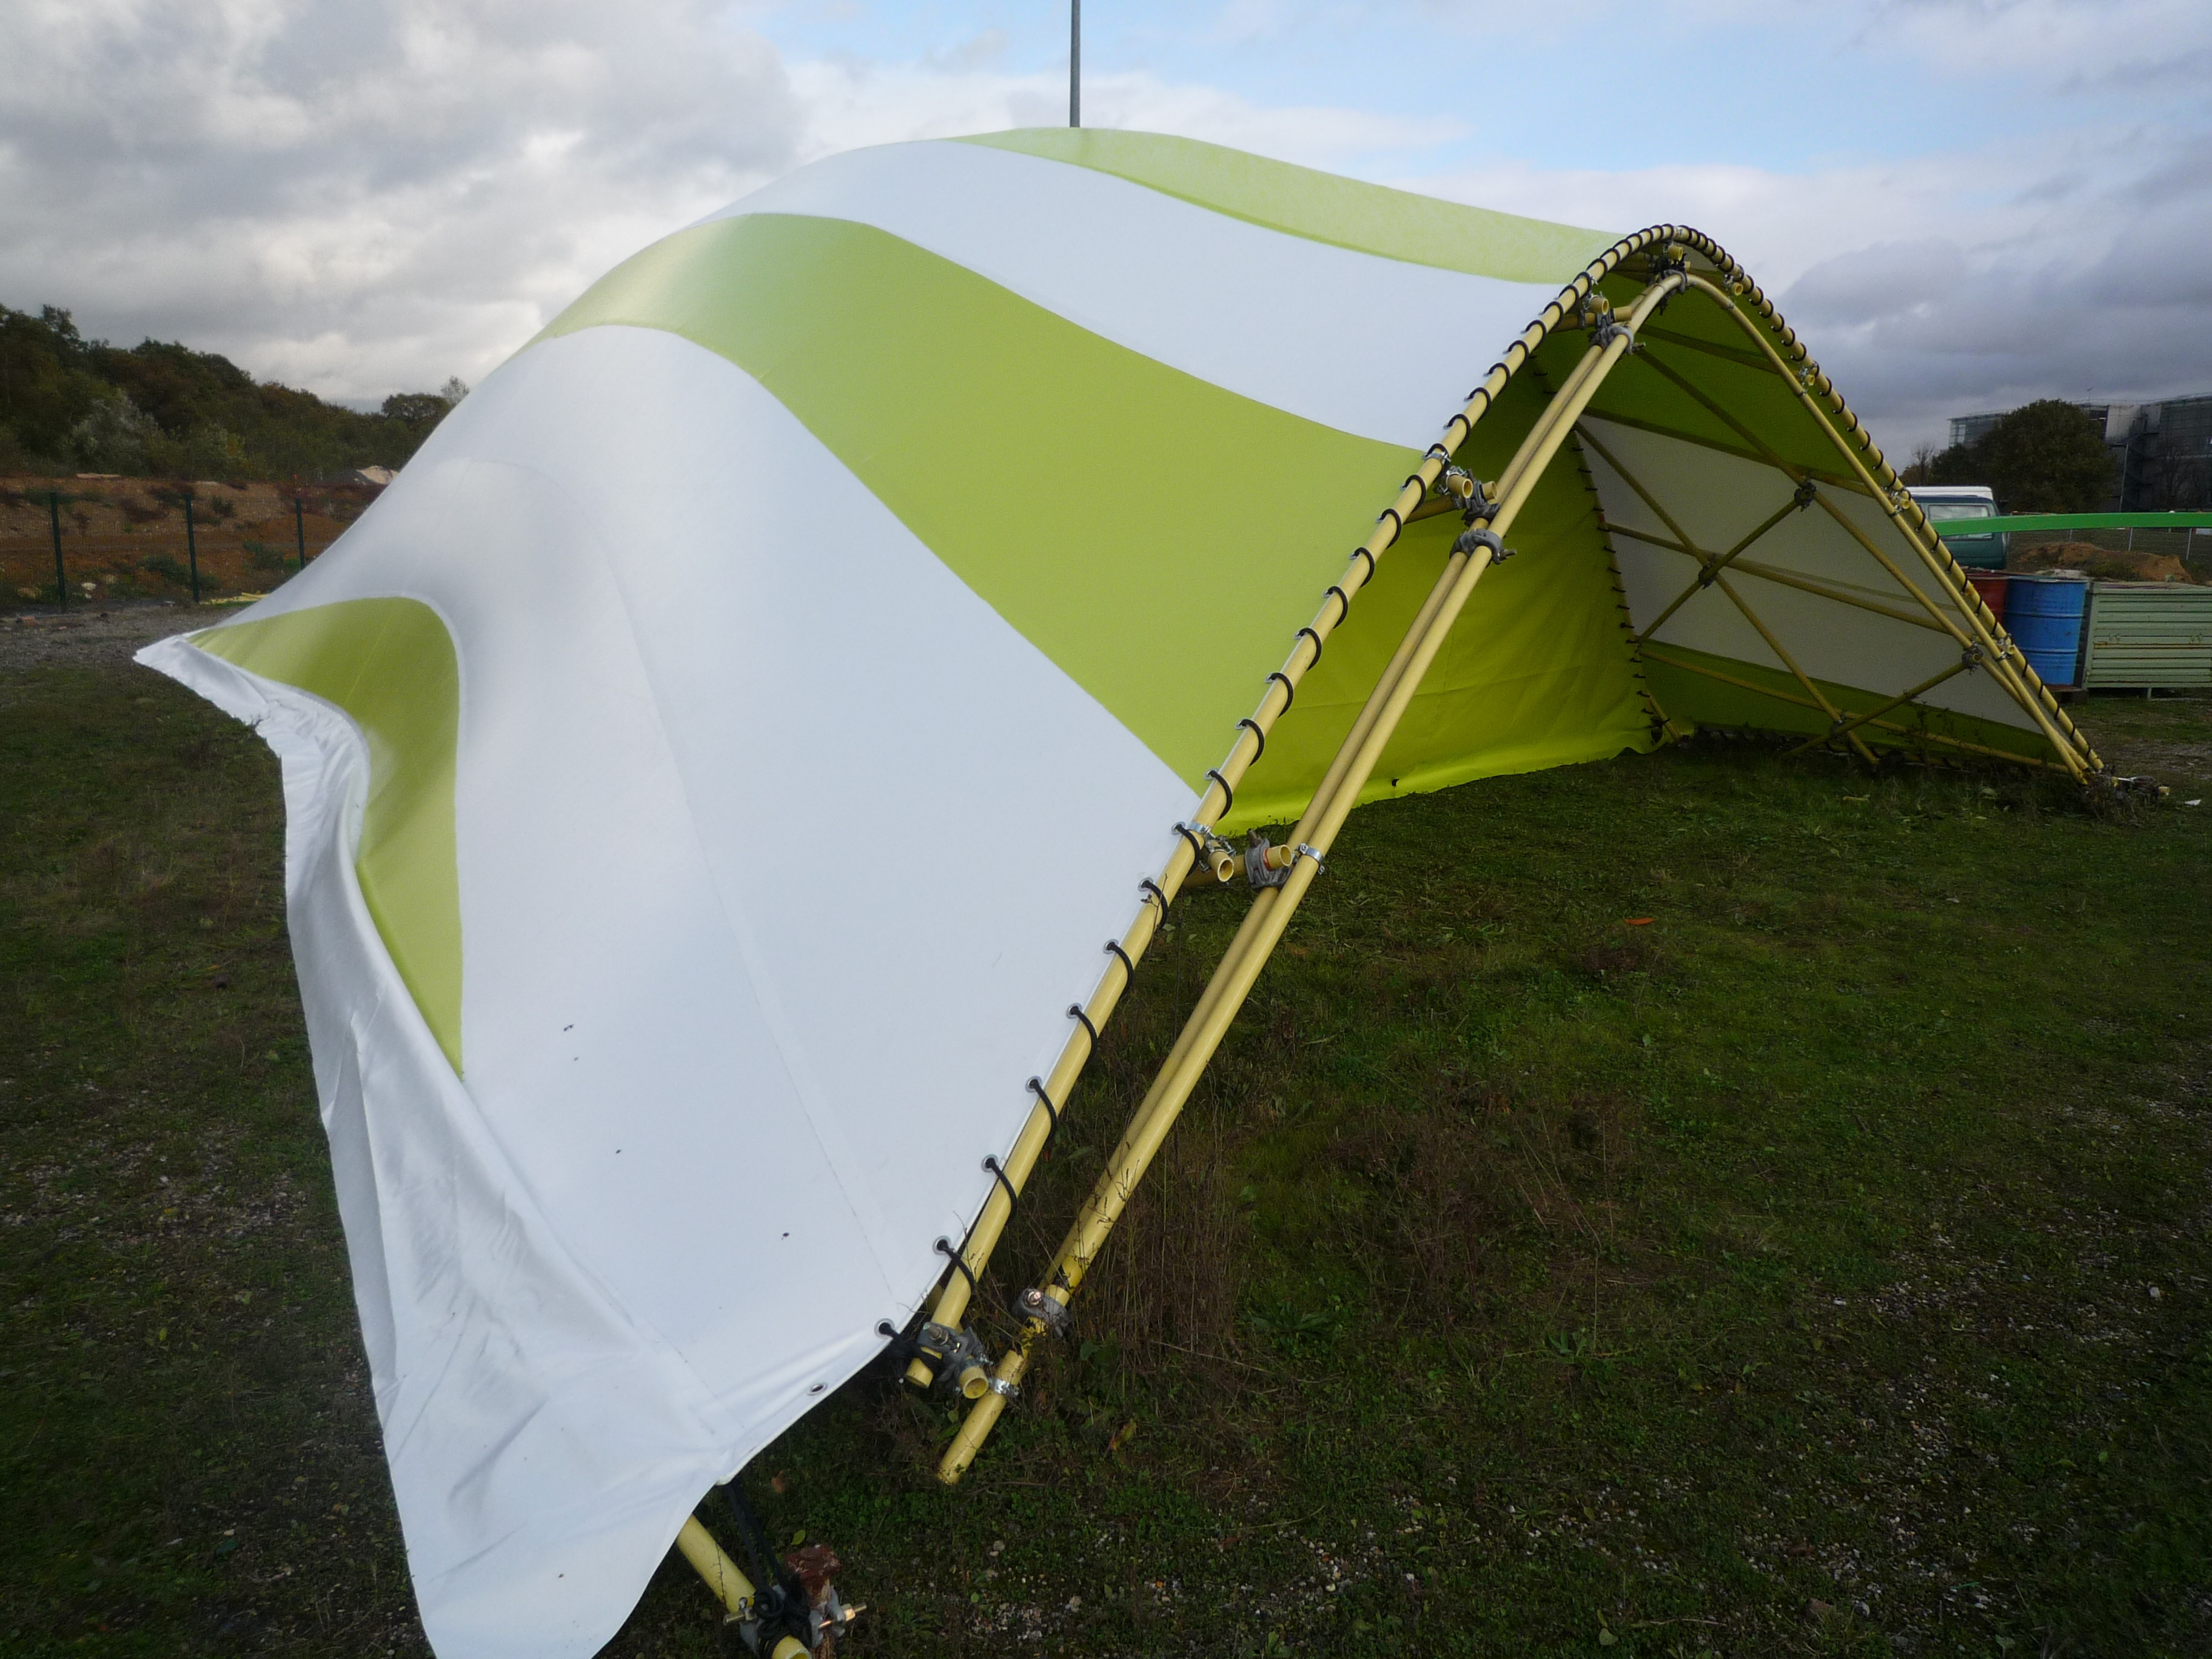
\includegraphics[width=0.48\textwidth]{proto_b.jpg}\label{fig:proto_a}}
		\hspace*{\fill}
		\subfloat[][Second prototype (2007)]{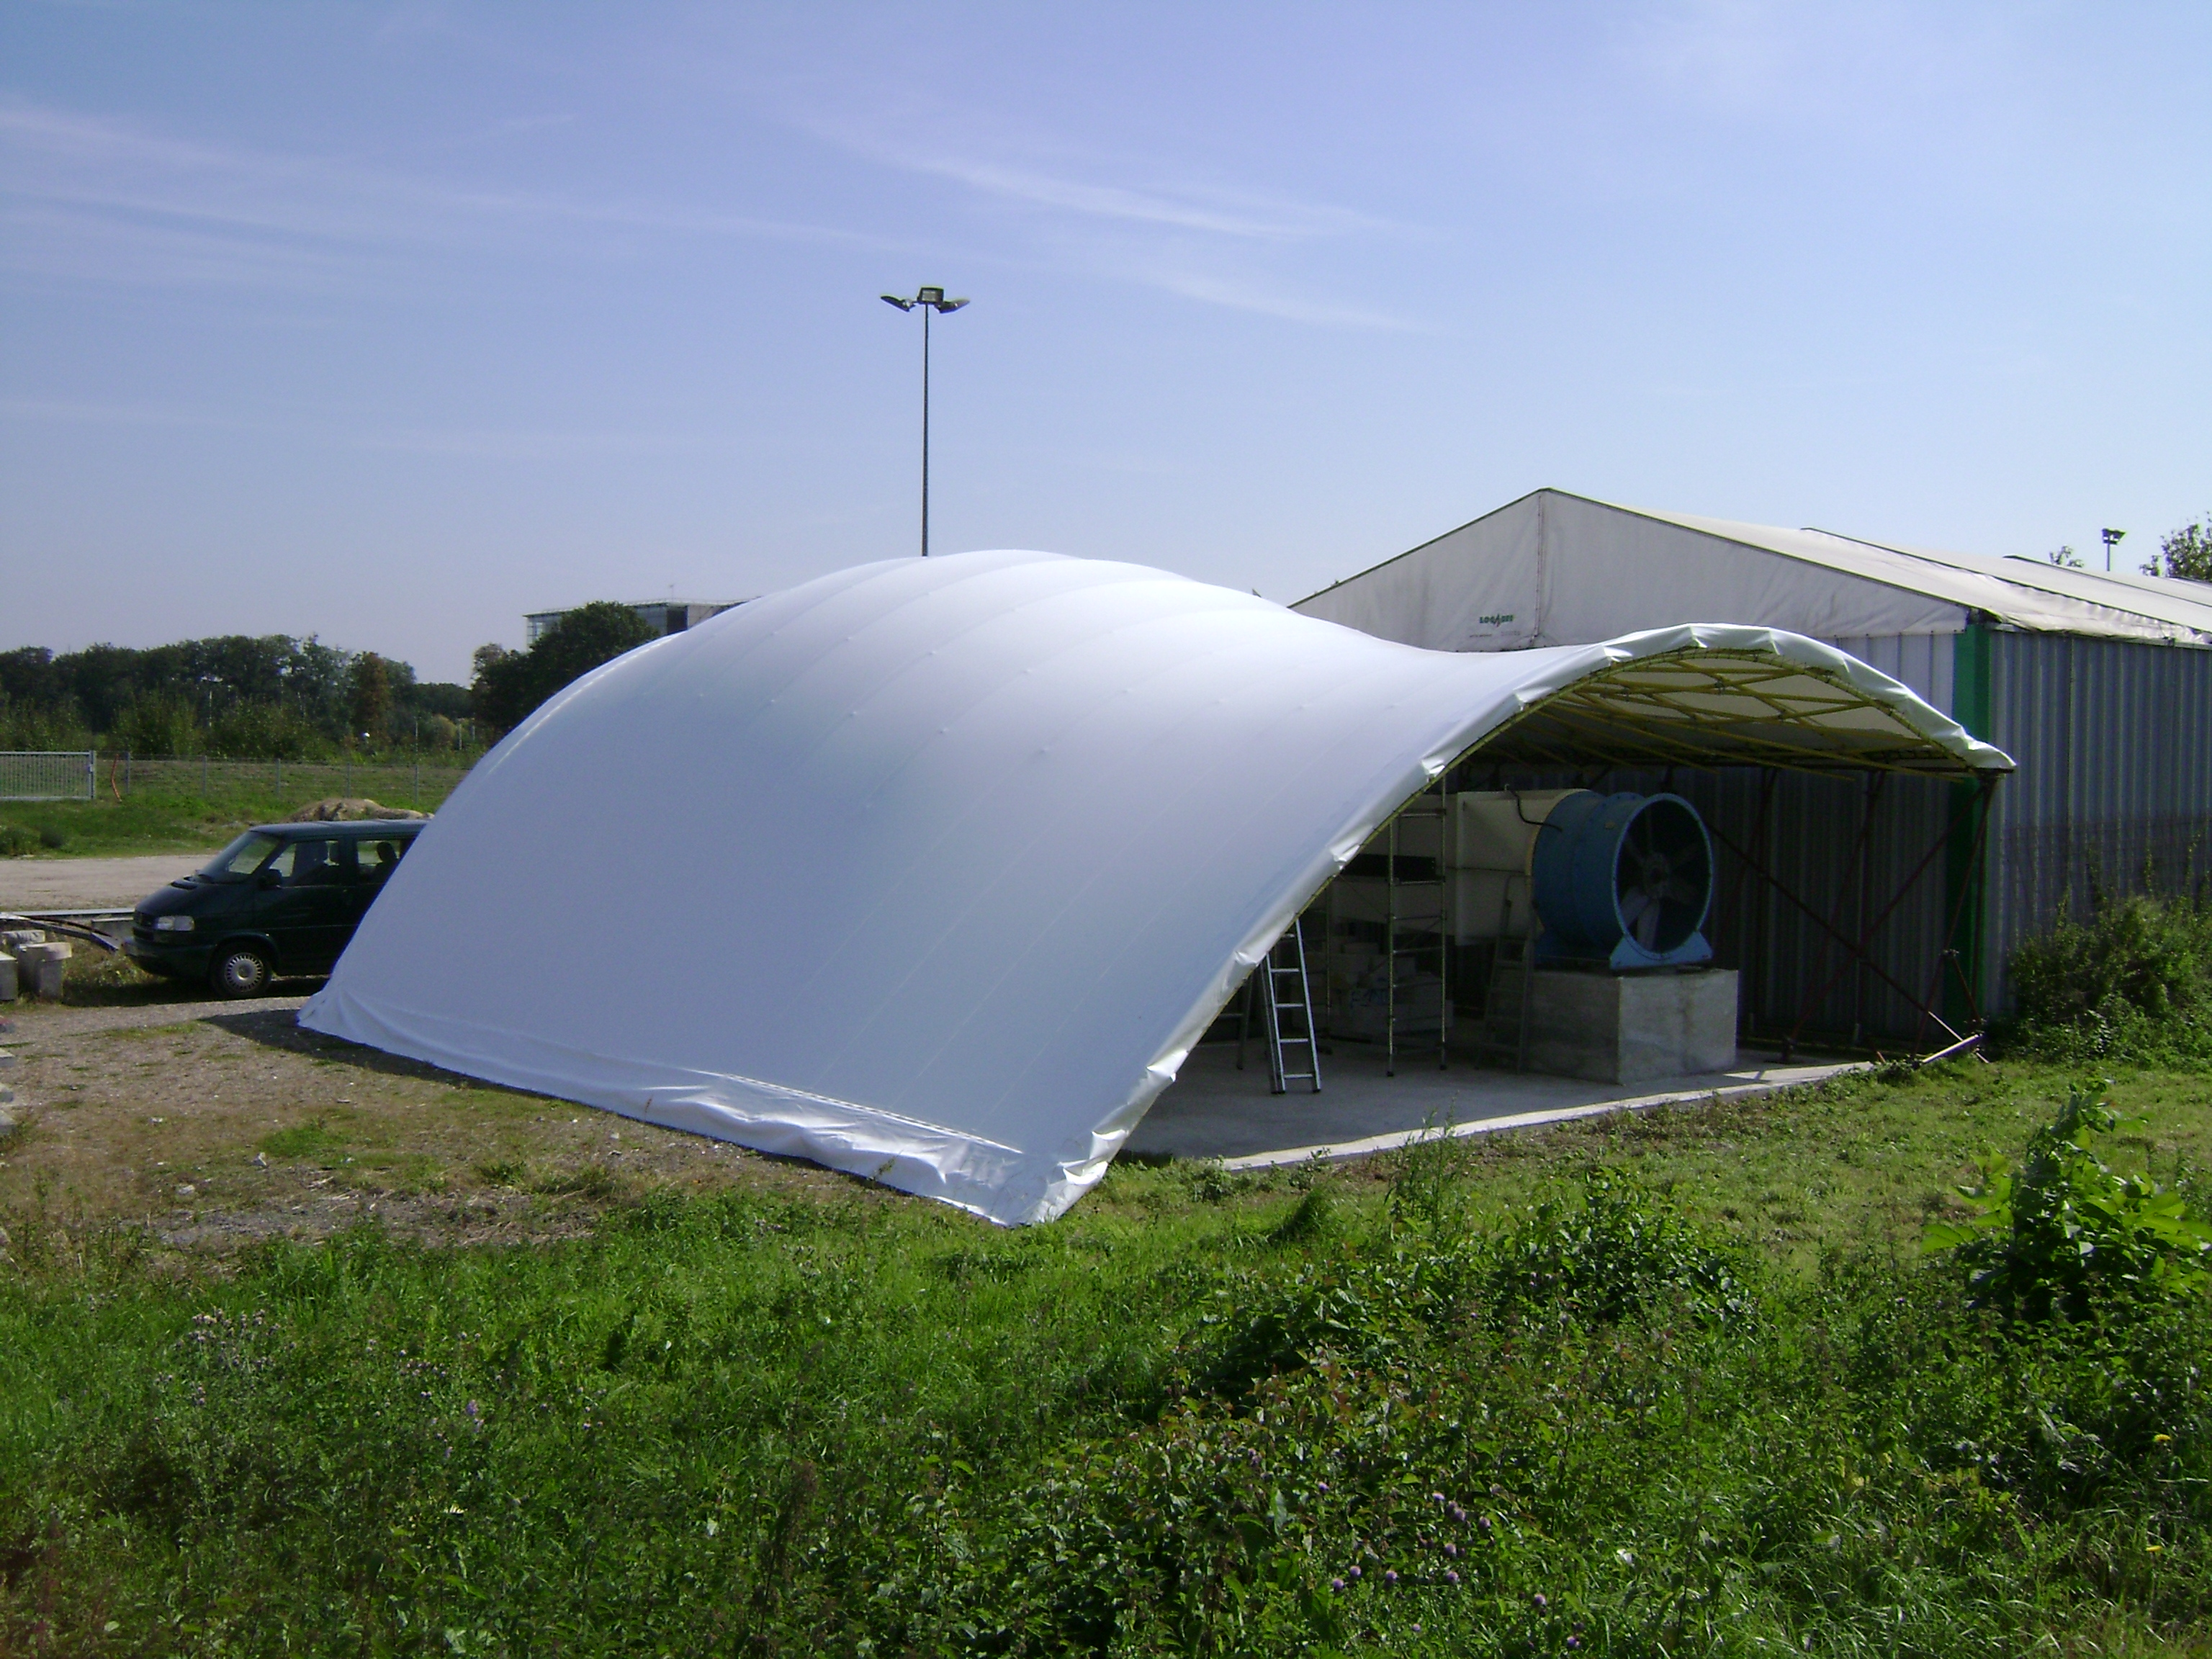
\includegraphics[width=0.48\textwidth]{proto_a.jpg}\label{fig:proto_b}}
		\vspace{10pt}
		\captionof{figure}[GFRP gridshell built in 2006 and 2007 in Noisy-Champs, France]{GFRP gridshell built in 2006 and 2007 in Noisy-Champs, France.}
		\label{fig:proto}
		%
		\vspace{0.5cm}
		%
		\subfloat[][Interior view]{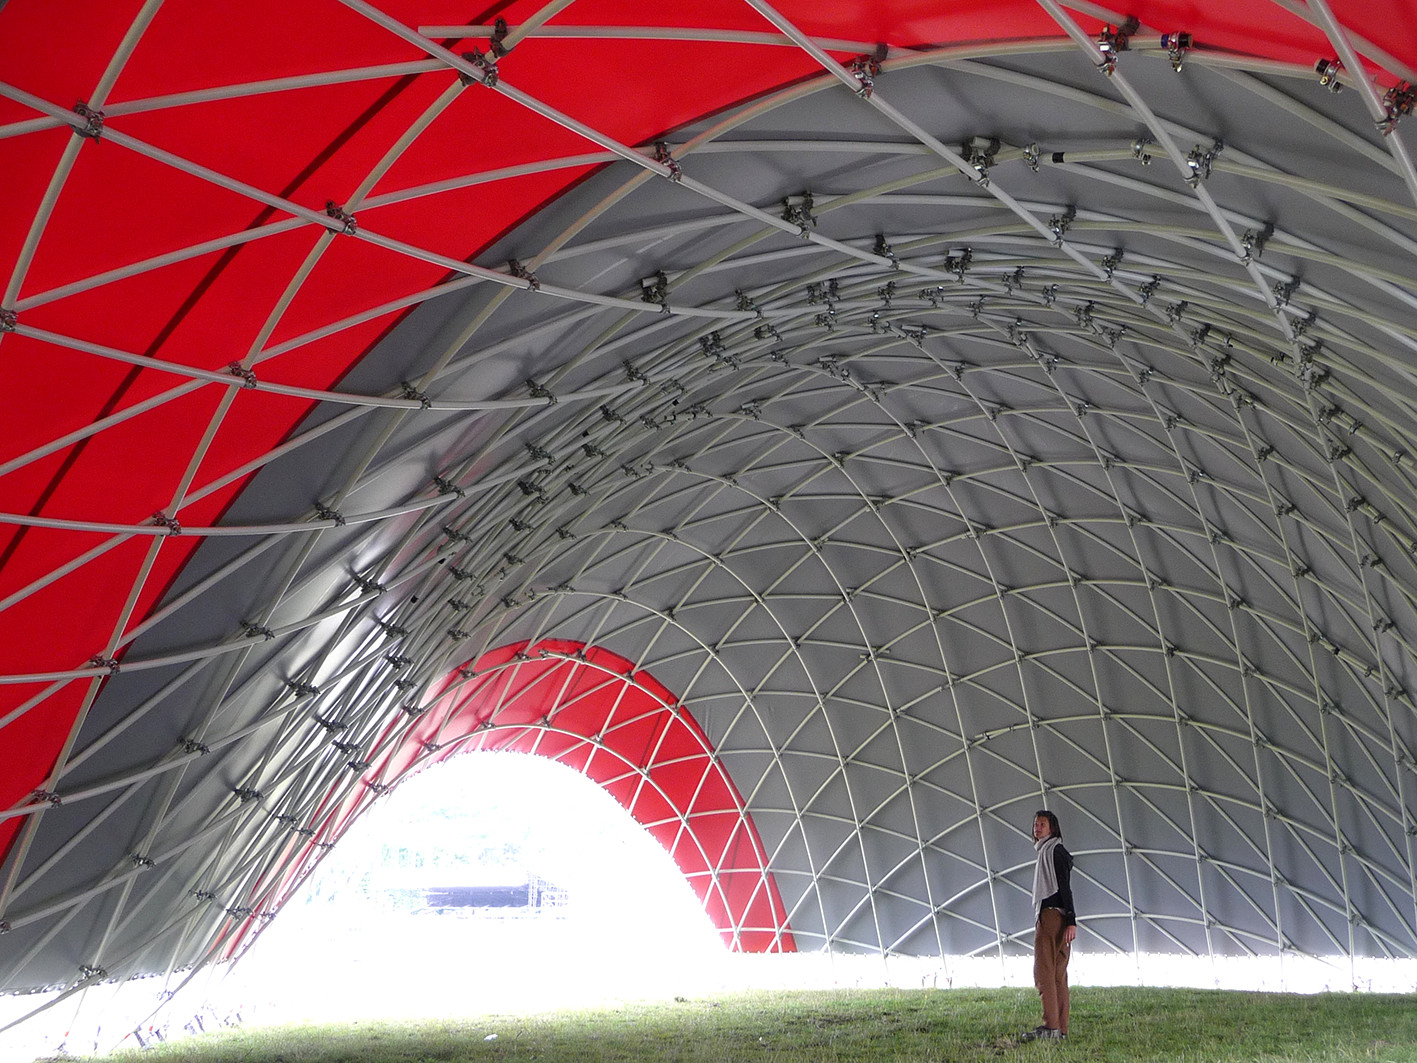
\includegraphics[width=0.48\textwidth]{solidays_int.jpg}\label{fig:solidays_a}}
		\hspace*{\fill}
		\subfloat[][Exterior view]{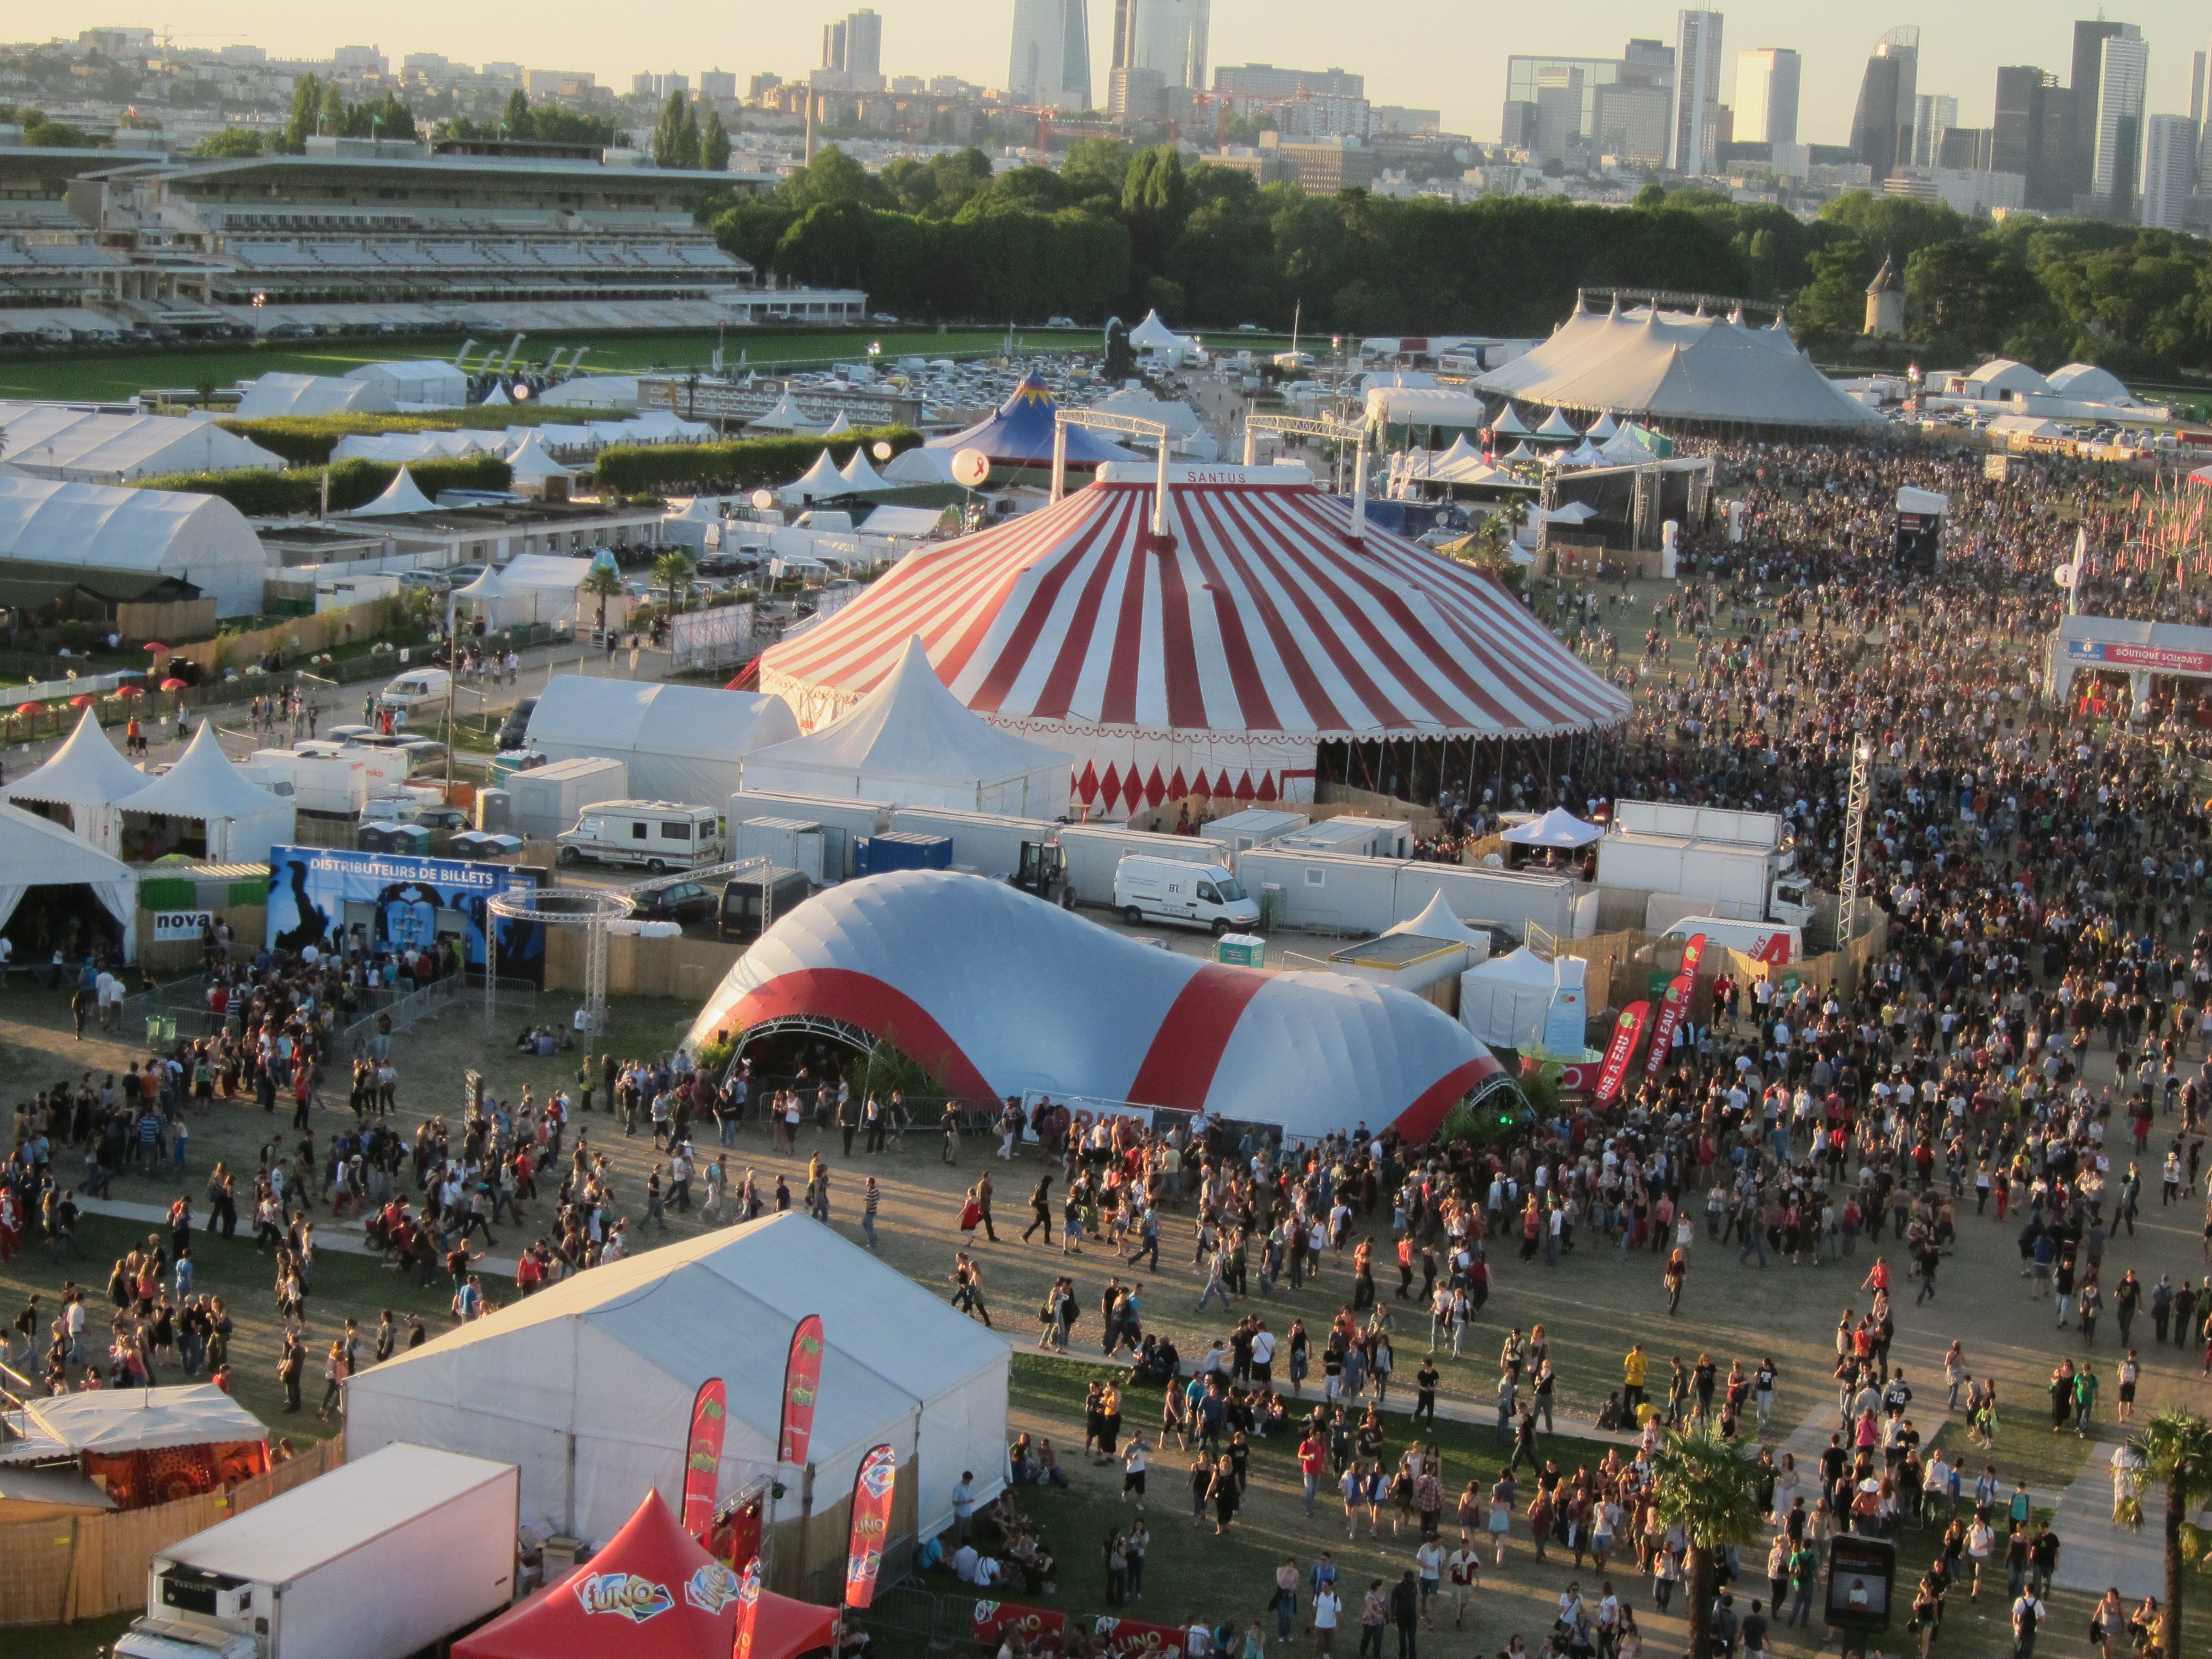
\includegraphics[width=0.48\textwidth]{solidays_ext.jpg}\label{fig:solidays_b}}
		\vspace{10pt}
		\captionof{figure}[Solidays GFRP gridshell built in 2011 in Paris, France]{Solidays GFRP gridshell built in 2011 in Paris, France.}
		\label{fig:solidays}
		%
		\vspace{0.5cm}
		%
		\subfloat[][Interior view]{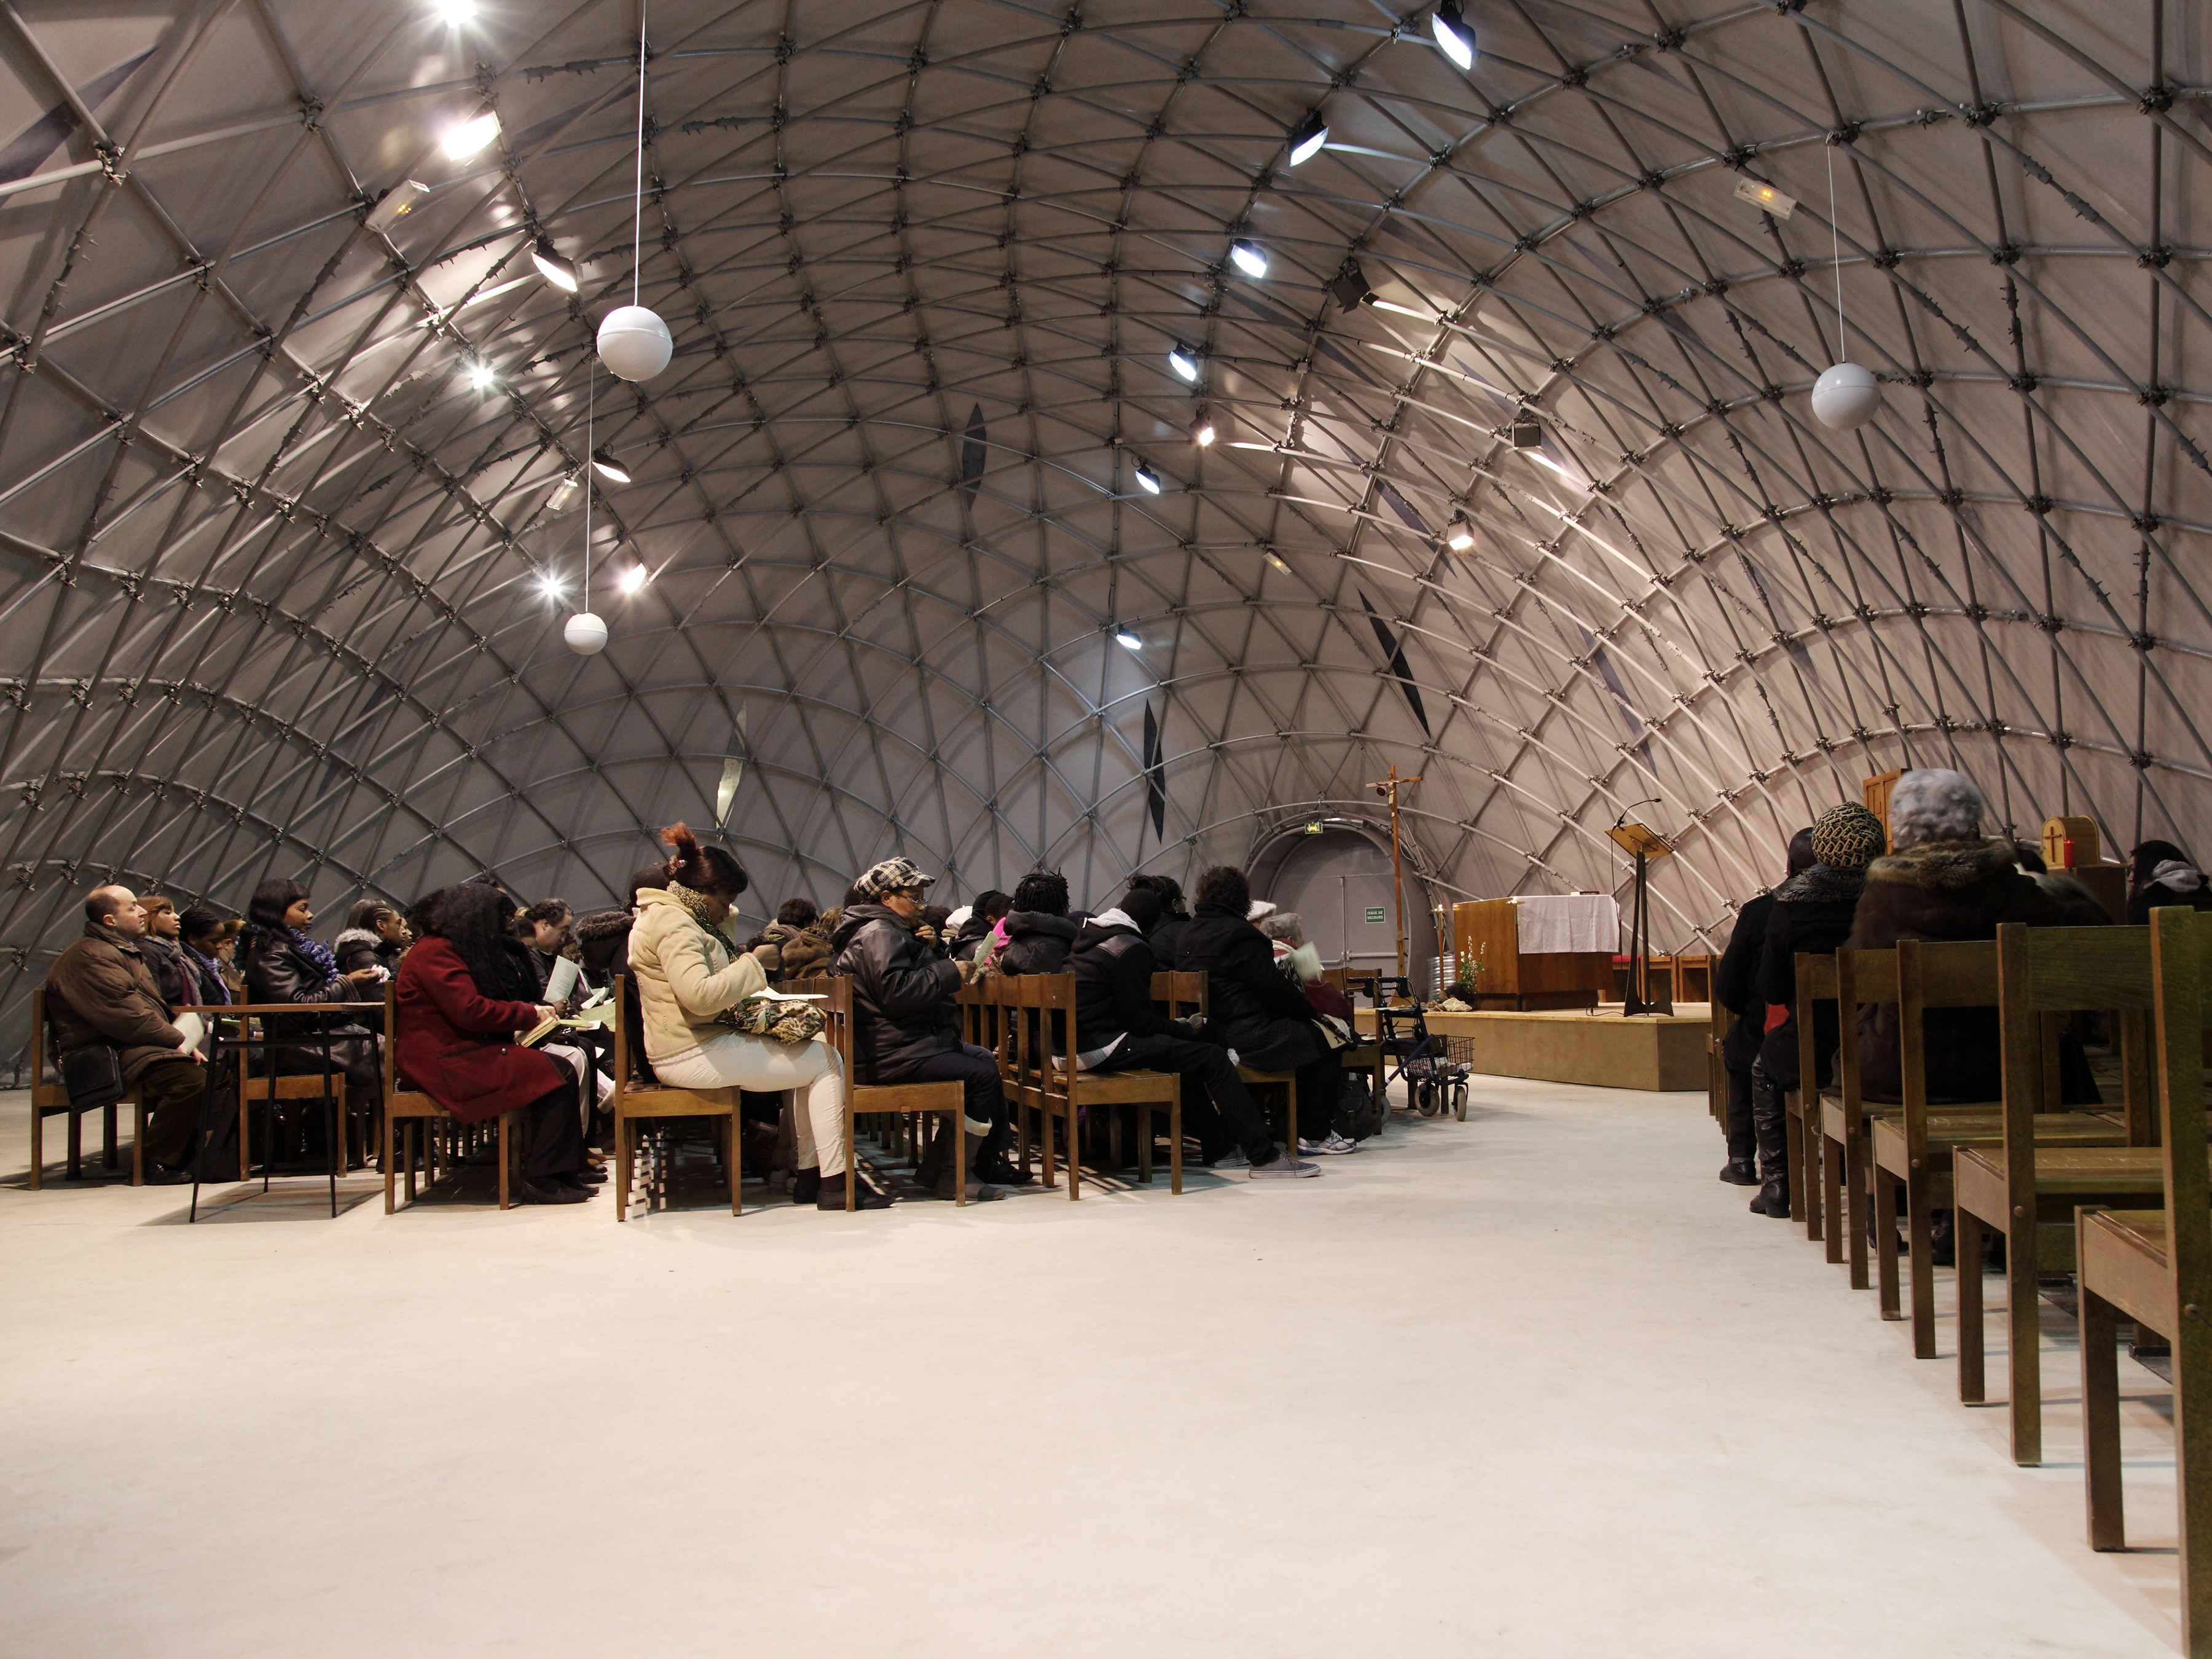
\includegraphics[width=0.48\textwidth]{creteil_int.jpg}\label{fig:creteil_a}}
		\hspace*{\fill}
		\subfloat[][Exterior view]{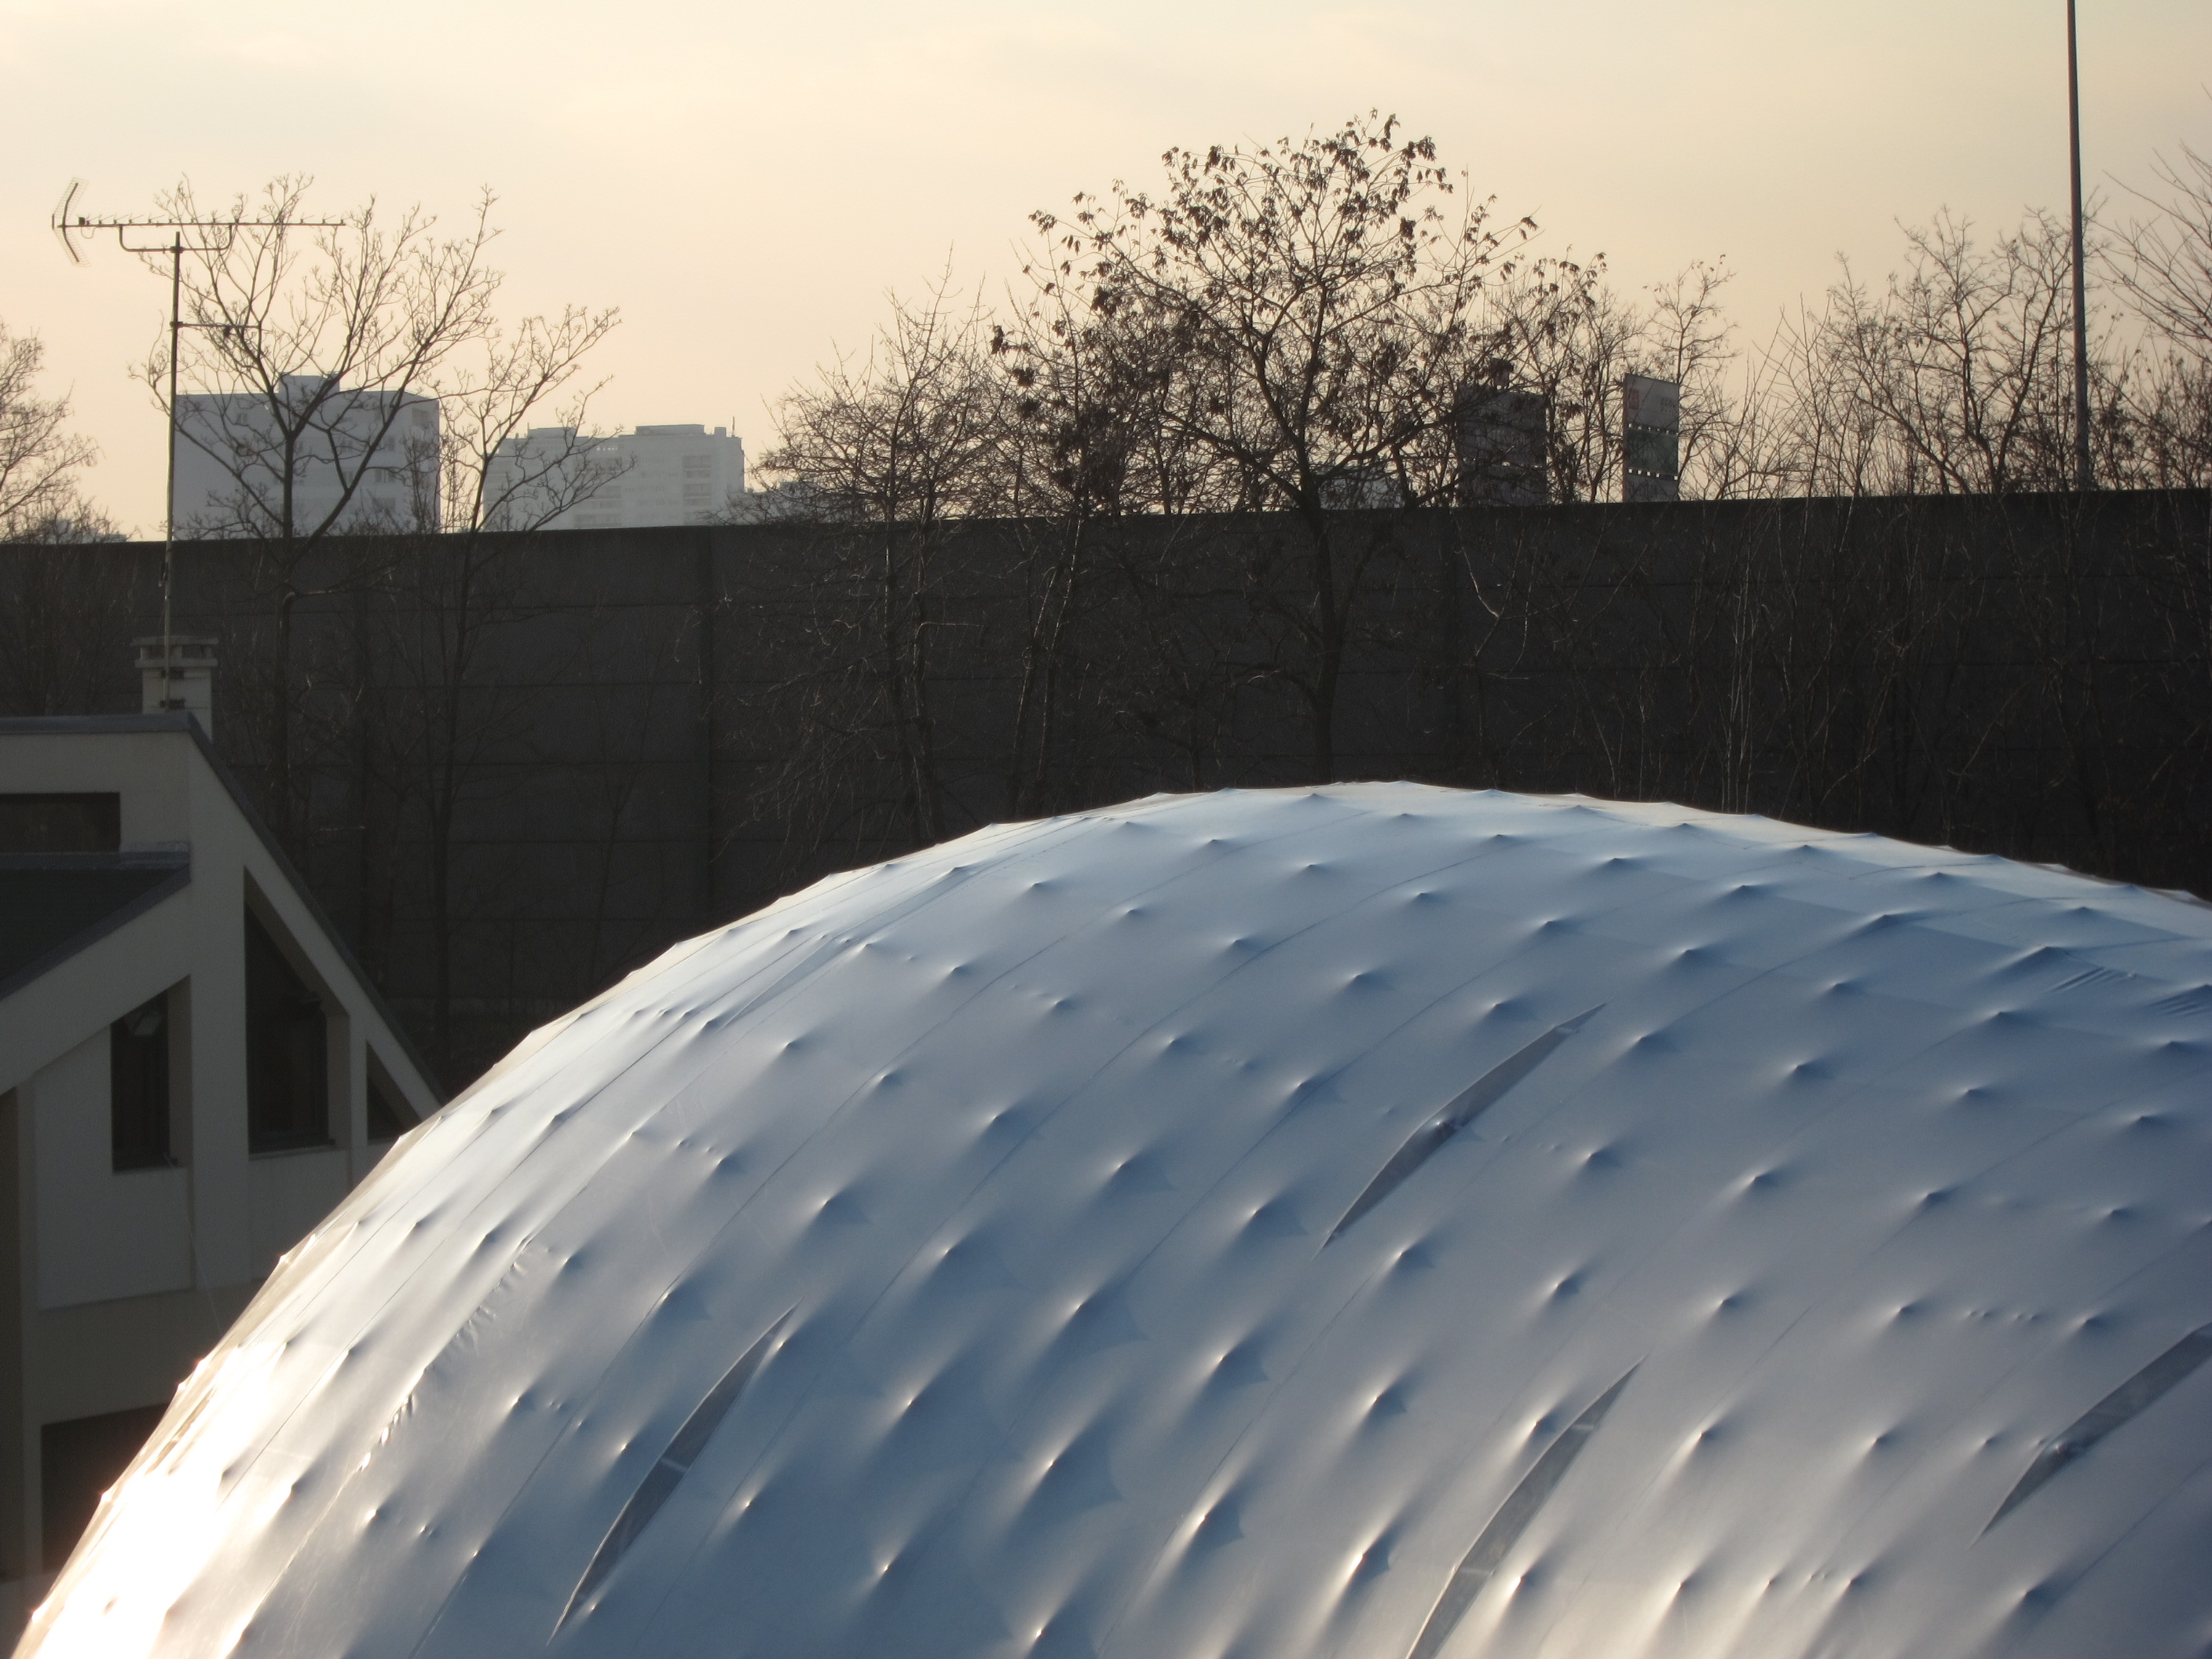
\includegraphics[width=0.48\textwidth]{creteil_ext.jpg}\label{fig:creteil_b}}
		\vspace{10pt}
		\captionof{figure}[GFRP gridshell built in 2013 in Créteil, France]{GFRP gridshell built in 2013 in Créteil, France.}
		\label{fig:creteil}
%	\end{fullpage}
\end{figure}

\subsubsection{Ephemeral Cathedral, Créteil, France, 2013}
The \emph{Ephemeral Cathedral} of Créteil is the last achievement of this kind \cite{DuPeloux2016}.\footnote{Photos and videos of the construction process at : \url{http://thinkshell.fr/gridshell-cathedral-2013/}} It was designed by \href{http://www.tess.fr}{T/E/S/S} (L. du Peloux, B. Vaudeville, T. Gray, S. Aubry) with the assistance of \href{http://navier.enpc.fr}{Navier} (F. Tayeb, J-F. Caron, O. Baverel, A. Tamaint).\footnote{For this project, I was in charge of the project development for T/E/S/S, including structural and technical design, detailing, doors, membrane, drawing production, fabrication and erection with the help of the parishioners, regulations, \telp{}}. This time, the structure is a real building meant to last a decade and is still in activity since its construction in 2013. A complete review of this project is given in the next chapter of this thesis (see \cref{chp=creteil}).

The single-layer gridshell covers about \SI{350}{m^2} and spans 17 meters (see \cref{fig:creteil_a}). It is covered by a PVC coated fabric membrane (see \cref{fig:creteil_b}). It was erected by two mobile cranes.


\subsection{Flourishing timber gridshell pavilions}
Since 2010, about 20 timber gridshell pavilions were built around the world, mainly during workshops. Here, we do not review all of these pavilions in detail because they are quite similar although each one has its specificities.

\subsubsection{The impetus given by gridshell.it}
Around 2010, a research group gathering architectural and engineering skills appeared under the name \href{http://www.gridshell.it}{gridshell.it} in Italy. Inspired by the work of Frei Otto, they revisited the structural system developed at Mannheim and adapted it to a range of small-scale timber pavilions.

These pavilions have in common to be double-layer timber gridshells. The structural system is always composed of laths with rectangular cross-section. The laths come in short length  from the sawmill (about 3 to 4 meters). They do not try to re-form long-length laths with complex jointing techniques. Instead, they use a simple splice system. Although it is not well architecturally resolved, it is efficient enough for this kind of project. As the laths are short, this detail is repeated frequently in the grid, but the splice system enable a higher level of prefabrication of the grid. Thus, small modules of the size of the laths can be preassembled and connected with the splice system to re-form the full grid. These gridshells are braced either with cables or with individual diagonal members in each cell.

These structures were never meant to provide full waterproofness although some were an occasion to experiment different types of cladding with boards (Lecce 2010, Toledo 2012, Milano 2013) or with textile membranes (Lecce 2009).

One of their first pavilion was built in 2010 in Lecce, Italy (see \cref{fig:lecce}). Their most known project is probably the Toledo pavilion built in 2012 in Naples, Italy.  A new pavilion called Toledo 2.0 was built in 2014 in Naples, Italy (see \cref{fig:toledo2}). Although it seems that their initial approach focused more on the architectural aspects and the construction process, they rapidly tried to develop dedicated computer design methods \cite{DAmico2014} and did significant wood testing \cite{DAmico2015a}.

\subsubsection{Other similar timber pavilions}
The ideas of the \emph{gridshell.it} group spread rapidly and similar projects were achieved outside of Italy. Amongst them, we can point out the ZA pavilion built in 2013 in Cluj, Romania \cite{Naicu2014}; the F\textsuperscript{2} pavilion built in 2014 in San Antonio, USA, with an interesting folding skin (see \cref{fig:sanantonio,fig:sanantonio2}) and the pavilion built in 2016 in Trondheim, Norway, which is made of very short length laths spliced every two cells \cite{Mork2016,Labonnote2016}.

\begin{figure}[p]
     	\centering
%	\begin{fullpage}
		\subfloat[][Lecce, 2010]{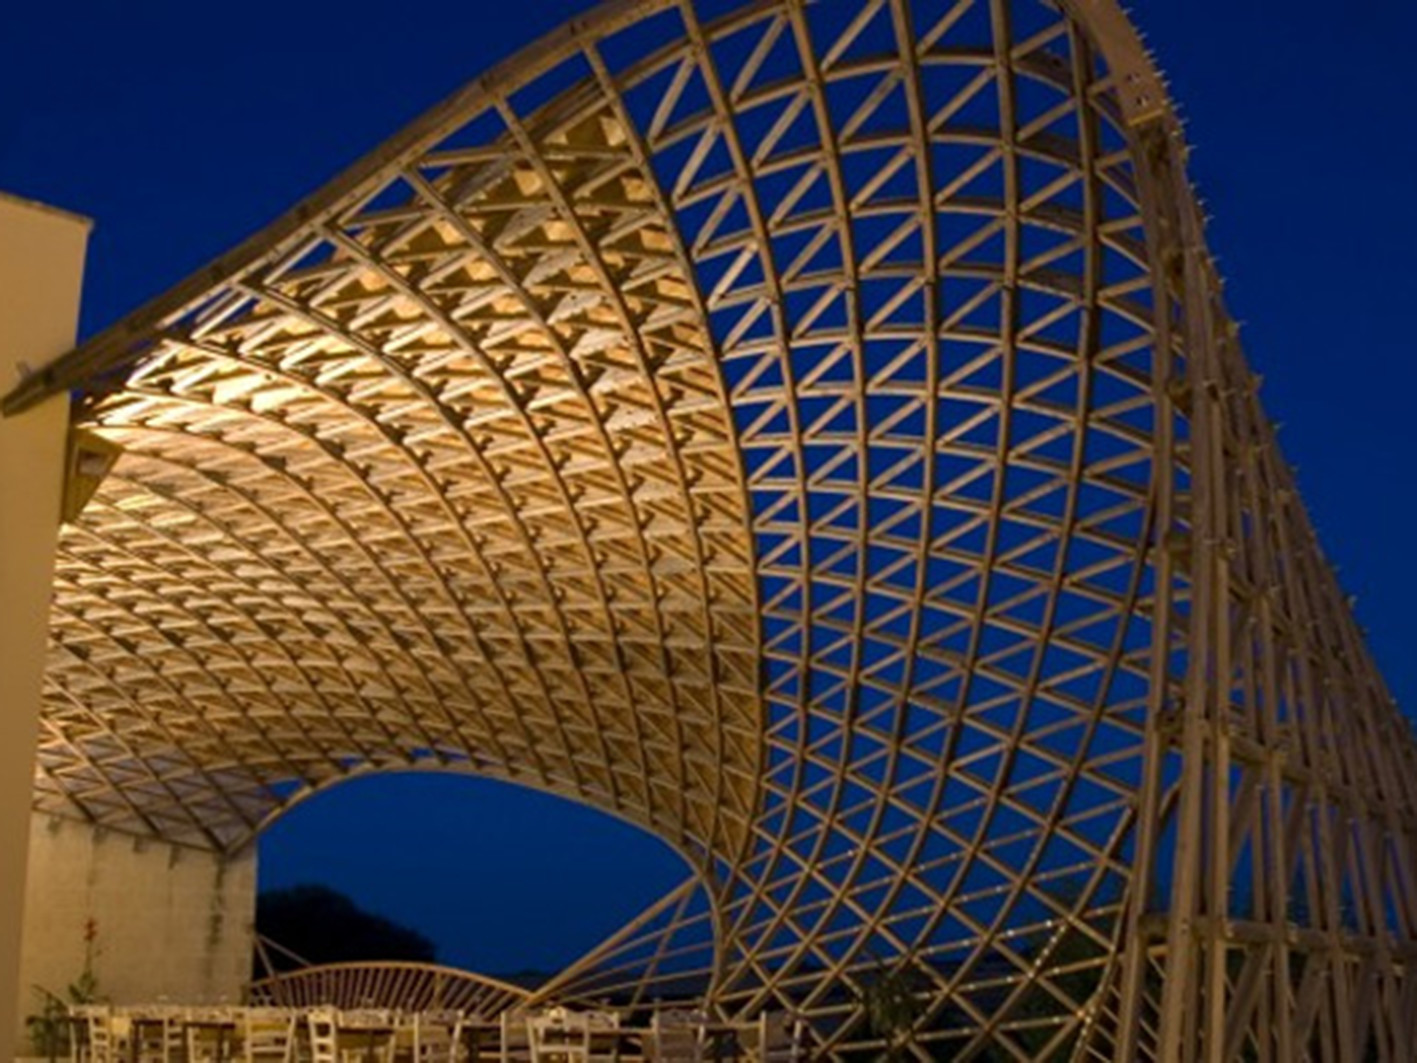
\includegraphics[width=0.48\textwidth]{lecce.jpg}\label{fig:lecce}}
		\hspace*{\fill}
		\subfloat[][Toledo 2.0, 2014]{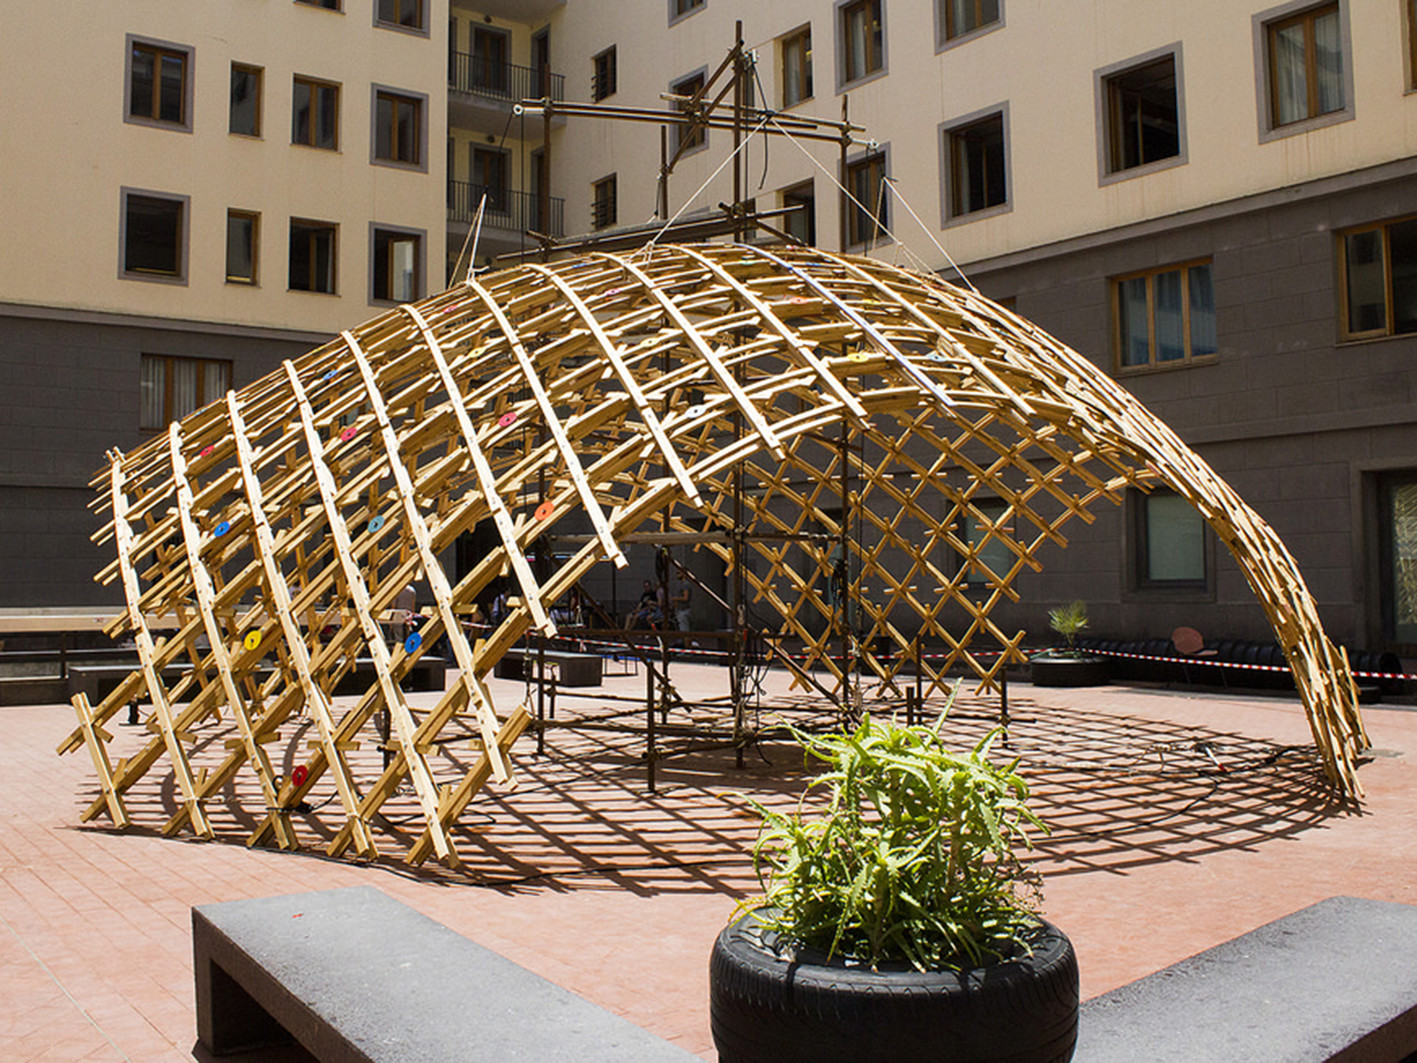
\includegraphics[width=0.48\textwidth]{toledo2.jpg}\label{fig:toledo2}}
		\vspace{10pt}
		\captionof{figure}[Timber gridshells built by gridshell.it in Italy]{Timber gridshells built by gridshell.it in Italy.}
		\label{fig:gsii}
		%
		\vspace{0.5cm}
		%
		\subfloat[][Folding skin]{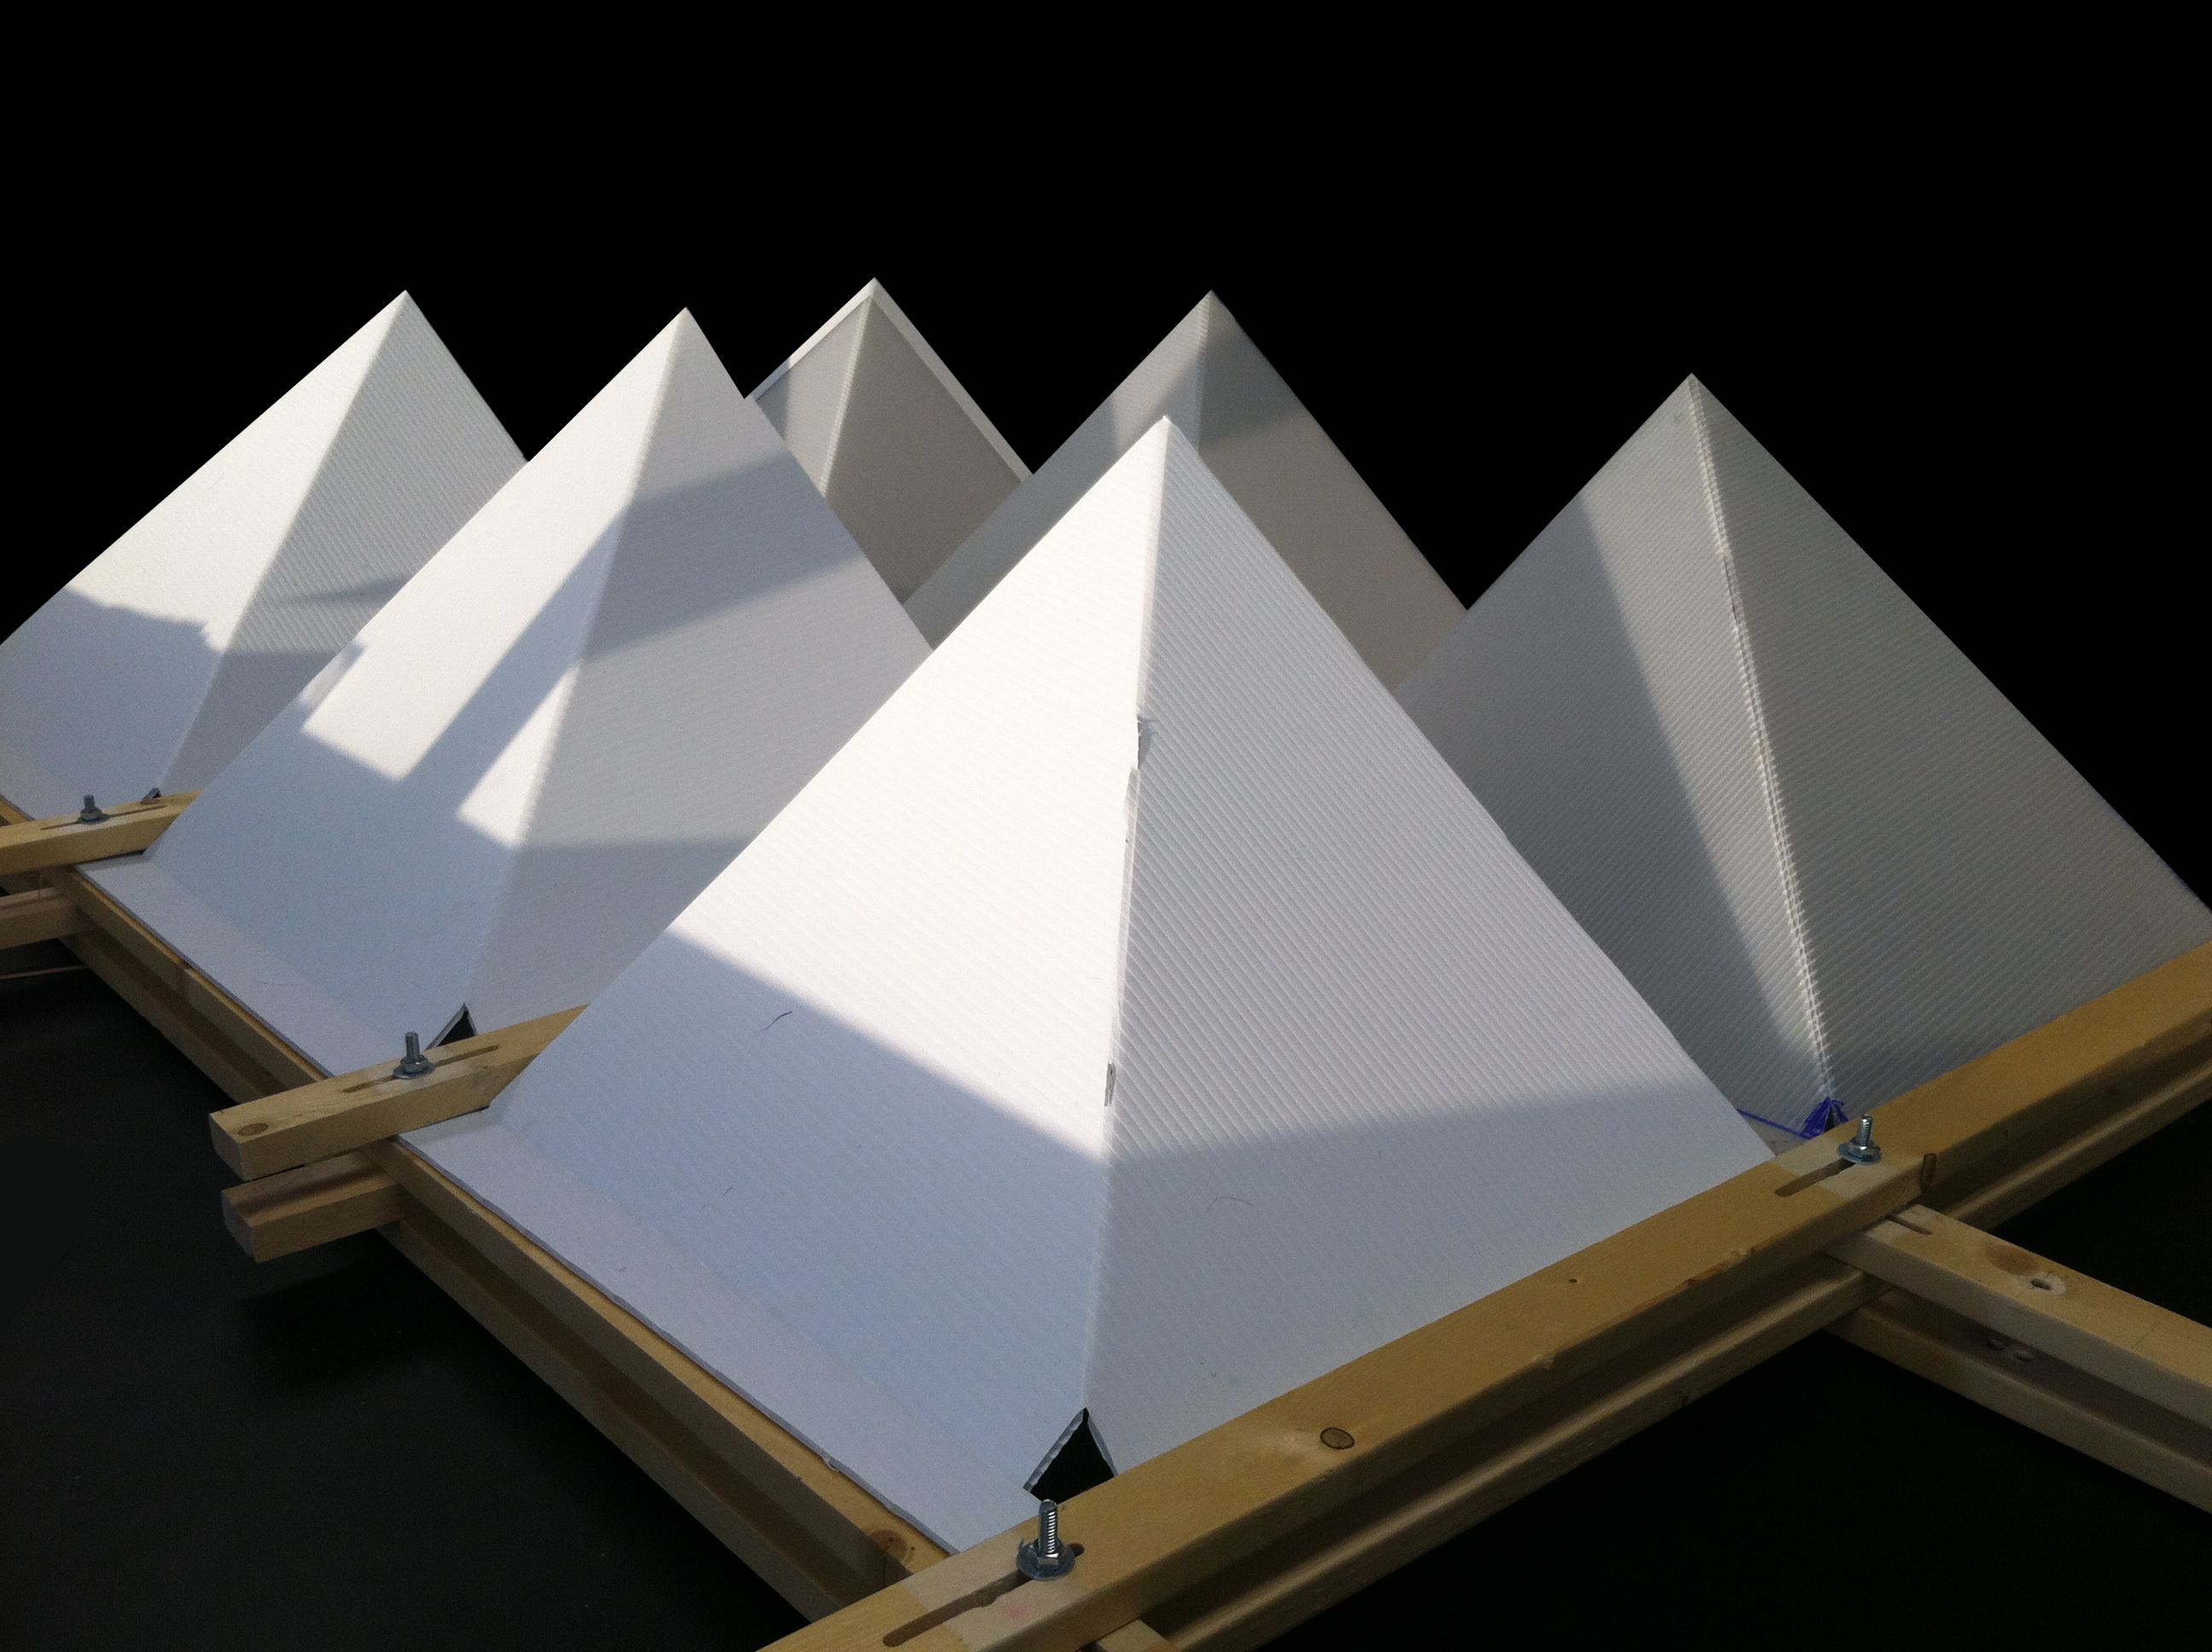
\includegraphics[width=0.48\textwidth]{sanantonio2.jpg}\label{fig:sanantonio2}}
		\hspace*{\fill}
		\subfloat[][Pavilion]{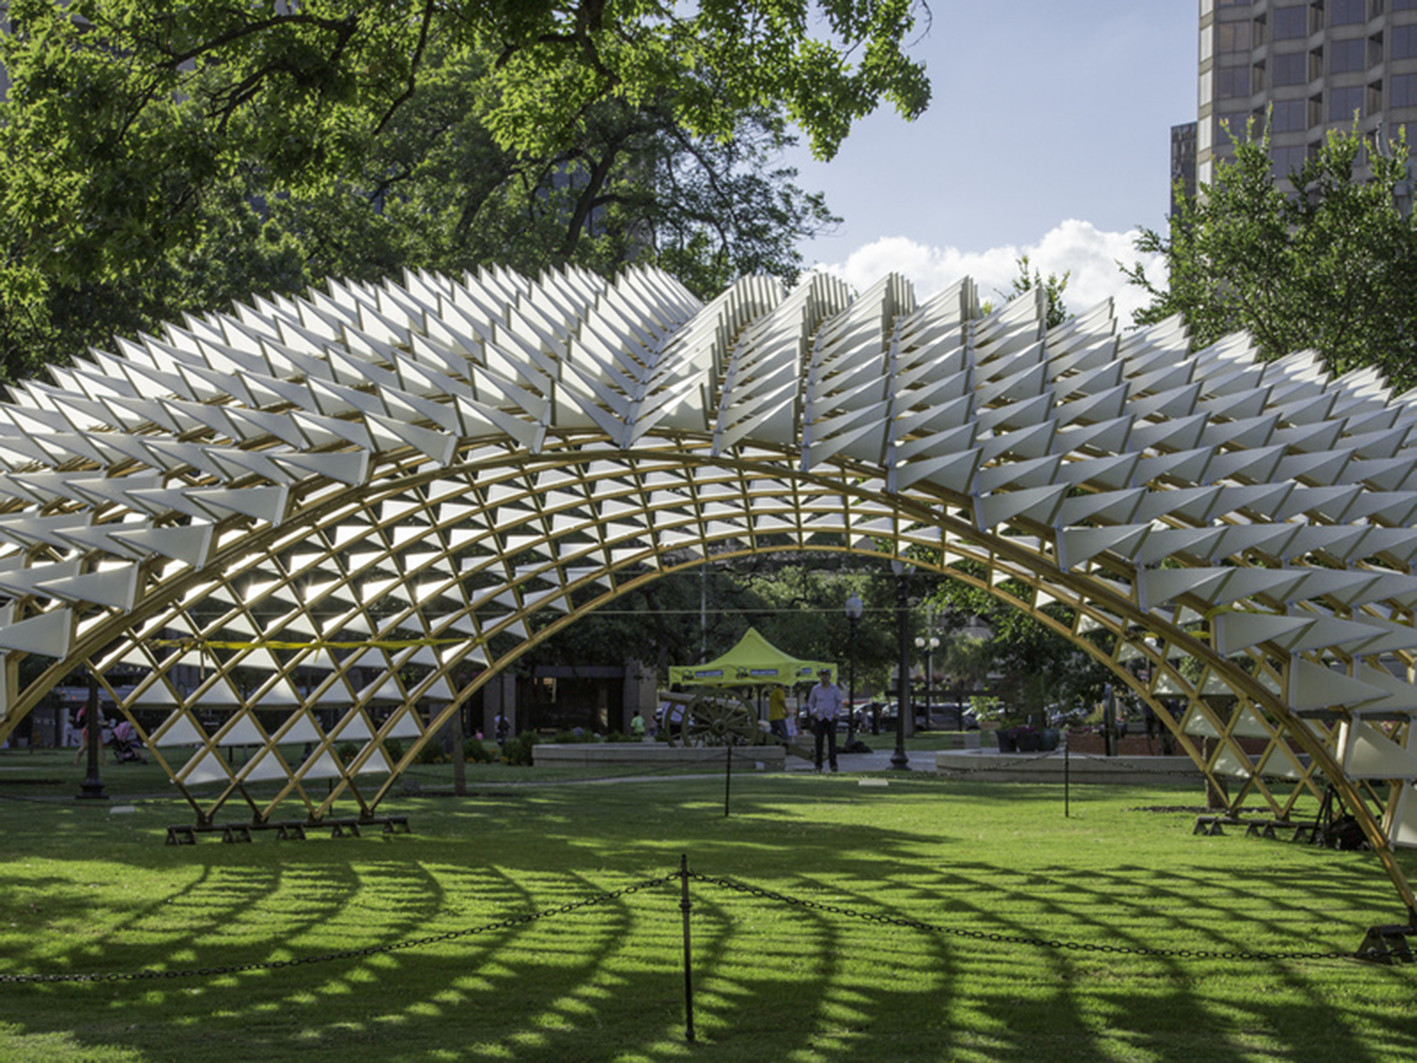
\includegraphics[width=0.48\textwidth]{sanantonio.jpg}\label{fig:sanantonio}}
		\vspace{10pt}
		\captionof{figure}[Timber gridshell built in 2013 in San Antonio, USA]{Timber gridshell built in 2013 in San Antonio, USA.}
		\label{fig:otherpav}
		%
		\vspace{0.5cm}
		%
		\subfloat[][Tensioner]{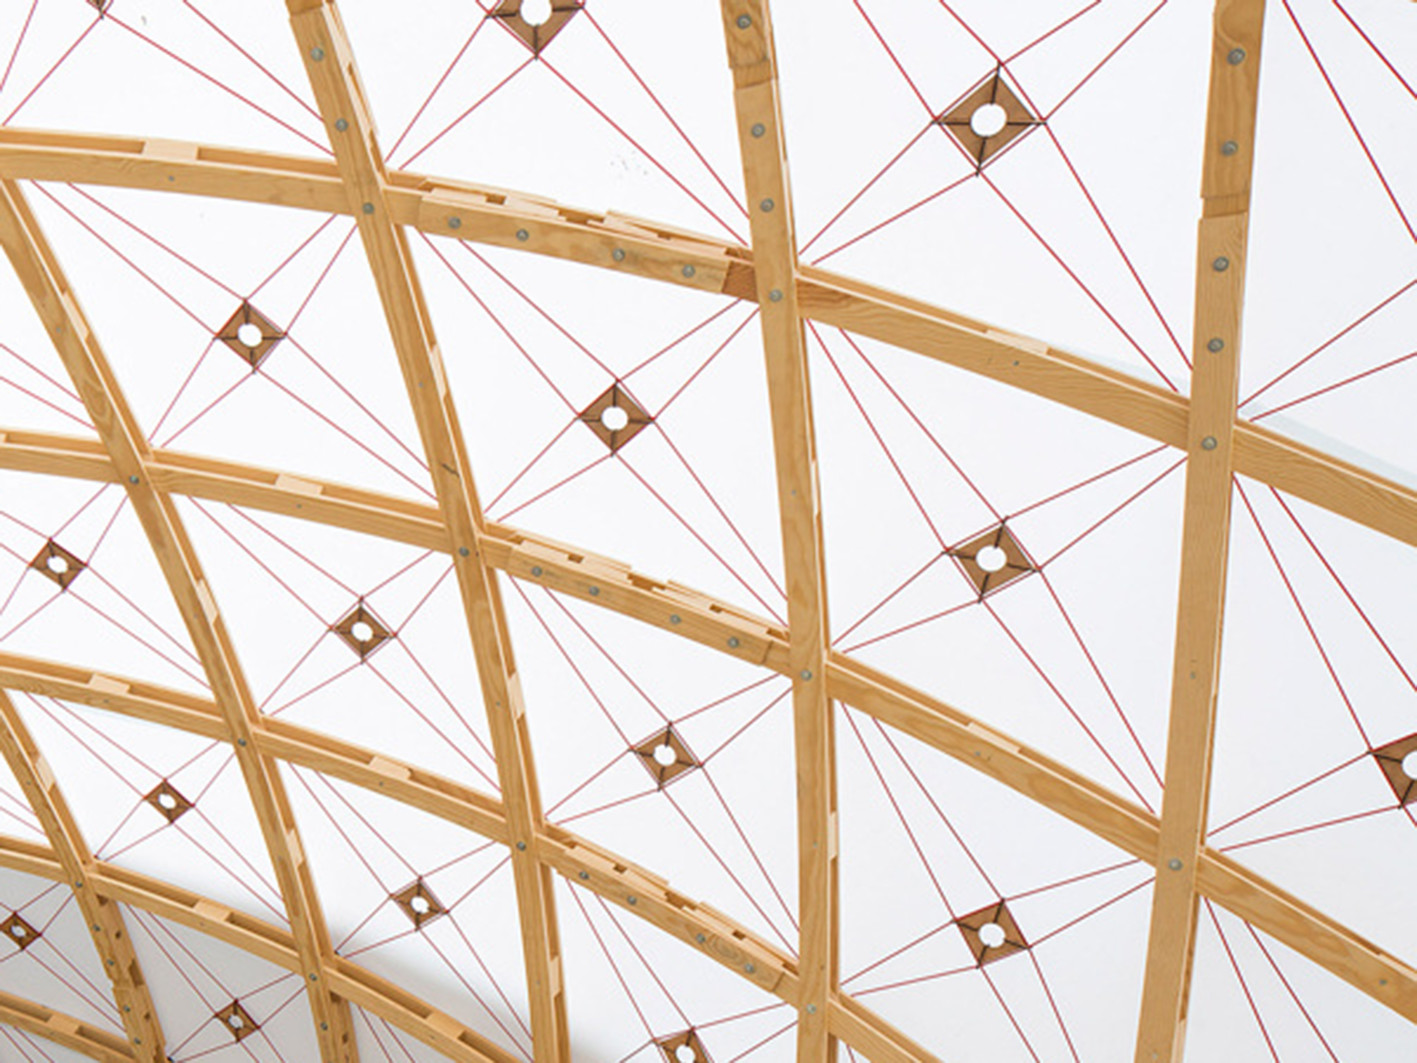
\includegraphics[width=0.48\textwidth]{montpellier2.jpg}\label{fig:tensioner}}
		\hspace*{\fill}
		\subfloat[][Pavilion]{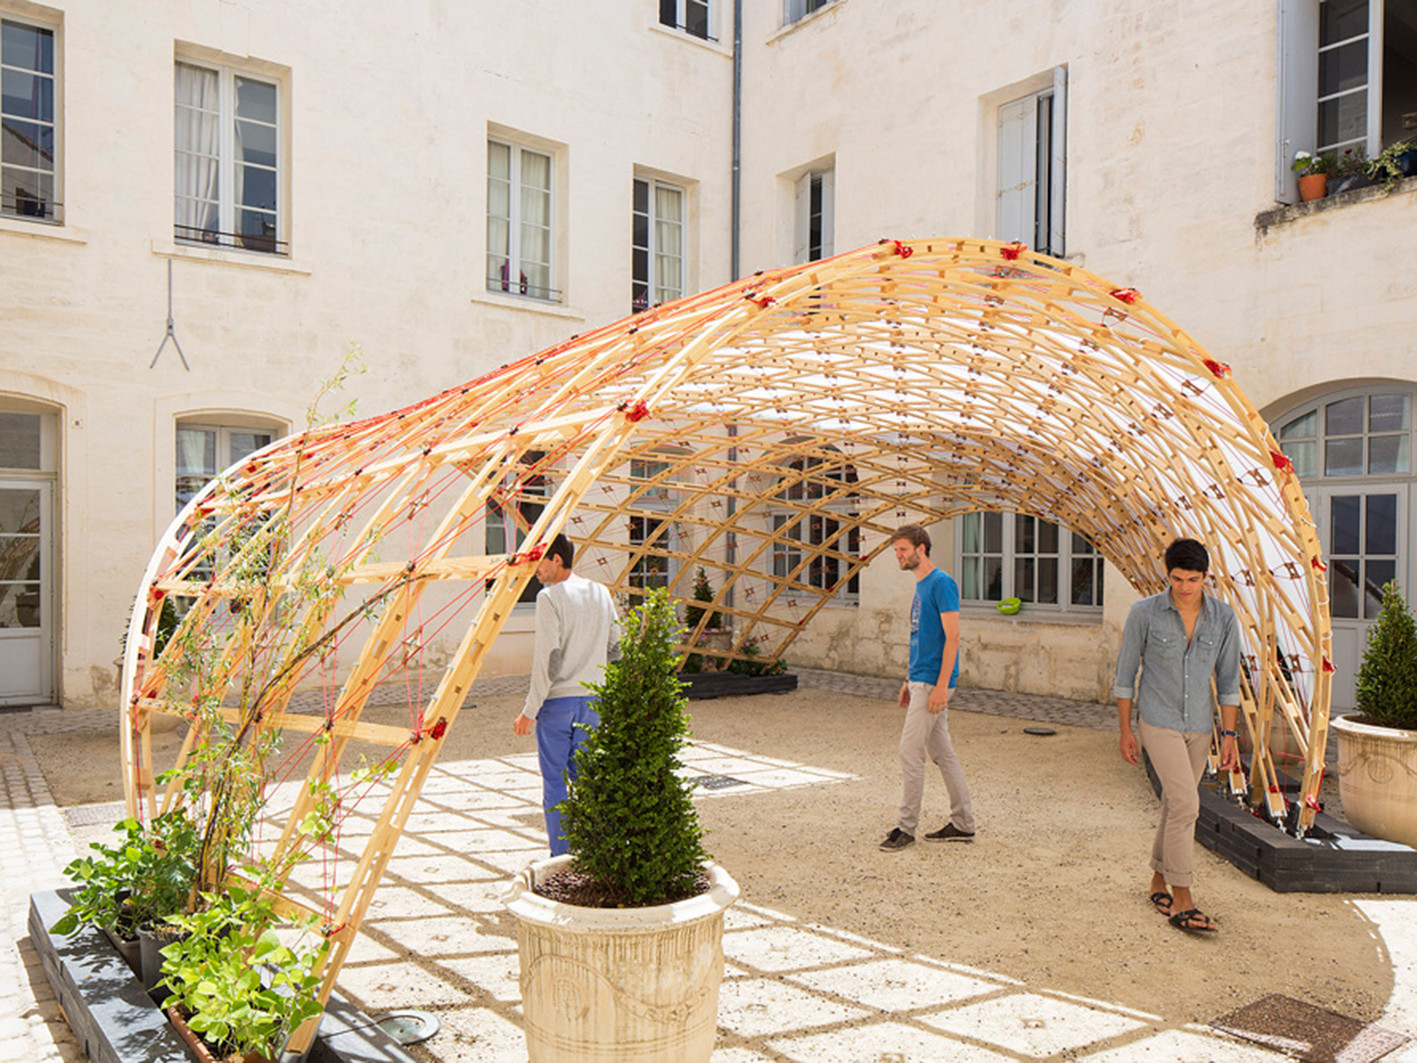
\includegraphics[width=0.48\textwidth]{montpellier.jpg}\label{fig:montpellier}}
		\vspace{10pt}
		\captionof{figure}[Timber gridshell built in 2016 in Montpellier, France]{Timber gridshell built in 2016 in Montpellier, France.}
		\label{fig:jpofav}
%	\end{fullpage}
\end{figure}

\subsubsection{Specific inputs from the laboratory Navier}
In that vein, L. du Peloux from \href{http://navier.enpc.fr}{Navier} and G. Laurent from \href{http://terrellgroup.net/index.php}{Terrell} helped two students (S. Hulin and G. Sudres) resp. from the \href{http://www.grenoble.archi.fr/en/school/educational-innovation.php}{ENSA Grenoble} and \href{http://www.toulouse.archi.fr/fr/index.html}{ENSA Toulouse} to design a modular pavilion system for their final year project (2016). These pavilions were designed similarly to the pavilions of gridshell.it but improvements were made. Firstly, a new cable bracing system was developed. It was embedded in the grid and tensioned with spacer plates once the grid was erected (see \cref{fig:tensioner}). This system proved its efficiency on site compared to bracing with diagonal members. Secondly, the grid was designed and fabricated so it could be dismantled and reassembled in a different shape. And indeed, a first pavilion was erected in Toulouse the 3\textsuperscript{rd} of June, dismantled, reconfigured, and re-erected in Montpellier the 15\textsuperscript{th} of June. The pavilions shared the same standard grid modules (\SI{2.40}{m} x \SI{2.40}{m}), and dedicated modules were used to adapt the change in shape.\footnote{For these projects, I did the shape analysis, the meshing with the compass method, the form-finding with my own dynamic relaxation software, wood testing and specification, grid system detailing (nodes, cross-sections, grid pitch, bracing, slotted holes, shear block, \telp{}) and provided a valuable assistance all along the project.}

\subsection{Latest experiments}

In 2016, a one-week workshop called \href{http://thinkshell.fr/freeform-wooden-gridshell-2016/}{Building Freeform 2016} was held at the Ecole des Ponts ParisTech, France. The brief was to explore some innovative methods, including the generation of forms which allow the coverage by flat panels as well as the automation of some production tasks with the use of a robot arm (see \cref{fig:clc}). The draft studies were conducted upstream of the week, so that students can focus on design issues, implementation and practical achievement.\footnote{The co-development of this week was part of my research work. In particular, I provided the form-finding and structural analysis tools and developed the upstream software to generate the fabrication informations required by the milling station. This software was largely parametric so students can truly implement their own design. I was also involved in the planing of the week.}

The second experiment is a hybrid structure (see \cref{fig:booby}). It is part of our reflexion at \href{http://navier.enpc.fr}{Navier} on how to brace and clad gridshells. Indeed, the bracing of the grid in its final form remains a time consuming step with a lot of manual work. The lack of alternatives to membrane covering is also an important limitation to the development of such technology. The proposed experiment tries to tackle both issues through a novel concept of a hybrid structural skin made of an elastic gridshell braced with a concrete envelope. The idea is to use the gridshell as a formwork for the concrete and to guarantee a mechanical connection between the thin concrete skin and the main grid, so that the concrete ensures the bracing of the grid and that the thickness of the concrete is reduced to a minimum. To demonstrate the feasibility and interest of this structural concept, a \SI{10}{m^2} prototype was built at the Ecole des Ponts ParisTech, France (see \cref{fig:booby1,fig:booby2}). The main aspects of the design and of the realisation of the prototype are presented by \citef{Cuvilliers2017}

\begin{figure}[p]
     	\centering
	\begin{fullpage}
		\subfloat[][Robotic manufacturing]{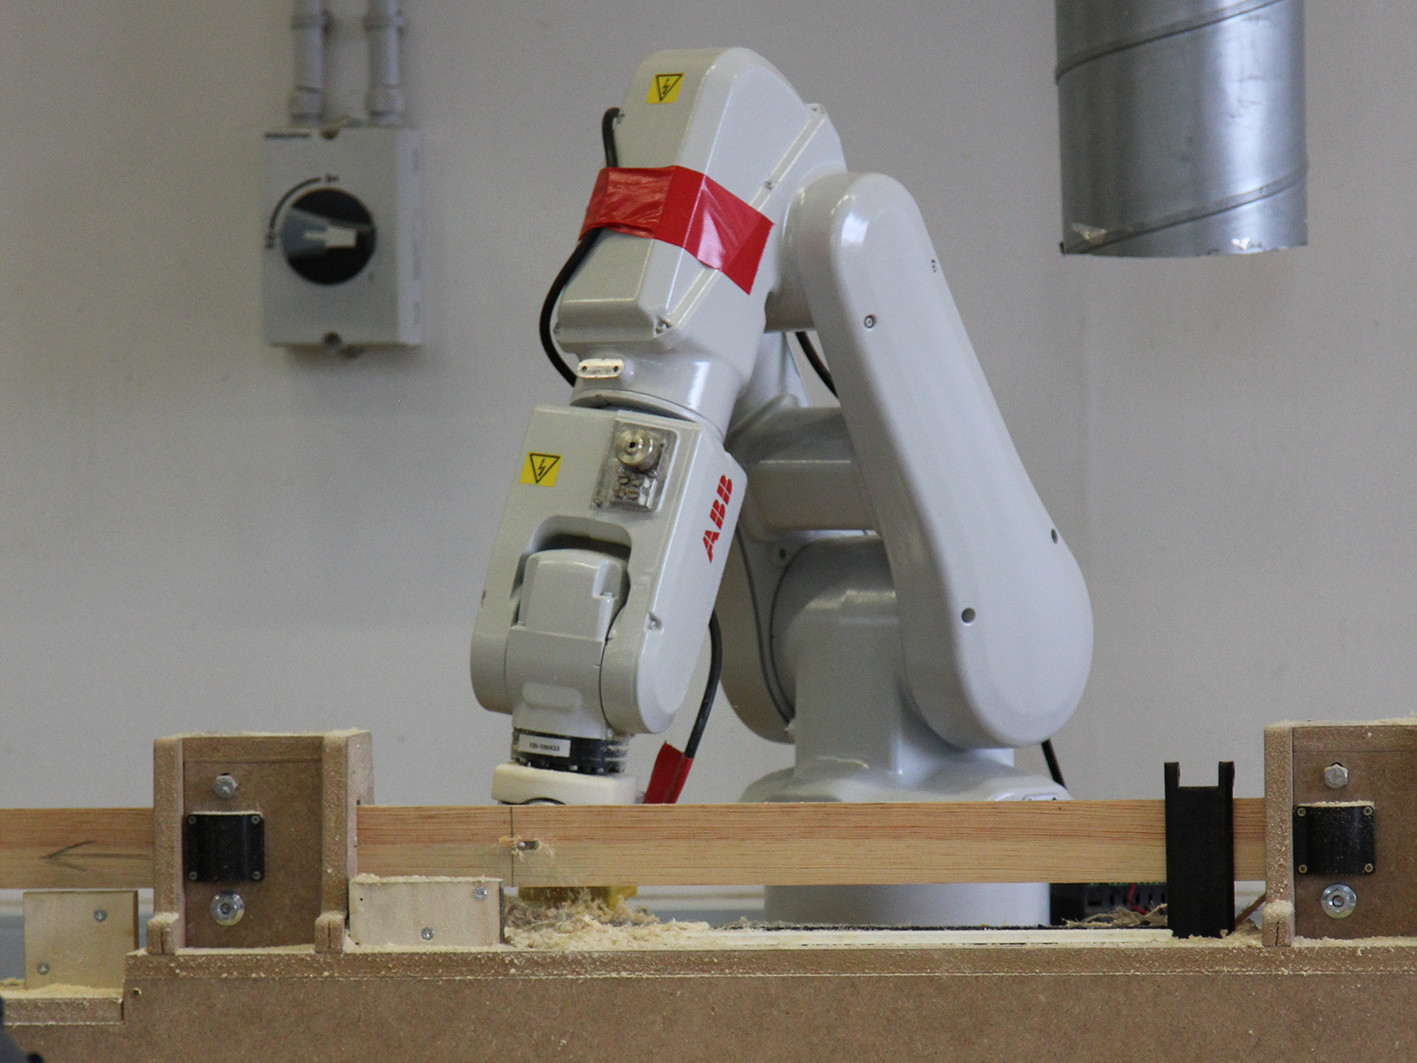
\includegraphics[width=0.48\textwidth]{clc.jpg}\label{fig:clc}}
		\hspace*{\fill}
		\subfloat[][Timber lattice]{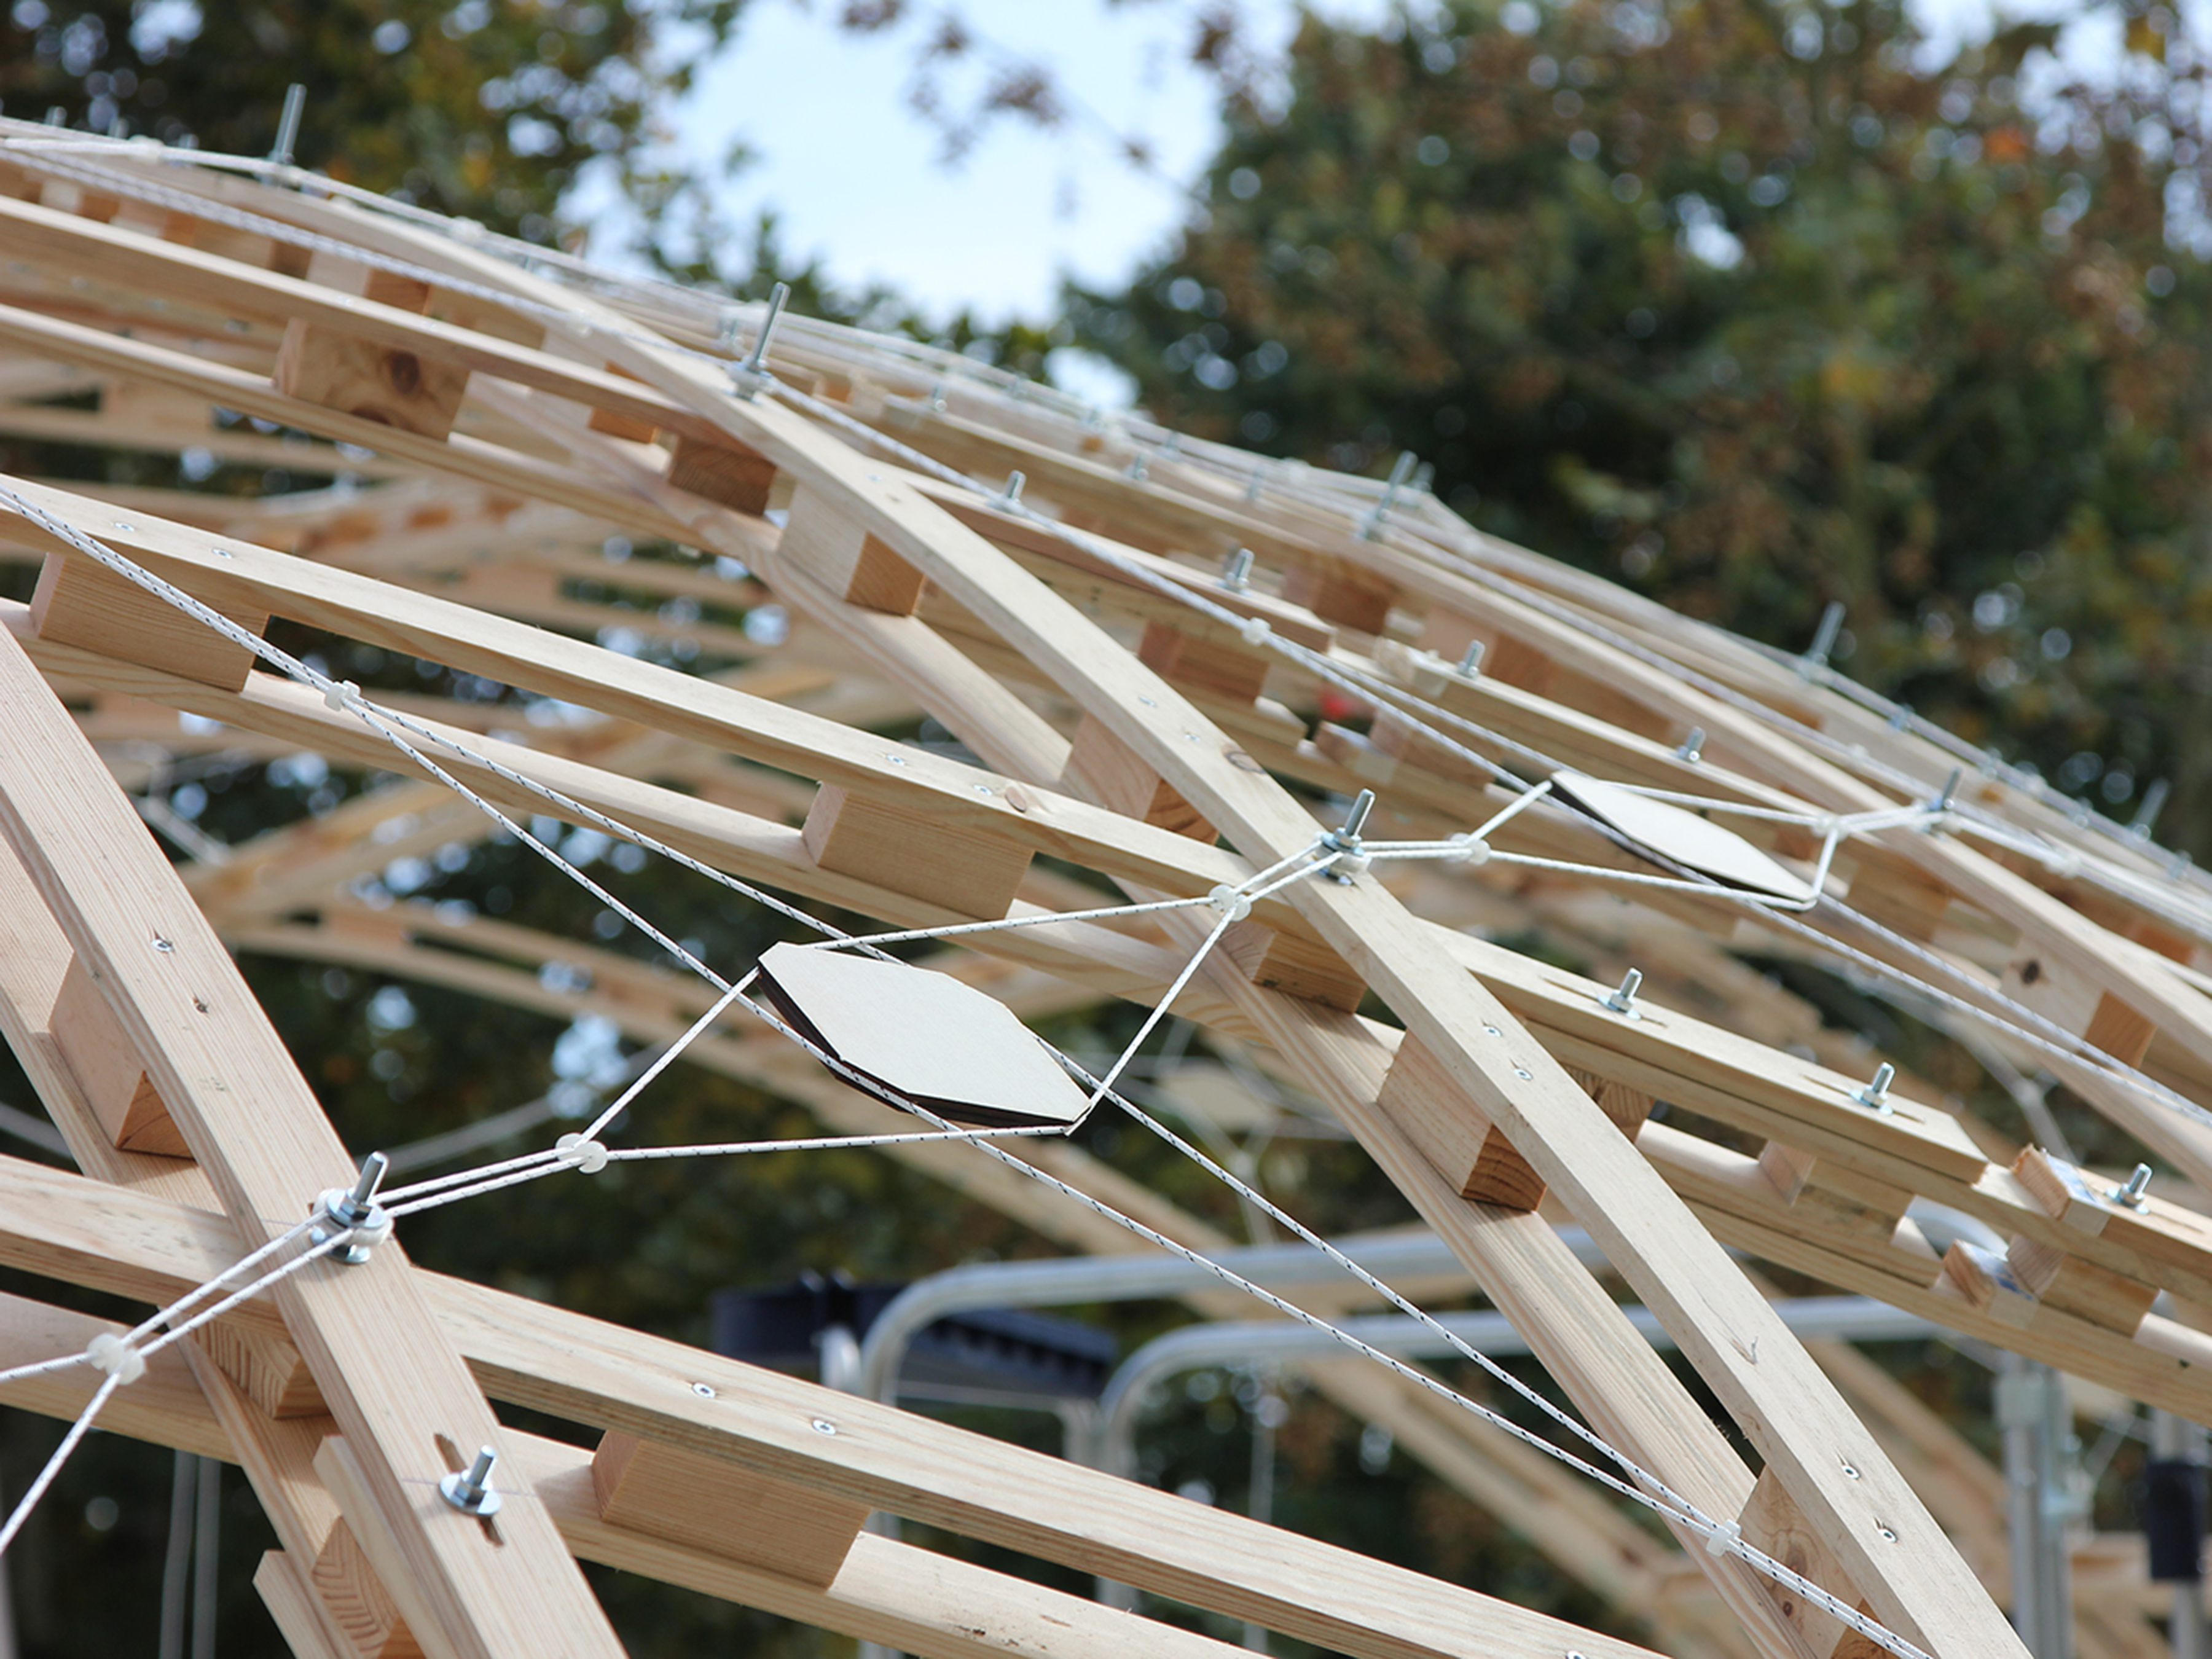
\includegraphics[width=0.48\textwidth]{clc2.jpg}\label{fig:clc2}}
		\vspace{10pt}
		\captionof{figure}[Timber gridshell built in 2016 in Champs-sur-Marne, France]{Timber gridshell built in 2016 in Champs-sur-Marne, France.}
		\label{fig:clc2016}
		%
		\vspace{0.5cm}
		%
		\subfloat[][Interior view]{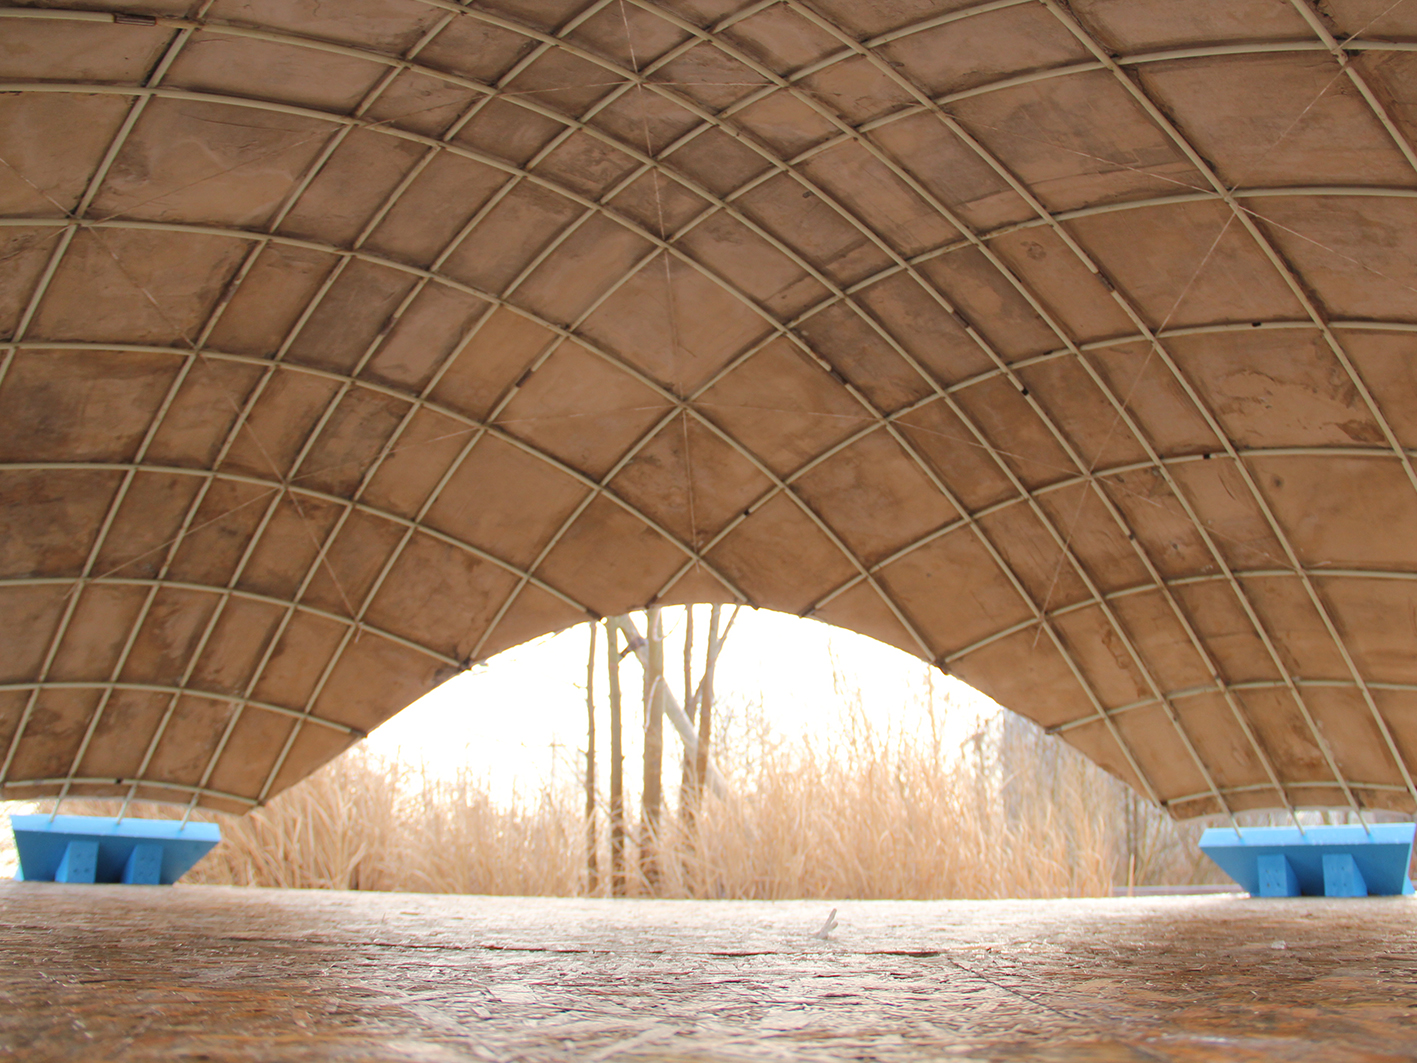
\includegraphics[width=0.48\textwidth]{booby2.jpg}\label{fig:booby1}}
		\hspace*{\fill}
		\subfloat[][Exterior view]{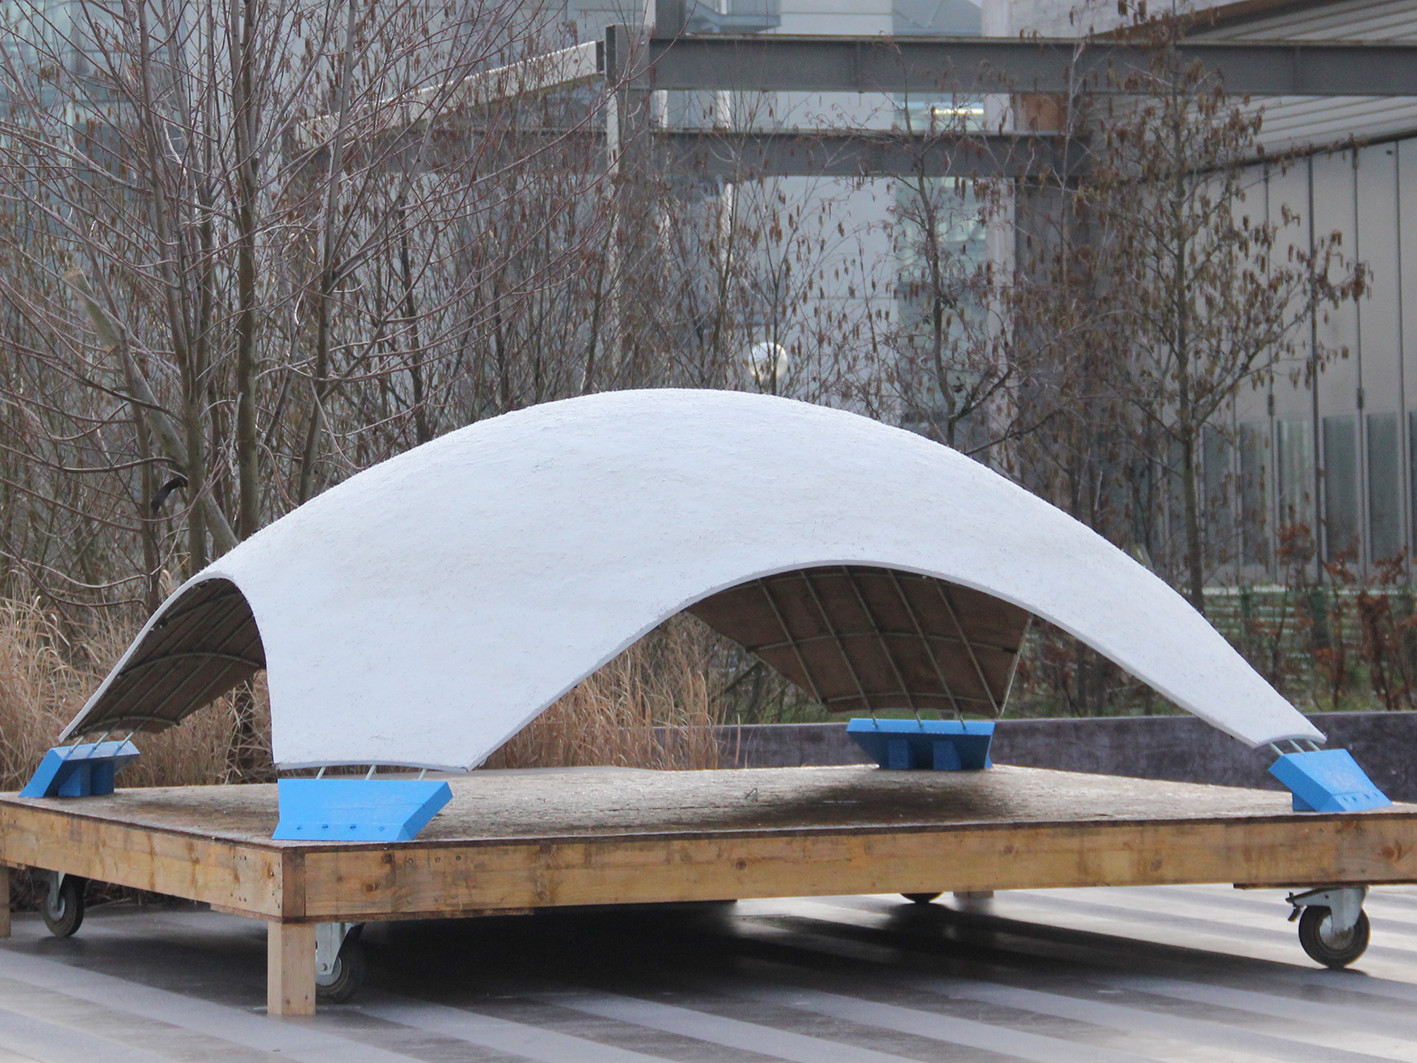
\includegraphics[width=0.48\textwidth]{booby.jpg}\label{fig:booby2}}
		\vspace{10pt}
		\captionof{figure}[Hybrid structural skin built in 2016 in Champs-sur-Marne, France]{Hybrid structural skin built in 2016 in Champs-sur-Marne, France.}
		\label{fig:booby}
	\end{fullpage}
\end{figure}

\clearpage
\section{Research works on elastic gridshells : a review}\label{sec=review_research}
In this section we depict the research works that are related to elastic gridshells. Several topics have been identified to organise the review.

\subsection{Mechanics}

\subsubsection{Form-finding}

\citef{Adriaenssens2000} propose a 6-DOF discrete beam element that integrates in a dynamic relaxation solver. This element is meant for the numerical analysis of bent elements in cable net and gridshell structures.

\citef{Adriaenssens1999} present a 3-DOF discrete beam element for the form-finding of elastic rods. This element is valid only for rods that are straight in their rest configuration and that have an isotropic cross-section. \citef{Barnes1999} integrates this element for numerical analysis based on dynamic relaxation. \citef{Adriaenssens2001} observe a better stability of this element compare to their previous 6-DOF element.

\citef{Barnes2013} try to take account for torsional behaviour in slender rods with anisotropic cross-section. They do not resort to any additional degree of freedom. Instead, they monitor the (geometric) torsion of a discrete space curve by computing the rotation rate between two consecutive osculating planes. This is valid only in rare specific cases where geometric torsion and mechanical torsion agree and is of little practical use.

\citef{DAmico2014} and later \citef{Poulsen2015} implement the 6-DOF beam element developed earlier by \citef{Adriaenssens2000} and use it for the form-finding of gridshells.

\citef{DuPeloux2015} and \citef{Lefevre2017} propose a new 4-DOF element that takes account for both bending and torsion behaviours of slender rods. It relies on the Bishop frame and the notion of parallel transport. It is based on a circular spline interpolation. This element is valid for rods with anisotropic cross-section as well as for rod that are not straight in their rest configuration. They also formulate an elastic joint for the modeling of grids of interconnected beams.

\citef{DAmico2016} propose a similar approach but use a Catmull-Rom spline interpolation. However, dealing with boundary conditions is harder with this interpolation as it requires an additional node.

\citef{Vaulot2016} revisit the benefits of using scale physical models for the form-finding of elastic gridshells. The grids are made out of Nitinol, a super-elastic material, to make sure the models will always work in the elastic domain of the material.

\citef{Bessini2017} propose a beam element based on the Reissner-Simo geometrically exact beam model. Their formulation is compatible with the dynamic relaxation method.

\subsubsection{Stability}

\citef{Bulenda2001} investigate for dome and barrel vault gridshells how imperfections can influence buckling.

\citef{Mesnil2015a} explore the influence of permanent bending pre-stress on the buckling capacity of strained gridshells. They show that for reasonably sized single-layer elastic gridshells the bending pre-stress does not influence the shape of the buckling modes. They give a simplified formula to estimate the buckling capacity of elastic gridshells under funicular loading.

\citef{Mesnil2015a} compare the linear buckling of non braced quadrangular gridshells and kagome gridshells.

\citet{Lefevre2015} explore the buckling of triangulated single-layer elastic gridshells with a dome-like shape. In their analysis they take into account the eccentricity that exists between layers and the anisotropy of the grid. They propose a simplified formula to evaluate the buckling load of such gridshells.

\subsubsection{Form-structure interaction}

\citef{Malek2012} study how corrugation in shapes affect the mechanics of gridshells.

\citef{Jensen2013} propose to interconnect several gridshells to form a stronger structure. \citef{Filz2015} also investigate the properties of interconnected gridshells but for the purpose of kinematic effects.

\subsubsection{Robustness}

\citet{Tayeb2013} study how the high level of redundancy in a gridshell enhance its resistance to collapse. They show that because of the redundancy, a pseudo ductile behaviour of the structure is still observable when a brittle material is used (such as GFRP).

\subsubsection{Implementation}

\citef{Douthe2007}, \citef{Toussaint2007}, \citef{Olsson2012}, \citef{Poulsen2015} discuss the implementation details of the dedicated form-finding algorithm they have built.

\subsection{Geometry}

\subsubsection{Generation of Chebychev nets}

In \citetitle{IL10}, \citef[]{IL10} study the uniform mesh net with square cells. They propose a classification for suspended nets (pp.~68-69) and give an inventory of common problems such as overlapping and singularities. They explain how to build valuable physical models for hanging nets (pp.~50-55) and how to measure them with either close-range stereo-photogrammetry, a simple measuring table or the parallel light measurement technique (pp.~130-134). Finally, they propose a geometric method to find Chebyshev meshes from a given curved shape called the \emph{compass method} (pp.~140-141).

\citef{Bouhaya2009} propose an alternative to the compass method for finding gridshell meshes on an imposed surface. This method consists in numerically dropping a grid onto a fixed shape. The simulation is achieved with a dynamic explicit finite element solver. Therefore, the proposed method can take into account the real mechanics of the grid, which is not possible with the compass method.

\citef{Bouhaya2014} implement the compass method in a geometry software. For a fixed mesh pitch and starting point they parametrically generate a large number of discrete guidelines on the surface. The generation of a guideline is controlled by a vector of angles controlling the expansion on the surface. The method is then coupled with a genetic algorithm to find meshes where the curvature of the elements is minimised.

\citef{Lafuente2012} propose a variational approach to find grids that minimize the curvature of the elements. This is done by introducing penalty energies. Consequently, the mesh is allowed to move away from the imposed shape and the bars are allowed to dilate from their initial length.

\citef{DuPeloux2011} implement the compass method in \grasshopper{}. They use it to design two large-scale gridshells in composite material in 2011 \cite{Baverel2012} and 2013 \Cite{DuPeloux2016}.

\citef{Lefevre2015} propose an extended compass method that take into account the eccentricity between the layers of rods. This gap is generally due to the connection system.

\citef{Masson2017} prove the existence of a global smooth Chebyshev net on complete, simply connected surfaces when the total absolute curvature is bounded by $2\pi$. In his thesis, \citef{Masson2017b} study the conditions of existence of Chebyshev nets with singularities and give methods to construct them.

\citef{Pone2016} propose a tool similar to the ones developed by \citef{DuPeloux2011} and \citef{Bouhaya2014}.

\subsubsection{Morphogenesis}

\citef{Douthe2016} propose a reverse approach. Instead of trying to fit a mesh on an imposed surface, they construct discrete surfaces that embed the required properties. They show that the dual mesh of an isoradial mesh is a Chebyshev net. They give a method to construct such nets.

\citef{Mesnil2017} propose various methods to generate construction-aware discrete surfaces. Some of them are applicable to gridshells, for instance to produce twist-free grids of grids with planar quadrangular panels.

\subsection{Material}

\citef{Douthe2010a} look for new materials that could surpass wood when building elastic gridshells. They use Ashby's selection method to show that composite materials in glass fibre reinforced polymers are good candidates. \citef{Douthe2006} build the first structure of this kind.

\citef{Kotelnikova2013} extend the previous approach to draw some recommendations for the selection of materials for actively-bent structures.

\citef{Kotelnikova2012} studies the long term behaviour of pultruded GFRP rods subject to permanent combined bending and torsion stresses.

\subsection{Technology}

\subsubsection{Erection}
In \citetitle{IL10}, \citef{IL10} propose various methods for erecting elastic gridshells.
\citef{Quinn2014} review several gridshell projects and their erection methods. They question the potential of air-inflated membrane cushions for the erection of strained gridshells. \citef{Quinn2016} investigate the benefits of pneumatic falsework to erect strained gridshells.

\citef{Liuti2016} present an inflatable membrane technology for the erection of post-formed timber gridshells. They test it on a small-scale structure.

\subsubsection{Cladding}
\citef{Lafuente2014} try to further improve the efficiency of deployable gridshells by using the cladding membrane to brace the structure. Although this solution is less stiff than the usual ones, it does enhance the deployability and reduce the work spent in the bracing stage.

\citef{Cuvilliers2017} develop a concept of a hybrid structural skin, that is an elastic gridshell in composite material braced by a thin fibre reinforced concrete skin. The gridshell serves as a formwork to the concrete skin and the concrete skin is pored directly on the deformed grid. The connection enable a tight collaboration between the structural grid an the concrete, so that the skin is bracing the gridshell.

\subsubsection{Optimization}
\citef{DAmico2015} describe a procedure to optimise timber gridshell cross-sections. The  optimisation is done for a given load case and relatively to the generated stresses. Nevertheless, this optimisation process does not take into account the buckling behaviour of the structure, which usually prevails in such lightweight structures.

\subsubsection{Robotisation}
Robotisation is investigated in recent timber gridshell projects such as the ZA pavilion \cite{Mork2016} and the pavilion built at the ENPC in 2016.\footnote{This pavilion has been published on the web~: \url{http://thinkshell.fr/freeform-wooden-gridshell-2016/}.} Robotic design and manufacturing of timber structures is further explored by \citef{Menges2016}.

\section{Conclusion}

In this chapter, we have tried to immerse ourselves in depth and experience in the complexity of these structures. After a brief description of the concept, we have established two thorough reviews. The first review is dedicated to built elastic gridshell projects from the 1960s to the present day. This brief history draws the potential of these structures, particularly in terms of formal expression and structural performance. Far from confining them to a particular style of architecture, it underlines their great variety and richness. The second review is dedicated to a literature review on all research fields related to this topic (geometry, structure, materials, software).

\clearpage
